\section{Adaptive Signal Processing}

\subsection{The Least Mean Square (LMS) Algorithm}

\noindent{}a. The AR(2) process defined in the coursework has the following general form:

\begin{align}
x(n) = a_1 x(n-1) + a_2 x(n-2) + \eta(n) \label{eq:ar_ref}
\end{align}

\noindent{}where $\eta(n) \sim \mathcal{N}(0,\sigma_{\eta}^2)$. Since the correlation matrix $\textbf{R}_x = \mathbb{E}\{\textbf{x}(n)\textbf{x}(n)^T\}$, where $\textbf{x}(n)=[x(n-1), x(n-2)]^T$, the entries of the matrix are:

\begin{align*}
\textbf{R}_x &= 
\begin{bmatrix}
\mathbb{E}\{x(n-1)x(n-1)\} \ \mathbb{E}\{x(n-1)x(n-2)\} \\ 
\mathbb{E}\{x(n-2)x(n-1)\} \ \mathbb{E}\{x(n-2)x(n-2)\}
\end{bmatrix}
\end{align*} 

\noindent{}In order to determine the entries, we multiply (\ref{eq:ar_ref}) with $x(n-k)$ and obtain:

\begin{align*}
x(n)x(n-l) = a_1 x(n-1)x(n-k) + a_2 x(n-2)x(n-l) + \eta(n)x(n-k)
\end{align*}

\noindent{}By taking expectations, we get:

\begin{align*}
\gamma(k) = \mathbb{E}\{x(n)x(n-k)\} =  a_1 \mathbb{E}\{x(n-1)x(n-k)\} + a_2  \mathbb{E}\{x(n-2)x(n-k)\}  + \mathbb{E}\{\eta(n)x(n-k)\}
\end{align*}

\noindent{}The above equation can be simplified and 3 simultaneous equations can be generated to obtain the entries of the correlation matrix:

\begin{align*}
\gamma(0) &= a_1 \gamma(1) + a_2\gamma(2) + \sigma_{\eta}^2 \\
\gamma(1) &= a_1 \gamma(0) + a_2\gamma(1) \\
\gamma(2) &= a_1 \gamma(1) + a_2\gamma(0)
\end{align*}

\noindent{}Solving the simultaneous equations with $a_1=0.1$, $a_2=0.8$ and $\sigma_{\eta}^2=0.25$, we obtain the ACF matrix:

\begin{align*}
\textbf{R}_x &= 
\begin{bmatrix}
\mathbb{E}\{x(n-1)x(n-1)\} \ \mathbb{E}\{x(n-1)x(n-2)\} \\ 
\mathbb{E}\{x(n-2)x(n-1)\} \ \mathbb{E}\{x(n-2)x(n-2)\}
\end{bmatrix}
=
\begin{bmatrix}
\gamma(0) \ \gamma(1) \\ 
\gamma(1) \ \gamma(0)
\end{bmatrix}
= 
\begin{bmatrix}
\frac{25}{27} \ \frac{25}{54} \\ 
\frac{25}{54} \ \frac{25}{27}
\end{bmatrix}
\end{align*} 

\noindent{}To find the range of values for $\mu$ that will allow LMS algorithm to converge in mean, the eigenvalues of $\textbf{R}_x$ have to be found and the inequality in (\ref{eq:convergence}) has to be satisfied.

\begin{align}
0 \ < \ \mu \ < \ \frac{2}{\lambda_{max}} \label{eq:convergence}
\end{align}

\noindent{}If the inequality is satisfied, the LMS algorithm will converge to the Winer-Hopf solution. The maximum eigenvalue of $\textbf{R}_x$ is 1.3889 and thus as long as $0 \ < \ \mu \ < \ 1.44$, the LMS algorithm will converge.

\begin{figure}[H]
\centering{}
\includegraphics[width=0.32\textwidth]{part3/ar_lms_mu_1_realisation}
\includegraphics[width=0.32\textwidth]{part3/ar_lms_mu_100_realisation}
\caption{Analysis of Effects of Different Step Size on Convergence Speed of LMS Alogirthm}
\end{figure}

\noindent{}b. The LMS adaptive predictor using $N=1000$ samples of $x(n)$ was implemented. Results of 1 realization and the average of 100 realizations are shown in the figure above for $\mu=0.01$ and $\mu=0.05$. Analyzing the squared prediction error curves, it is clear that on average we obtain faster convergence when $\mu=0.05$. This is exactly as expected because larger values of $\mu$ enable a steeper decent of the error surface.

\begin{figure}[H]
\centering{}
\includegraphics[width=0.32\textwidth]{part3/time_average_mu_01}
\includegraphics[width=0.32\textwidth]{part3/time_average_mu_05}
\caption{Time-Average of Steady State Error for $\mu=0.01$ and $\mu=0.05$}
\end{figure}

\noindent{}c. The figure above shows the steady-state of the ensemble-average learning curves using 100 independent trials of the experiment. Based on the 100 independent realizations, the excess mean square error (EMSE), misadjustment and theoretical misadjustment are calculated and the results are shown in the table below. The empirical misadjustment are slightly higher than the theoretical values. Regardless, it is abundantly clear that having a smaller step size introduces a much smaller EMSE and results in a smaller misadjustment value. However, as observed above, having a smaller step size causes the rate of convergence to be slow.  

\begin{table}[H]
\centering
\begin{tabular}{|c|c|c|c|c|}
\hline
mu   & EMSE   & Empirical Misadjustment 	& Theoretical Misadjustment		\\ \hline
0.01 & 0.0032 & 0.0128                 	& 0.0093                   		\\ \hline
0.05 & 0.124  & 0.0496                 	& 0.0463                  		\\ \hline
\end{tabular}
\end{table}

\noindent{}d. The graphs below show how the coefficients evolve over time. For the rest of the section, most graphs will show the evolution of coefficients, averaged over 100 realizations, and thus it is good to get a feel of what the graphs look like for just 1 realization. Real world adaptive filters will often work with only 1 realization of a random signal. Looking more specifically at the evolution of coefficients for $\mu=0.05$ for 1 realization, it is clear that speed has been traded off for steady-state error. The amount of variation around the ideal values is significant.

\begin{figure}[H]
\centering{}
\includegraphics[width=0.32\textwidth]{part3/ar_coefficients_evolution_mu_01_1_trial}
\includegraphics[width=0.32\textwidth]{part3/ar_coefficients_evolution_mu_05_1_trial} \\ 
\includegraphics[width=0.32\textwidth]{part3/ar_coefficients_evolution_mu_01}
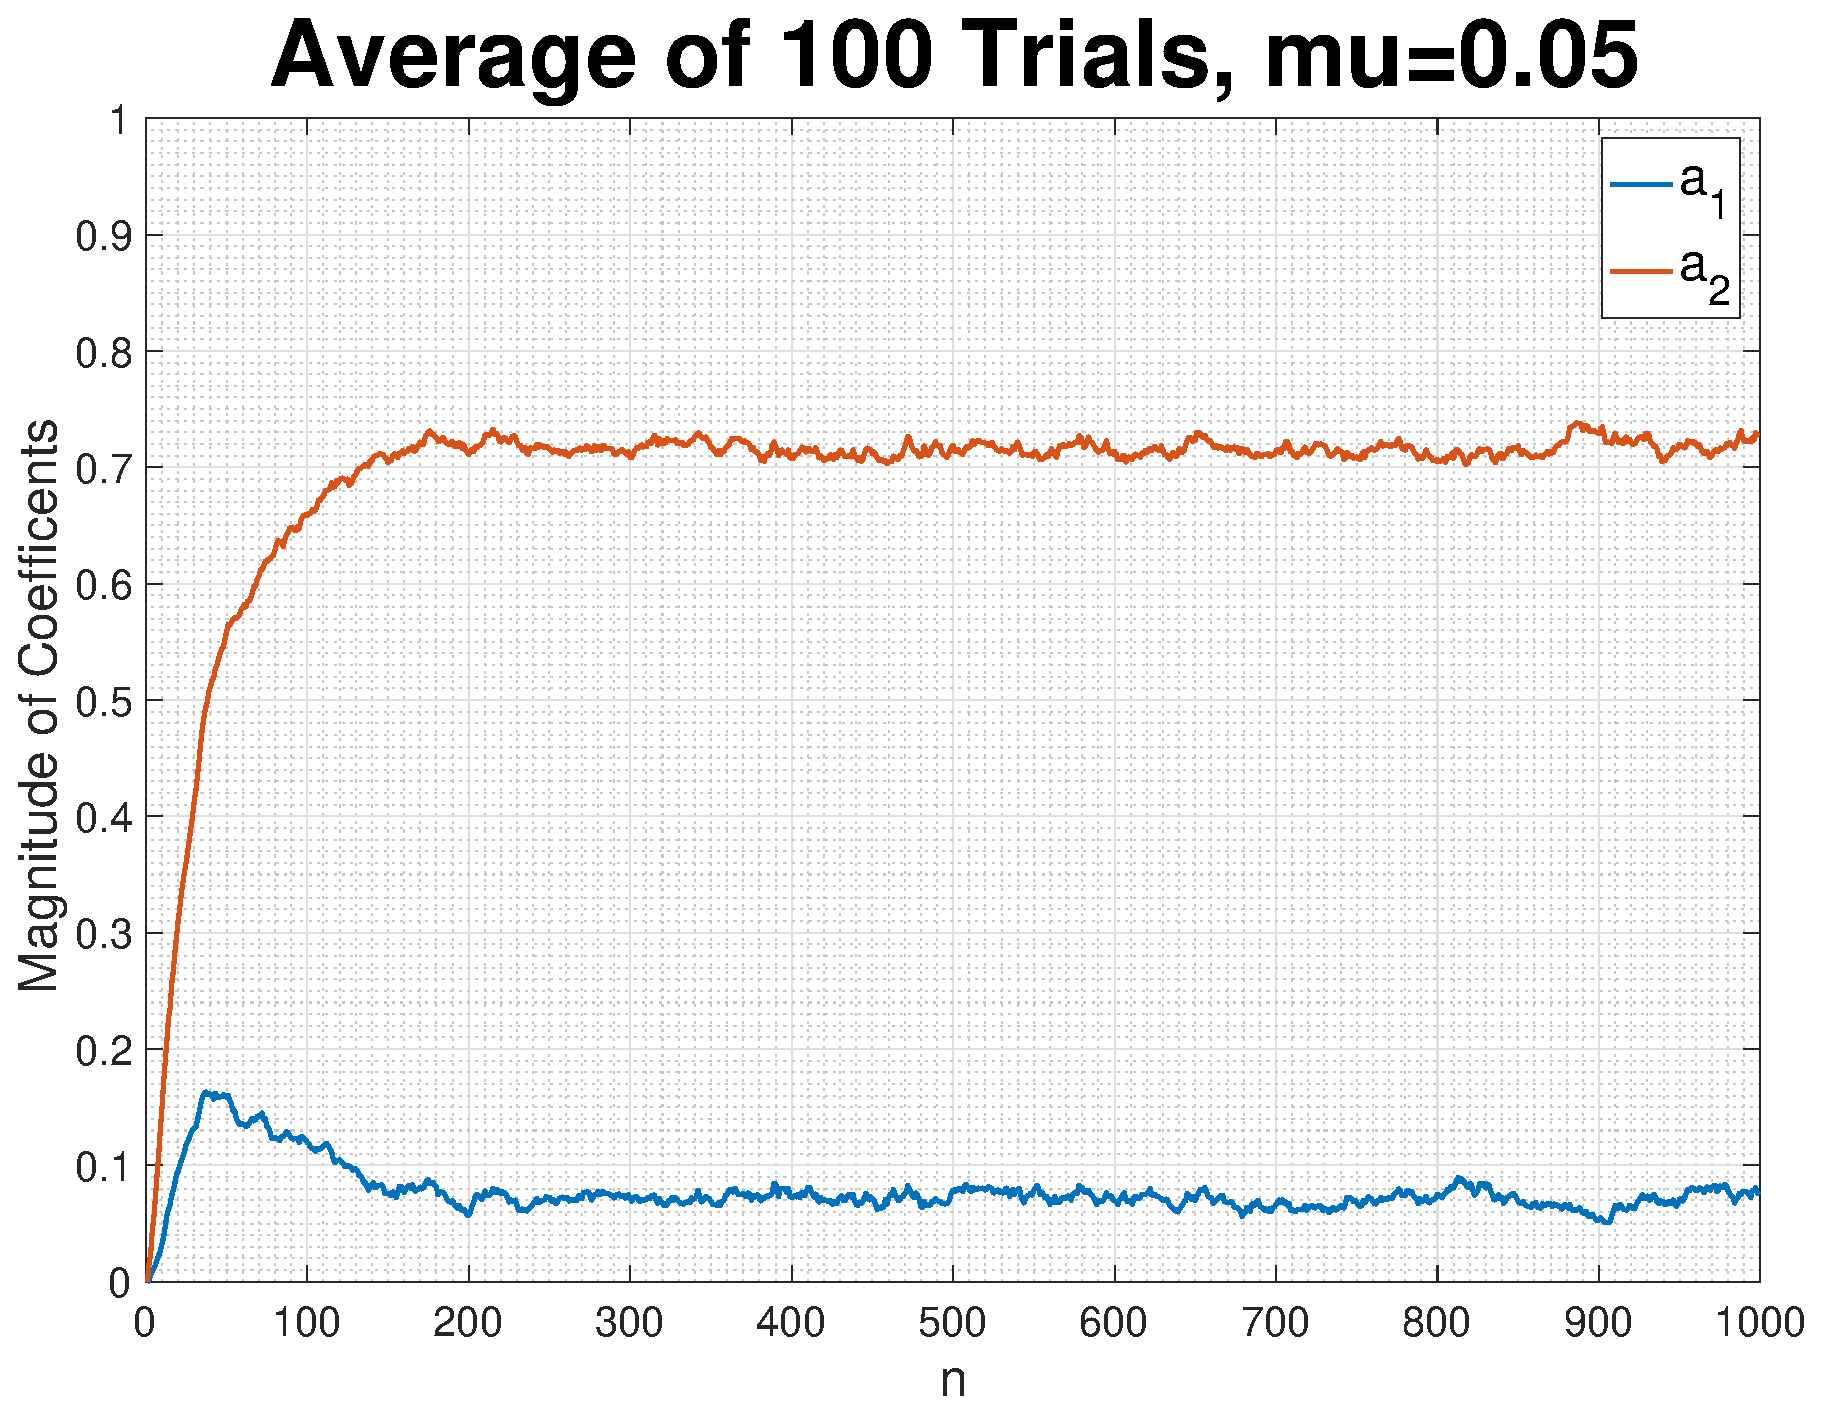
\includegraphics[width=0.32\textwidth]{part3/ar_coefficients_evolution_mu_05}
\caption{Evolution of Coefficients for 1 Trial and 100 Trial, for $\mu=0.01$ and $\mu=0.05$}
\label{fig:steady_state_convergence}
\end{figure}

\noindent{}Next, to answer the question directly, we observe Figure \ref{fig:steady_state_AR}. It is clear that for both coefficients, having a small value of $\mu$ results in the steady state value that is much closer to the ideal values of $a_1=0.1$ and $a_2=0.8$. In addition, having a small value of $\mu$ results in a much smaller steady-state variance. However, looking at Figure \ref{fig:steady_state_convergence}, we find that setting $\mu=0.01$, we do not approach the steady state value until the 900th iteration. In contrast, using $\mu=0.05$, the algorithm converges in about 200 iterations.

\begin{figure}[H]
\centering{}
\includegraphics[width=0.32\textwidth]{part3/steady_state_ar_coeff_1}
\includegraphics[width=0.32\textwidth]{part3/steady_state_ar_coeff_2}
\caption{Steady State Values of Coefficients $a_1$ and $a_2$, for $\mu=0.01$ and $\mu=0.05$}
\label{fig:steady_state_AR}
\end{figure}

\noindent{}e. In order to minimize the cost function with respect to $\textbf{w}$, we differentiate it with respect to $\textbf{w}$ and set the derivative to 0. Mathematically, we obtain:

\begin{align}
J(n) &= \frac{1}{2}\Bigg(e^2(n)+\gamma||\textbf{w}(n)||^2\Bigg) \label{eq:cost_func}\\ 
\frac{\partial J}{\partial \textbf{w}} &= e(n)\frac{\partial e}{\partial \textbf{w}} + \gamma \textbf{w}(n) = 0 \nonumber
\end{align}

\noindent{}We can express the error as $e(n)=\textbf{x}(n) - \textbf{w}^T(n)\textbf{x}(n)$. If we make the substitution and differentiate we get,

\begin{align*}
\frac{\partial e}{\partial \textbf{w}} = \frac{\partial}{\partial \textbf{w}}\Bigg(\textbf{x}(n) - \textbf{w}^T(n)\textbf{x}(n)\Bigg) = -\textbf{x}(n)
\end{align*}

\noindent{}Then,

\begin{align*}
\frac{\partial J}{\partial \textbf{w}} = -\gamma \textbf{w}(n) + e(n)
\end{align*}

\noindent{}Now, using the gradient decent method to reach the optimal value of $w$, we have to implement the update equation presented in (\ref{eq:w_update}).

\begin{align}
\textbf{w}(n) = \textbf{w}(n) - \mu \nabla_{w}J(n) \label{eq:w_update}
\end{align}

\noindent{}Substituting the derivative of the cost function into (\ref{eq:w_update}), we obtain:

\begin{align}
\textbf{w}(n+1) &= \textbf{w}(n) - \mu \Bigg(-\gamma \textbf{w}(n) + e(n)\Bigg)\textbf{x}(n) \nonumber\\
\textbf{w}(n+1) &= (1-\mu\gamma)\textbf{w}(n) - \mu e(n)\textbf{x}(n) \label{eq:leaky_lms}
\end{align}

\noindent{}Therefore, we have shown that the leaky LMS equation quoted in the coursework and derived in (\ref{eq:leaky_lms}) is equivalent to minimizing the cost function shown in (\ref{eq:cost_func}).\\

\noindent{}f. The graphs shown in Figure \ref{fig:leaky_lms} show evolution of coefficients for different values of $\mu$ and $\gamma$ using the leaky LMS algorithm. The steady-state values do not converge to the true values of $a_1$ and $a_2$. In fact, the larger the value of $\gamma$, the greater the steady-state bias. The Weiner-Hopf solution was briefly mentioned above. It gives the optimal weights calculated using the autocorrelation matrix, $\textbf{R}$, and the cross correlation vector, $\textbf{p}$:

\begin{align*}
\textbf{w}_{opt} = \textbf{R}^{-1}\textbf{p}
\end{align*}

\noindent{}The LMS algorithm, under certain bounds on the value of $\mu$, iteratively arrives at the Weiner-Hopf solution. The motivation of the algorithm is to prevent inverting the autocorrelation matrix. The leaky LMS however does not converge to the Wiener-Hopf solution. The leaky LMS minimizes a cost function that is slightly different to the cost function that the LMS algorithm minimizes and thus it converges to:

\begin{align*}
\lim_{k \rightarrow \infty} \mathbb{E}[\textbf{w}_{k}] = (\textbf{R} + \gamma\textbf{I})^{-1}\textbf{p}
\end{align*}

\noindent{}The additional, $\gamma\textbf{I}$ term causes a bias that means that the leaky LMS does not actually converge to the Wiener-Hopf solution. In fact, using the autocorrelation matrix $\textbf{R}_x$ derived above and  $\textbf{p} = [\gamma(1), \gamma(2)]^T$, we can mathematically determine the values to which the Leaky-LMS algorithm converges:

\begin{table}[H]
\centering
\begin{tabular}{|c|c|c|}
\hline
$\gamma$ & $a_1$     & $a_2$     \\ \hline
0.1   & 0.1542 & 0.3919 \\ \hline
0.5   & 0.1626 & 0.4992 \\ \hline
0.9   & 0.1319 & 0.7076 \\ \hline
\end{tabular}
\end{table}

\noindent{}Notice that the graphs confirm the theoretical results. Different values of $\gamma$ lead to the Leaky-LMS algorithm settling to different values. The leaky LMS displays the same properties, discussed above, with respect to $\mu$.

\begin{figure}[H]
\centering{}
\includegraphics[width=0.32\textwidth]{part3/leaky_mu_01_gamma_01}
\includegraphics[width=0.32\textwidth]{part3/leaky_mu_01_gamma_05}
\includegraphics[width=0.32\textwidth]{part3/leaky_mu_01_gamma_09}
\includegraphics[width=0.32\textwidth]{part3/leaky_mu_05_gamma_01}
\includegraphics[width=0.32\textwidth]{part3/leaky_mu_05_gamma_05}
\includegraphics[width=0.32\textwidth]{part3/leaky_mu_05_gamma_09}
\caption{Effect of increasing $\gamma$ on the Steady State Values of Coefficients $a_1$ and $a_2$, for $\mu=0.01$ and $\mu=0.05$}
\label{fig:leaky_lms}
\end{figure}

\subsection{Adaptive Step Sizes}

\noindent{}a. Using the LMS algorithm, we have shown the effect that $\mu$ has on the convergence time as well as the misadjustment. Depending on the application, we can select a $\mu$ to satisfy constraints on convergence time or overshoot or steady-state error. The non-varying nature of $\mu$ makes the LMS algorithm computationally cheap. However, keeping a constant $\mu$ has certain shortcomings. A major shortcoming is that certain choices $\mu$ can cause the algorithm to diverge instead of converging to a solution. \\

\noindent{}The Gradient Adaptive Step Size (GASS) algorithms allow $\mu$ to be time-varying. The algorithms are generally implemented such that the steady-state learning rates approach 0, thereby ensuring stability and convergence. The adaptive nature of the step sizes gives us the flexibilty to vary $\mu$ according to the error that is incurred. The three GASS algorithms specified in the coursework all modify the step size according to the following equation:

\begin{align*}
\mu(n+1)=\mu(n) + \rho e(n) \textbf{x}^T(n)\bm{\psi}(n)
\end{align*}

\noindent{}In all algorithms the value of $\rho$ is a constant while $\bm{\psi}$ is time-varying. The value of $\bm{\psi}$ is altered using the following equations:

\begin{align*}
\text{Benveniste}&: \bm{\psi}(n)=[\textbf{I}-\mu(n-1)\textbf{x}(n-1)\textbf{x}^T(n-1)]\bm{\psi}(n-1) + e(n-1)\bm{x}(n-1) \\
\text{Ang \& Farhang}&: \bm{\psi}(n)=\alpha\bm{\psi}(n-1) + e(n-1)\bm{x}(n-1), \ \ \ \ \ 0 < \alpha < 1 \\
\text{Matthew \& Xie}&: \bm{\psi}(n)=e(n-1)\bm{x}(n-1)
\end{align*}

\noindent{}Notice that in the Benveniste algorithm, the update equation for $\bm{\psi}$ is an adaptive low-pass filter with the instantaneous gradient $e(n-1)x(n-1)$ as the input. This algorithm has the ability to deal with noise in the gradient estimate. The Ang \& Farhang algorithm modifies the Benveniste algorithm by turning the update equation for $\bm{\psi}$ from an adaptive to a non-adaptive low-pass filter. The algorithm trades computational complexity for slightly worse convergence properties. The Matthew \& Xie algorithm goes a step further and removes the low-pass filtering that the other two algorithms perform on the instantaneous gradient. This makes the algorithm even faster, however once again convergence properties are sacrificed for speed.\\

\noindent{}The graphs below show the weight error curves for just 1 trial of the algorithms. It is clear that all of the GASS algorithms perform significantly better than the LMS algorithm which do not vary the value of $\mu$.

\begin{figure}[H]
\centering{}
\includegraphics[width=0.32\textwidth]{part3/convergence_of_weights}
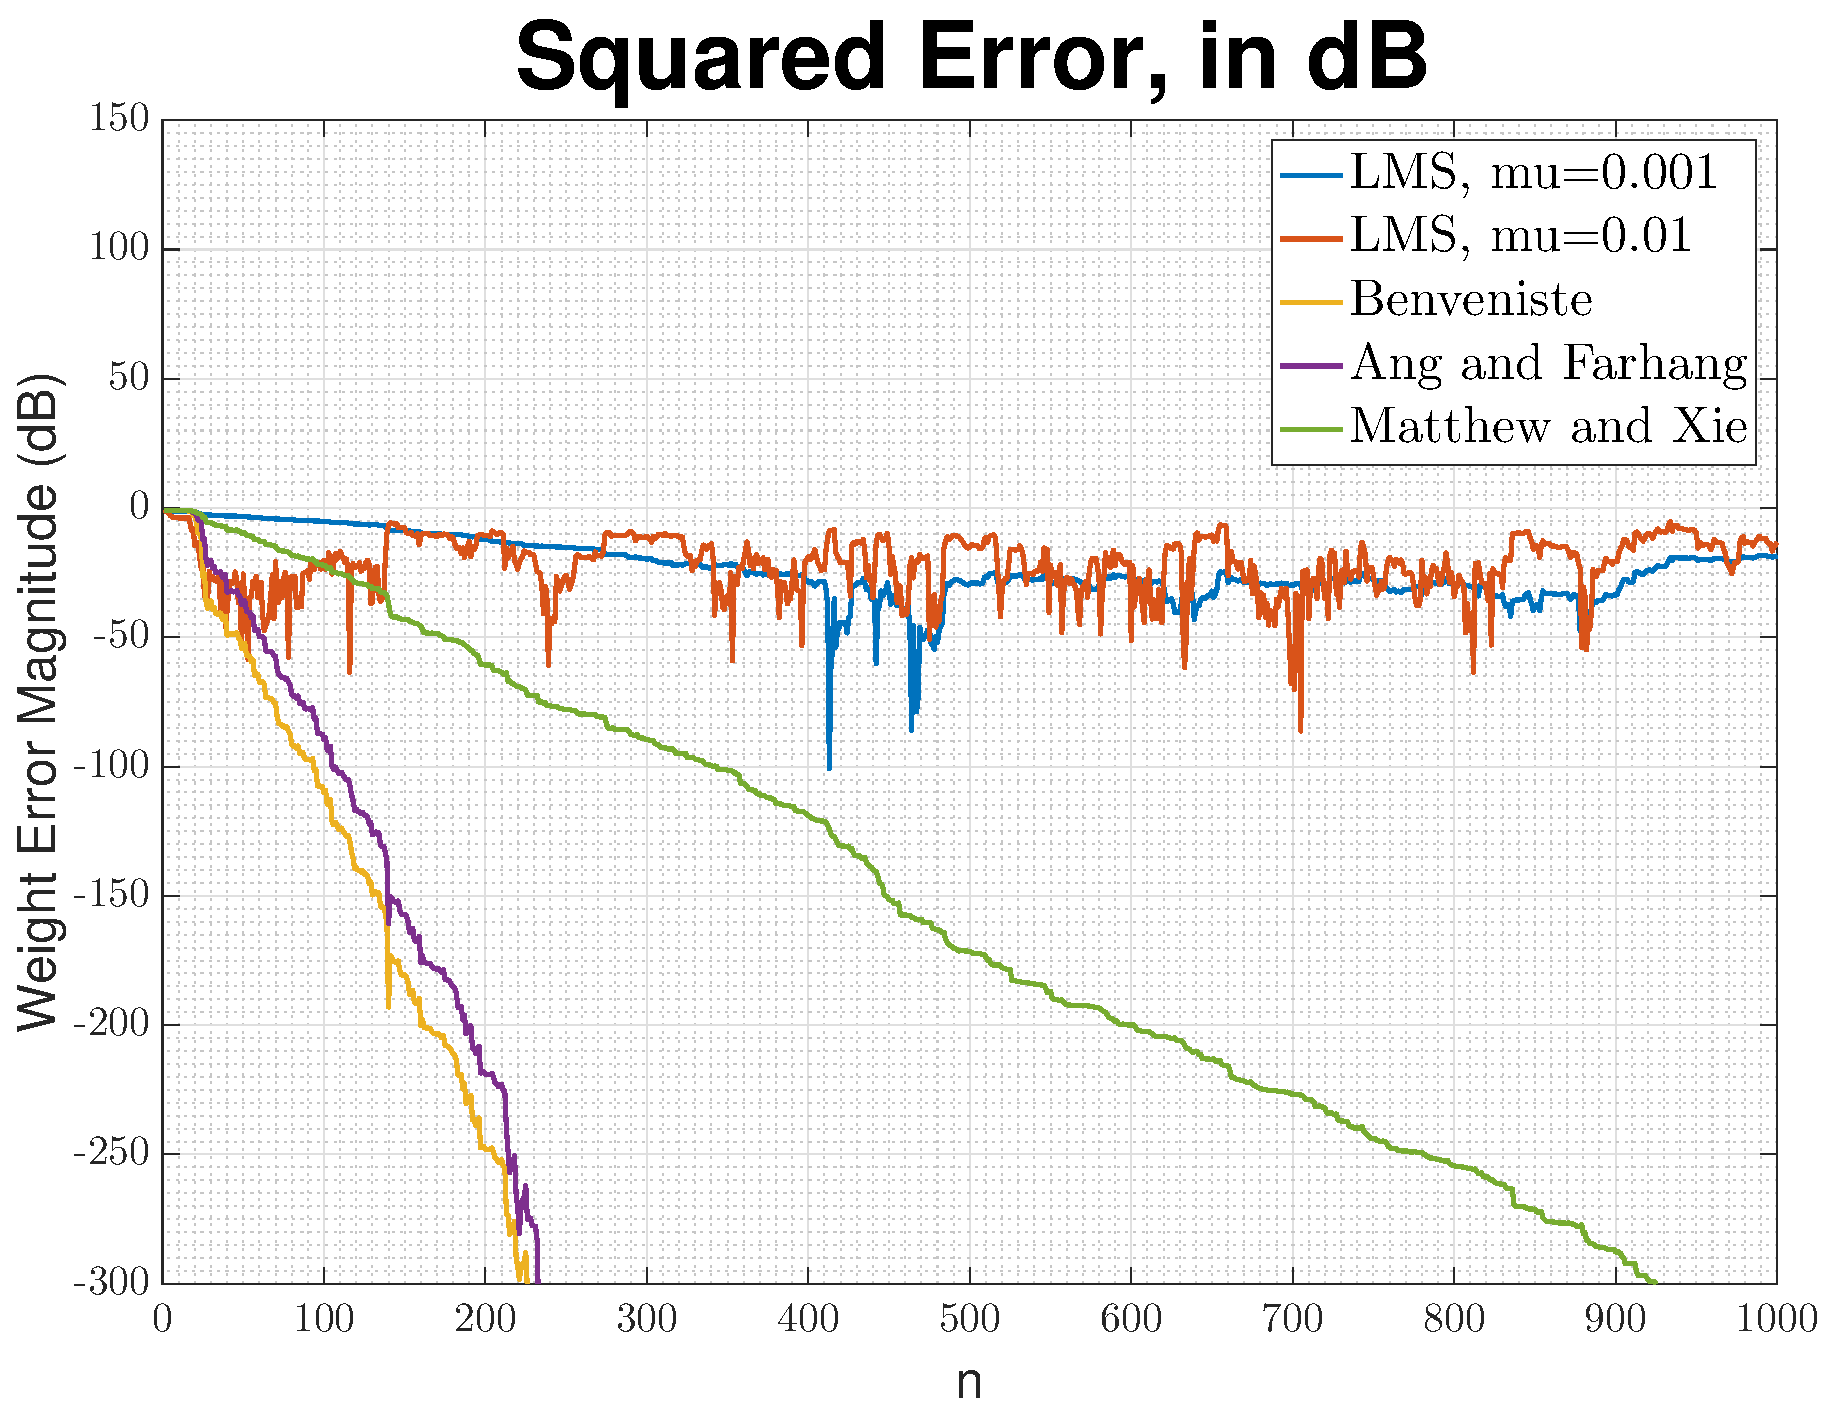
\includegraphics[width=0.32\textwidth]{part3/convergence_of_weights_db}
\caption{Comparison of Convergence Time using Adaptive Step Sizes and Standard LMS Algorithms}
\end{figure}

\noindent{}The averaged results of a 100 trials are graphed below. The first thing to notice is that the LMS alogrithms with constant $\mu$ do not converge to the correct weights. The results obtained for the GASS algorithms are exactly as expected. The Benveniste algorithm, which is computationally the most expensive, is able to converge the fastest. The next to follow is the Ang \& Farhang algorithm. Notice that although the Mattew \& Xie algorithm performs the worst amongst the GASS algorithms, it is still significantly better than the LMS algorithms without adaptive step-sizes. Notice also that all GASS algorithms do not have offsets and converge to the true weights.


\begin{figure}[H]
\centering{}
\includegraphics[width=0.32\textwidth]{part3/convergence_of_weights_averaged}
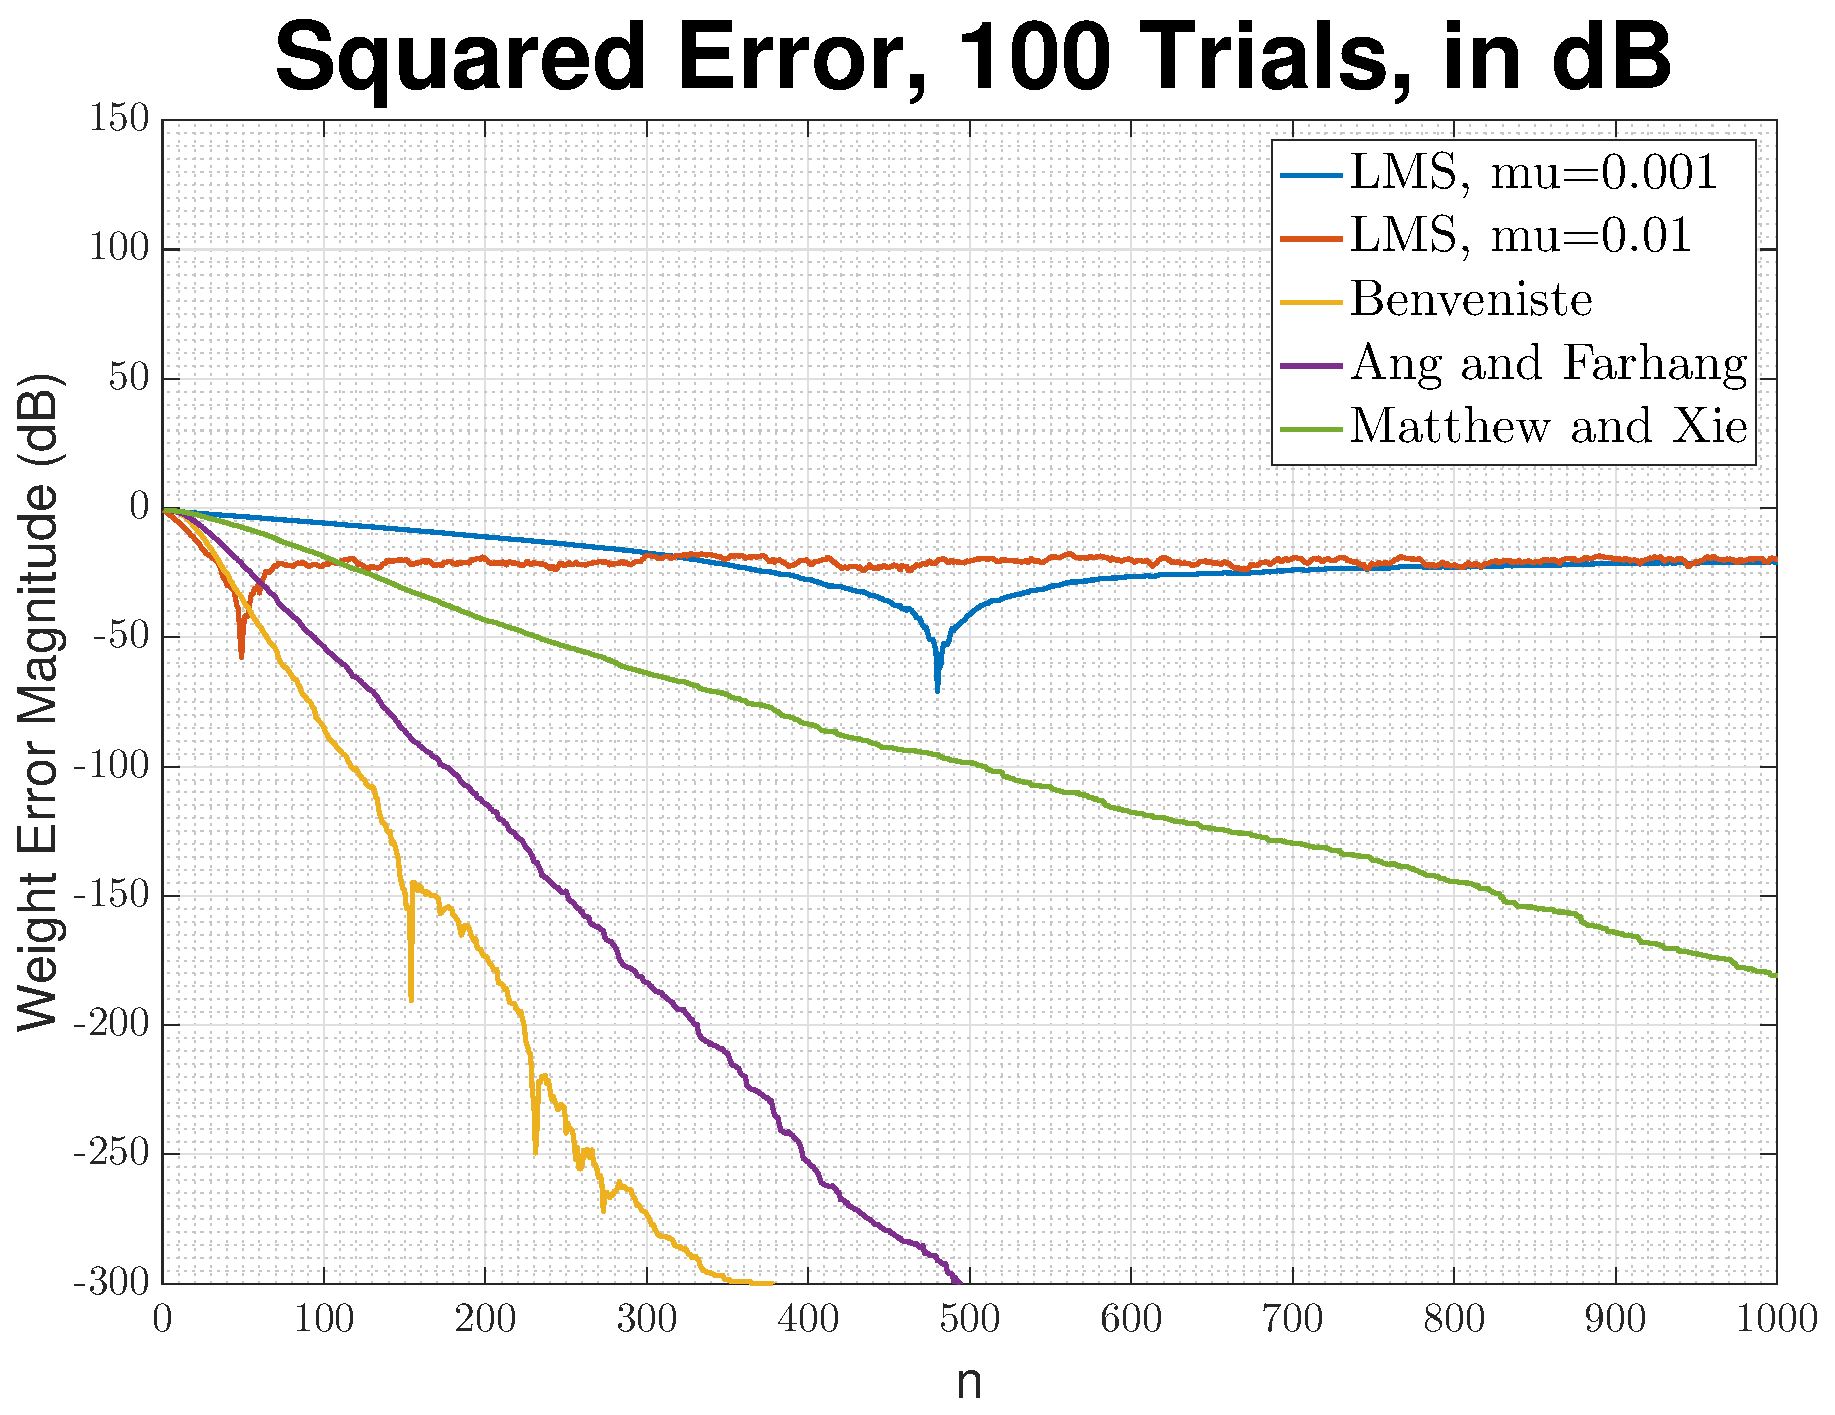
\includegraphics[width=0.32\textwidth]{part3/convergence_of_weights_averaged_db}
\caption{Studying Convergence Time by Averaging Weights over 100 Random Realisations}
\end{figure}


\noindent{}b. The normalised LMS (NLMS) algorithm has the following update equation:

\begin{align}
\textbf{w}(n+1) = \textbf{w}(n) + \frac{\beta}{\epsilon + ||\textbf{x}||^2} e(n)\textbf{x}(n)\label{eq:nlms_algo}
\end{align}

\noindent{}To show that the update equation in (\ref{eq:nlms_update}) based upon the \textit{a posteriori} error $e_p(n)=d(n)-\textbf{x}^T(n)\textbf{w}(n+1)$ is equivalent to the NLMS algorithm, we first multiply both sides by $\textbf{x}^T(n)$. 

\begin{align}
\textbf{w}(n+1) &= \textbf{w}(n) + \mu e_p(n)\textbf{x}(n) \label{eq:nlms_update}\\
\textbf{x}^T(n)\textbf{w}(n+1) &= \textbf{x}^T(n)\textbf{w}(n) + \textbf{x}^T(n) \mu e_p(n) \textbf{x}(n) \nonumber
\end{align}

\noindent{}Next, we add $\textbf{d}(n)$ to both sides and rearrange:

\begin{align}
\textbf{d}(n)+\textbf{x}^T(n)\textbf{w}(n+1) &= \textbf{d}(n)+\textbf{x}^T(n)\textbf{w}(n) + \textbf{x}^T(n) \mu e_p(n) \textbf{x}(n) \nonumber\\
\textbf{d}(n)-\textbf{x}^T(n)\textbf{w}(n) &= \textbf{d}(n)-\textbf{x}^T(n)\textbf{w}(n+1) + \textbf{x}^T(n) \mu e_p(n) \textbf{x}(n)\label{eq:nlms_mid_proof}
\end{align}

\noindent{}Next we substitute the \textit{a posteriori} error, $e_p(n)$, and the error, $e(n)$, into (\ref{eq:nlms_mid_proof}):

\begin{align}
e(n) &= e_p(n) + \textbf{x}^T(n) \mu e_p(n) x(n) \nonumber\\
e(n) &= e_p(n) \bigg(1+\mu ||\textbf{x}||^2\bigg) \nonumber\\
e_p(n) &= \frac{e(n)}{1+\mu||\textbf{x}||^2} \label{eq:a_posteriori_error}
\end{align}

\noindent{}We can now substitute (\ref{eq:a_posteriori_error}) into the original update equation (\ref{eq:nlms_update}) and obtain the NLMS algorithm defined in (\ref{eq:nlms_algo}):

\begin{align}
\textbf{w}(n+1) &= \textbf{w}(n) + \mu \frac{e(n)}{1+\mu ||\textbf{\textbf{x}}||^2}\textbf{x}(n) \nonumber\\
&= \textbf{w}(n) + \frac{1}{\frac{1}{\mu}+ ||\textbf{\textbf{x}}||^2}e(n)\textbf{x}(n) 
\end{align}

\noindent{}Thereby proving that the update equation in (\ref{eq:nlms_update}) based the \textit{a posteriori} error with $\epsilon=\frac{1}{\mu}$ and $\beta=1$ is equivalent to the NLMS algorithm defined in (\ref{eq:nlms_algo}). Since $\epsilon$ is inversely proportional to the step size $\mu$, the algorithm does not become unstable even if $||\textbf{x}||^2$ is extremely small.

\begin{figure}[H]
\centering{}
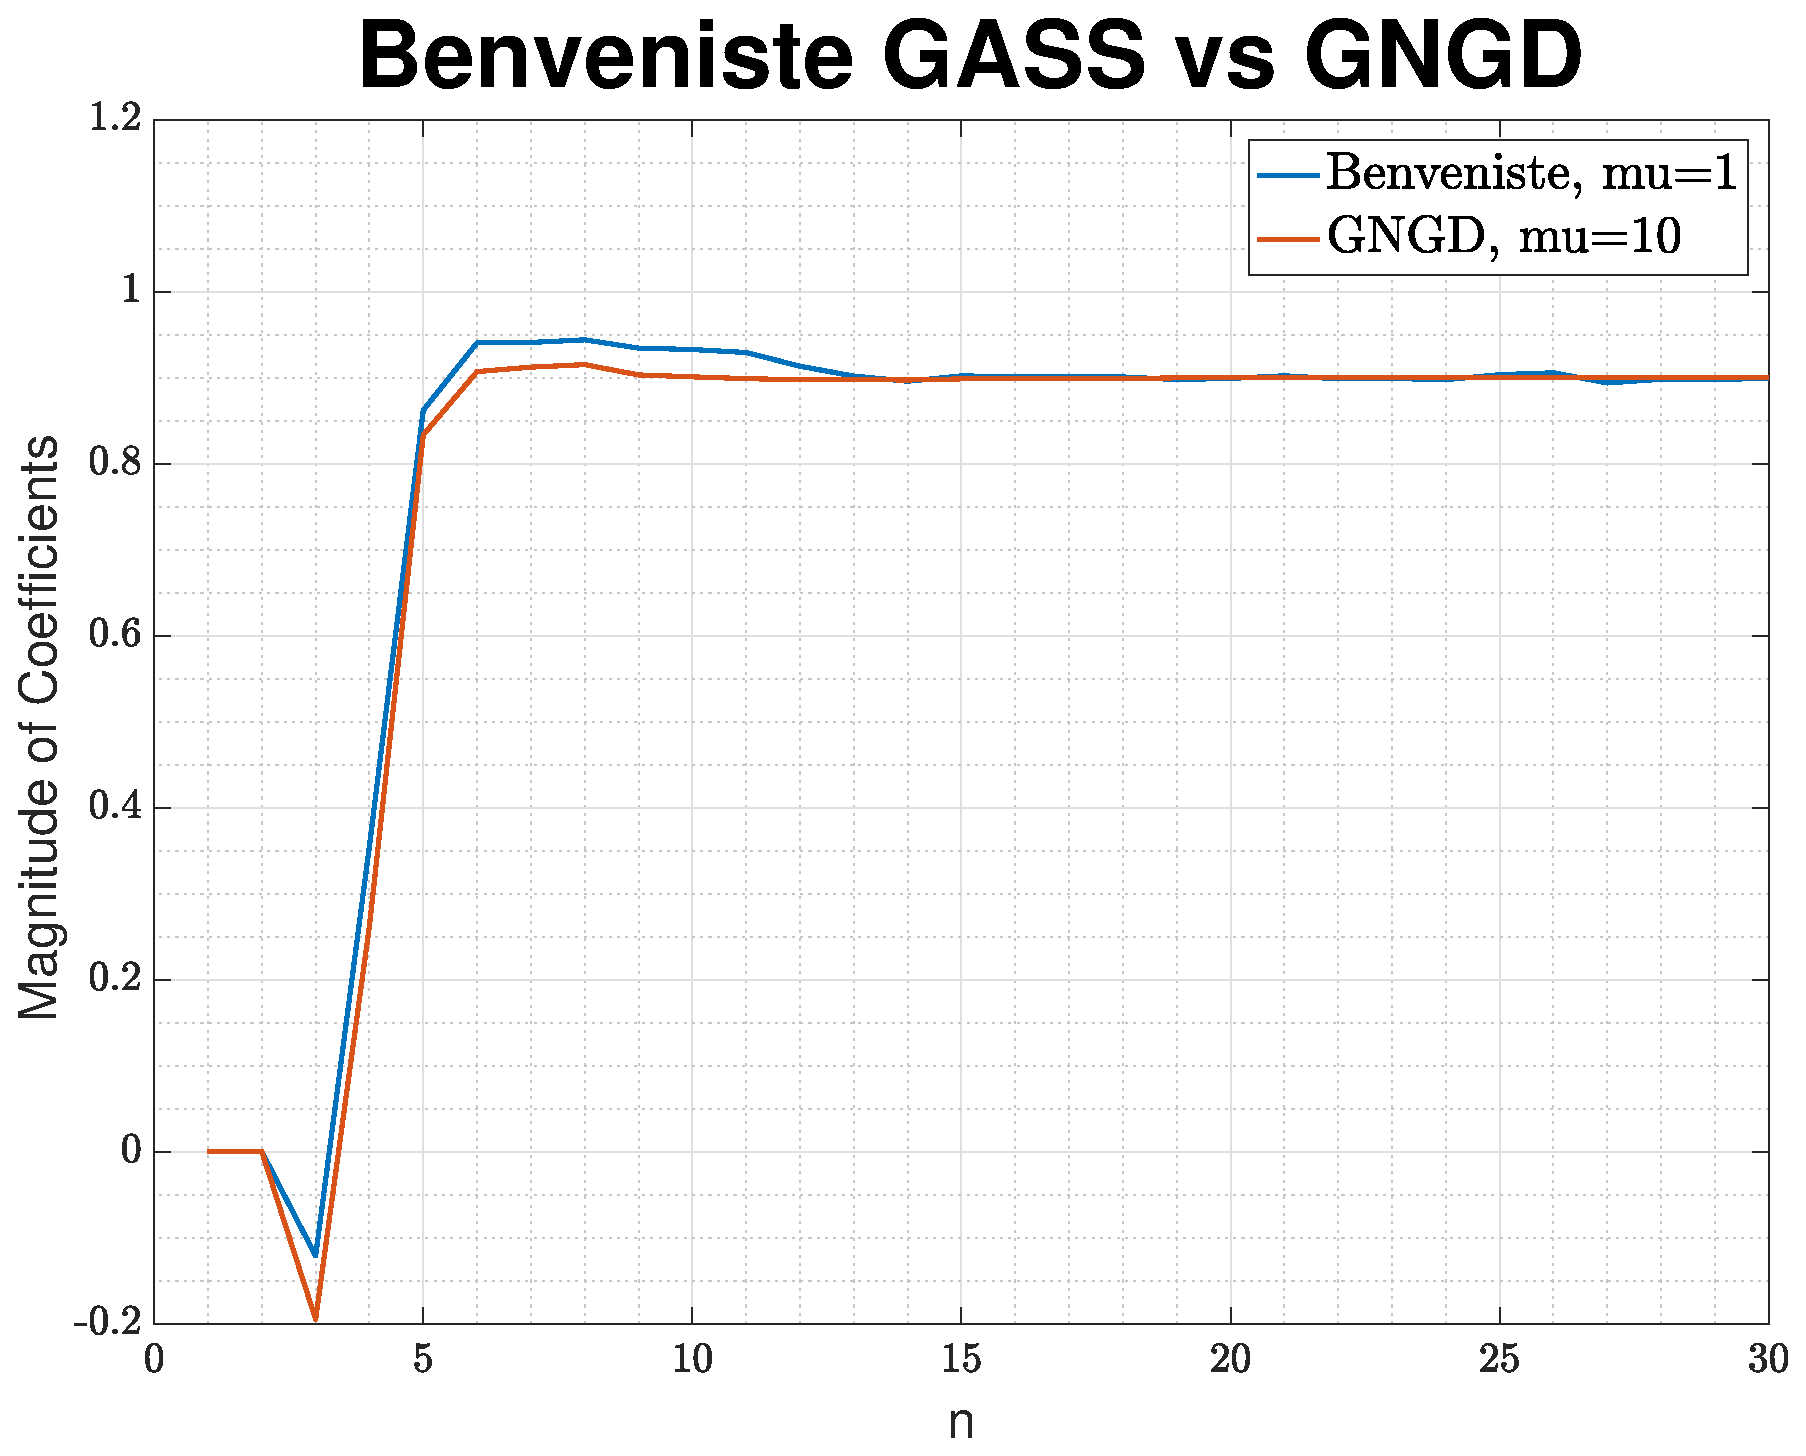
\includegraphics[width=0.32\textwidth]{part3/compare_benveniste_gngd}
\caption{Comparing Convergence Speed of GNGD and Benveniste's GASS Algorithms}
\end{figure}

\noindent{}c. From the figure above, it is clear that the Generalized Normalized Gradient Descent (GNGD) algorithm converges much faster than the Benveniste algorithm. Both algorithms are similar in the fact that they modify the learning rate in an adaptive manner. The difference lies in the fact that the GNGD algorithm modifies the learning rate in a non-linear manner. The non-linear updates provide compensation for the assumptions made in the derivation of the NLMS. The non-linear updates make the algorithm more robust and the increased stability make it effective at processing non-linear and non-stationary signals (REFERENCE MANDIC PAPER).\\

\noindent{}In terms of the computational complexity of both algorithms, the GNGD algorithm also beats the Benveniste algorithm. The number of additions and multiplications for the Benveniste algorithm are presented in the Table \ref{tab:ben}. The variable $M$ represents the model order. It is clear that the Benveniste algorithm scales quadratically with the model order. The computational complexity of the algorithm can be attributed to the outter product $\textbf{x}(n-1)\textbf{x}^T(n-1)$ that has to performed to update the value of $\bm{\psi}(n)$. 

\begin{table}[H]
\tabulinesep=0.9mm
\centering
\begin{tabu}{|c|c|c|c|}
\hline
Step                   			& Sub-Step & Multiplications & Additions \\ \hline
\multirow{6}{*}{$\bm{\psi}(n)$} 	& $\textbf{x}(n-1)\textbf{x}^T(n-1)$ 													&$M^2$         		&0\\ \cline{2-4} 
                       			& $\mu(n-1)\textbf{x}(n-1)\textbf{x}^T(n-1)$       										&$M^2$       		&0\\ \cline{2-4} 
                       			& $I-\mu(n-1)\textbf{x}(n-1)\textbf{x}^T(n-1)$    										&0        			&$M$\\ \cline{2-4} 
                       			& $[I-\mu(n-1)\textbf{x}(n-1)\textbf{x}^T(n-1)]\bm{\psi}(n-1)$       						&$M^2$ 				&$M^2-M$	\\ \cline{2-4} 
                       			& $e(n-1)\textbf{x}(n-1)$       															&$M$        		&0\\ \cline{2-4} 
                       			& $[I-\mu(n-1)\textbf{x}(n-1)\textbf{x}^T(n-1)]\bm{\psi}(n-1) + e(n-1)\textbf{x}(n-1)$  	&0          			&$M$\\ \hline 
\multirow{4}{*}{$\mu(n+1)$} 		& $\textbf{x}^T(n)\bm{\psi}(n)$ 															&$M$         		&$M-1$\\ \cline{2-4}
								& $\rho e(n)$       																		&0        			&$1$\\ \cline{2-4} 
                       			& $\rho e(n) \textbf{x}^T(n)\bm{\psi}(n)$    											&$0$        			&$1$\\ \cline{2-4} 
                       			& $\mu(n)+\rho e(n) \textbf{x}^T(n)\bm{\psi}(n)$       									&$0$ 				&$1$	\\ \hline
\multirow{3}{*}{$\textbf{w}(n+1)$}& $\mu(n)e(n)$ 																			&$0$         		&$1$\\ \cline{2-4}
								& $\mu e(n)\textbf{x}(n)$       															&$M$        			&$0$\\ \cline{2-4} 
                       			& $\textbf{w}(n) + \mu e(n)\textbf{x}(n)$    											&$0$        			&$M$\\ \hline
\multicolumn{1}{l}{}                         & \multicolumn{1}{l}{}          & \multicolumn{1}{l}{}                 & \multicolumn{1}{l}{}           \\ \hline
\multicolumn{2}{|c|}{Total}    	&\multicolumn{1}{c|}{$\mathcal{O}(M^2)$} & \multicolumn{1}{c|}{$\mathcal{O}(M^2)$} \\ \hline  
\end{tabu}
\caption{Computational Complexity of the Benveniste Algorithm}
\label{tab:ben}
\end{table}

\noindent{}Table \ref{tab:gngd} shows the computational complexity of the GNGD algorithm. It is clear that the GNGD algorithm only scales linearly with the model order. 

\begin{table}[H]
\tabulinesep=0.9mm
\centering
\begin{tabu}{|c|c|c|c|}
\hline
Step                   			& Sub-Step & Multiplications & Additions \\ \hline
\multirow{7}{*}{$\epsilon(n+1)$}	& $\textbf{x}^T(n)\textbf{x}(n-1)$ 																			&$M$         		&$M-1$\\ \cline{2-4} 
                       			& $e(n)e(n-1)$       																						&$1$       			&0\\ \cline{2-4} 
                       			& $e(n)e(n-1)\textbf{x}^T(n)\textbf{x}(n-1)$    																&$1$        			&$0$\\ \cline{2-4} 
                       			& $||\textbf{x}(n-1)||^2$       																				&$M$ 				&$M-1$	\\ \cline{2-4} 
                       			& $(\epsilon(n-1)+||\textbf{x}(n-1)||^2)^2$       															&$1$        			&1\\ \cline{2-4} 
                       			& $\rho\mu\frac{e(n)e(n-1)\textbf{x}^T(n)\textbf{x}(n-1)}{(\epsilon(n-1)+||\textbf{x}(n-1)||^2)^2}$  			&$3$          		&$0$\\  \cline{2-4}                      			
                       			& $\epsilon(n)+\rho\mu\frac{e(n)e(n-1)\textbf{x}^T(n)\textbf{x}(n-1)}{(\epsilon(n-1)+||\textbf{x}(n-1)||^2)^2}$	&$0$        			&1\\ \hline 
\multirow{5}{*}{$\textbf{w}(n+1)$}& $||\textbf{x}(n)||^2$ 																					&$M$         		&$M-1$\\ \cline{2-4} 
                       			& $\frac{\beta}{\epsilon(n) + ||\textbf{x}(n)||^2}$       													&$1$       			&1\\ \cline{2-4} 
                       			& $\frac{\beta}{\epsilon(n) + ||\textbf{x}(n)||^2}e(n)$    													&$1$        			&$0$\\ \cline{2-4} 
                       			& $\frac{\beta}{\epsilon(n) + ||\textbf{x}(n)||^2}e(n)\textbf{x}(n)$       									&$M$ 				&$M-1$	\\ \cline{2-4} 
                       			& $\textbf{w}(n)+\frac{\beta}{\epsilon(n) + ||\textbf{x}(n)||^2}e(n)\textbf{x}(n)$       						&$0$        			&$M$\\ \hline
\multicolumn{1}{l}{}                         & \multicolumn{1}{l}{}          & \multicolumn{1}{l}{}                 & \multicolumn{1}{l}{}           \\ \hline
\multicolumn{2}{|c|}{Total}    	&\multicolumn{1}{c|}{$\mathcal{O}(M)$} & \multicolumn{1}{c|}{$\mathcal{O}(M)$} \\ \hline 
\end{tabu}
\caption{Computational Complexity of the GNGD Algorithm}
\label{tab:gngd}
\end{table}


\subsection{Adaptive Noise Cancellation}

\noindent{}a. By choosing an appropriate value of $\Delta$, the Adaptive Line Enhancement (ALE) configuration can be set up such that the noise, $\eta(n)$, in the signal, $s(n)$, and the predicted input, $\textbf{u}(n)$ are uncorrelated. If the noise $\eta(n)$ and the predicted input $\textbf{u}(n)$ are uncorrelated, the noise can be suppressed and a clean signal can be obtained. To find an optimal value of $\Delta$, we start with the mean-squared error:

\begin{align*}
\mathbb{E}\bigg\{\bigg(s(n)-\hat{x}(n)\bigg)^2\bigg\} &= \mathbb{E}\bigg\{\bigg(x(n)+\eta(n)-\hat{x}(n)\bigg)^2\bigg\} \\
&=\mathbb{E}\{\eta^2(n)\} + \mathbb{E}\bigg\{\bigg(x(n)-\hat{x}(n)\bigg)^2\bigg\} + 2\mathbb{E}\bigg\{\eta(n)\bigg(x(n)-\hat{x}(n)\bigg)\bigg\}
\end{align*}

\noindent{}Expanding the mean-sqaured error shows that there are three terms that contribute to the error. Ideally, we would like the mean-squared error to be exactly equal to the noise-power, however by changing the value of $\Delta$, it is only possible to manipulate $2\mathbb{E}\bigg\{\eta(n)\bigg(x(n)-\hat{x}(n)\bigg)\bigg\}$. As such, $\Delta$ should be chosen so as to minimise $2\mathbb{E}\bigg\{\eta(n)\bigg(x(n)-\hat{x}(n)\bigg)\bigg\}$. It is important to note that since $x(n)$ and $\eta(n)$ are uncorrelated, the minimization problem reduces to minimizing $\mathbb{E}\{\eta(n)\hat{x}(n)\}$. Since $\eta(n)=v(n) + 0.5v(n-2)$ we get:

\begin{align*}
\mathbb{E}\{\eta(n)\hat{x}(n)\} &= \mathbb{E}\bigg\{\bigg( v(n) + 0.5v(n-2)\bigg) \textbf{w}^T \textbf{u}(n)\bigg\} \\
&= \mathbb{E}\bigg\{\bigg( v(n) + 0.5v(n-2)\bigg) \bigg(\sum_{i=0}^{M}w_{i}s(n-\Delta-i)\bigg)\bigg\} \\
&= \mathbb{E}\bigg\{\bigg( v(n) + 0.5v(n-2)\bigg) \bigg(\sum_{i=0}^{M}w_{i}\big(x(n-\Delta-i)+\eta(n-\Delta-i)\big)\bigg)\bigg\} 
\end{align*}

\noindent{}Again using the fact that $x(n)$ and $v(n)$ are uncorrelated:

\begin{align*}
\mathbb{E}\{\eta(n)\hat{x}(n)\} &= \mathbb{E}\bigg\{\bigg( v(n) + 0.5v(n-2)\bigg) \bigg(\sum_{i=0}^{M}w_{i}\eta(n-\Delta-i)\bigg)\bigg\} \\
&= \mathbb{E}\bigg\{\bigg( v(n) + 0.5v(n-2)\bigg) \bigg(\sum_{i=0}^{M}w_{i}\big(v(n-\Delta-i)+0.5v(n-\Delta-i-2)\big)\bigg)\bigg\}
\end{align*}

\noindent{}Thus, it is clear that for a value of $\Delta$ greater than 2, the expectation would reduce to adding the expectations of white noise samples at different time indexes, which are uncorrelated. The results presented in Figure \ref{fig:ale} corroborate these finding. Note that the top row of the figure shows the averaged results from 100 realizations, whereas the bottom row shows the overlay of 100 realizations. The ideal sinewave has been superimposed for reference. All the figures conclusively prove that for $\Delta>2$ the results obtained are significantly better. This is also corroborated by the large decrease in the mean-squared error from when $\Delta$ is increased from $2$ to $3$.

\begin{figure}[H]
\centering{}
\includegraphics[width=0.24\textwidth]{part3/delay_1}
\includegraphics[width=0.24\textwidth]{part3/delay_2}
\includegraphics[width=0.24\textwidth]{part3/delay_3}
\includegraphics[width=0.24\textwidth]{part3/delay_4}
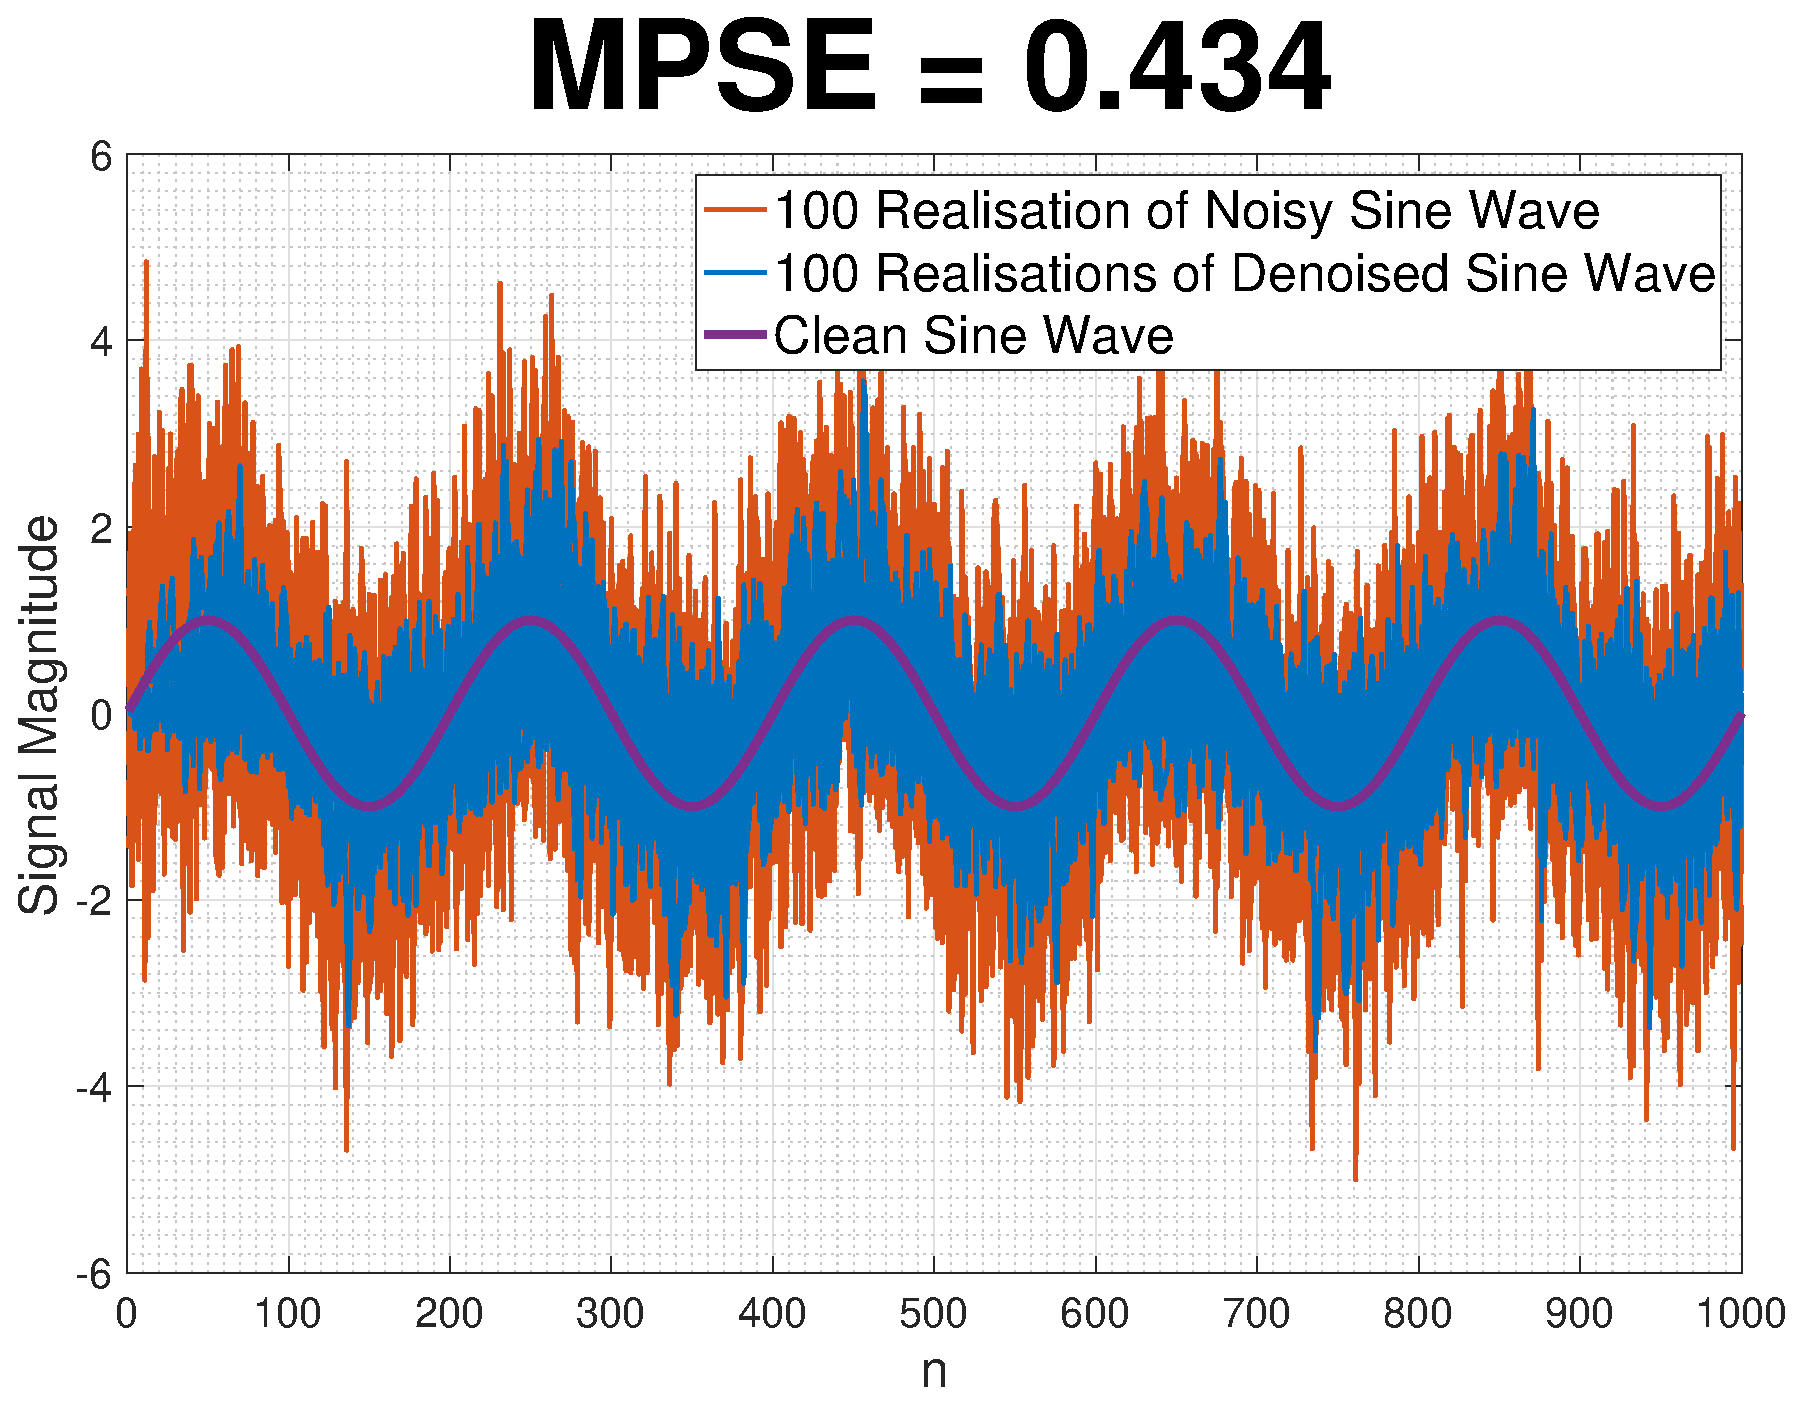
\includegraphics[width=0.24\textwidth]{part3/mpse_delay_1}
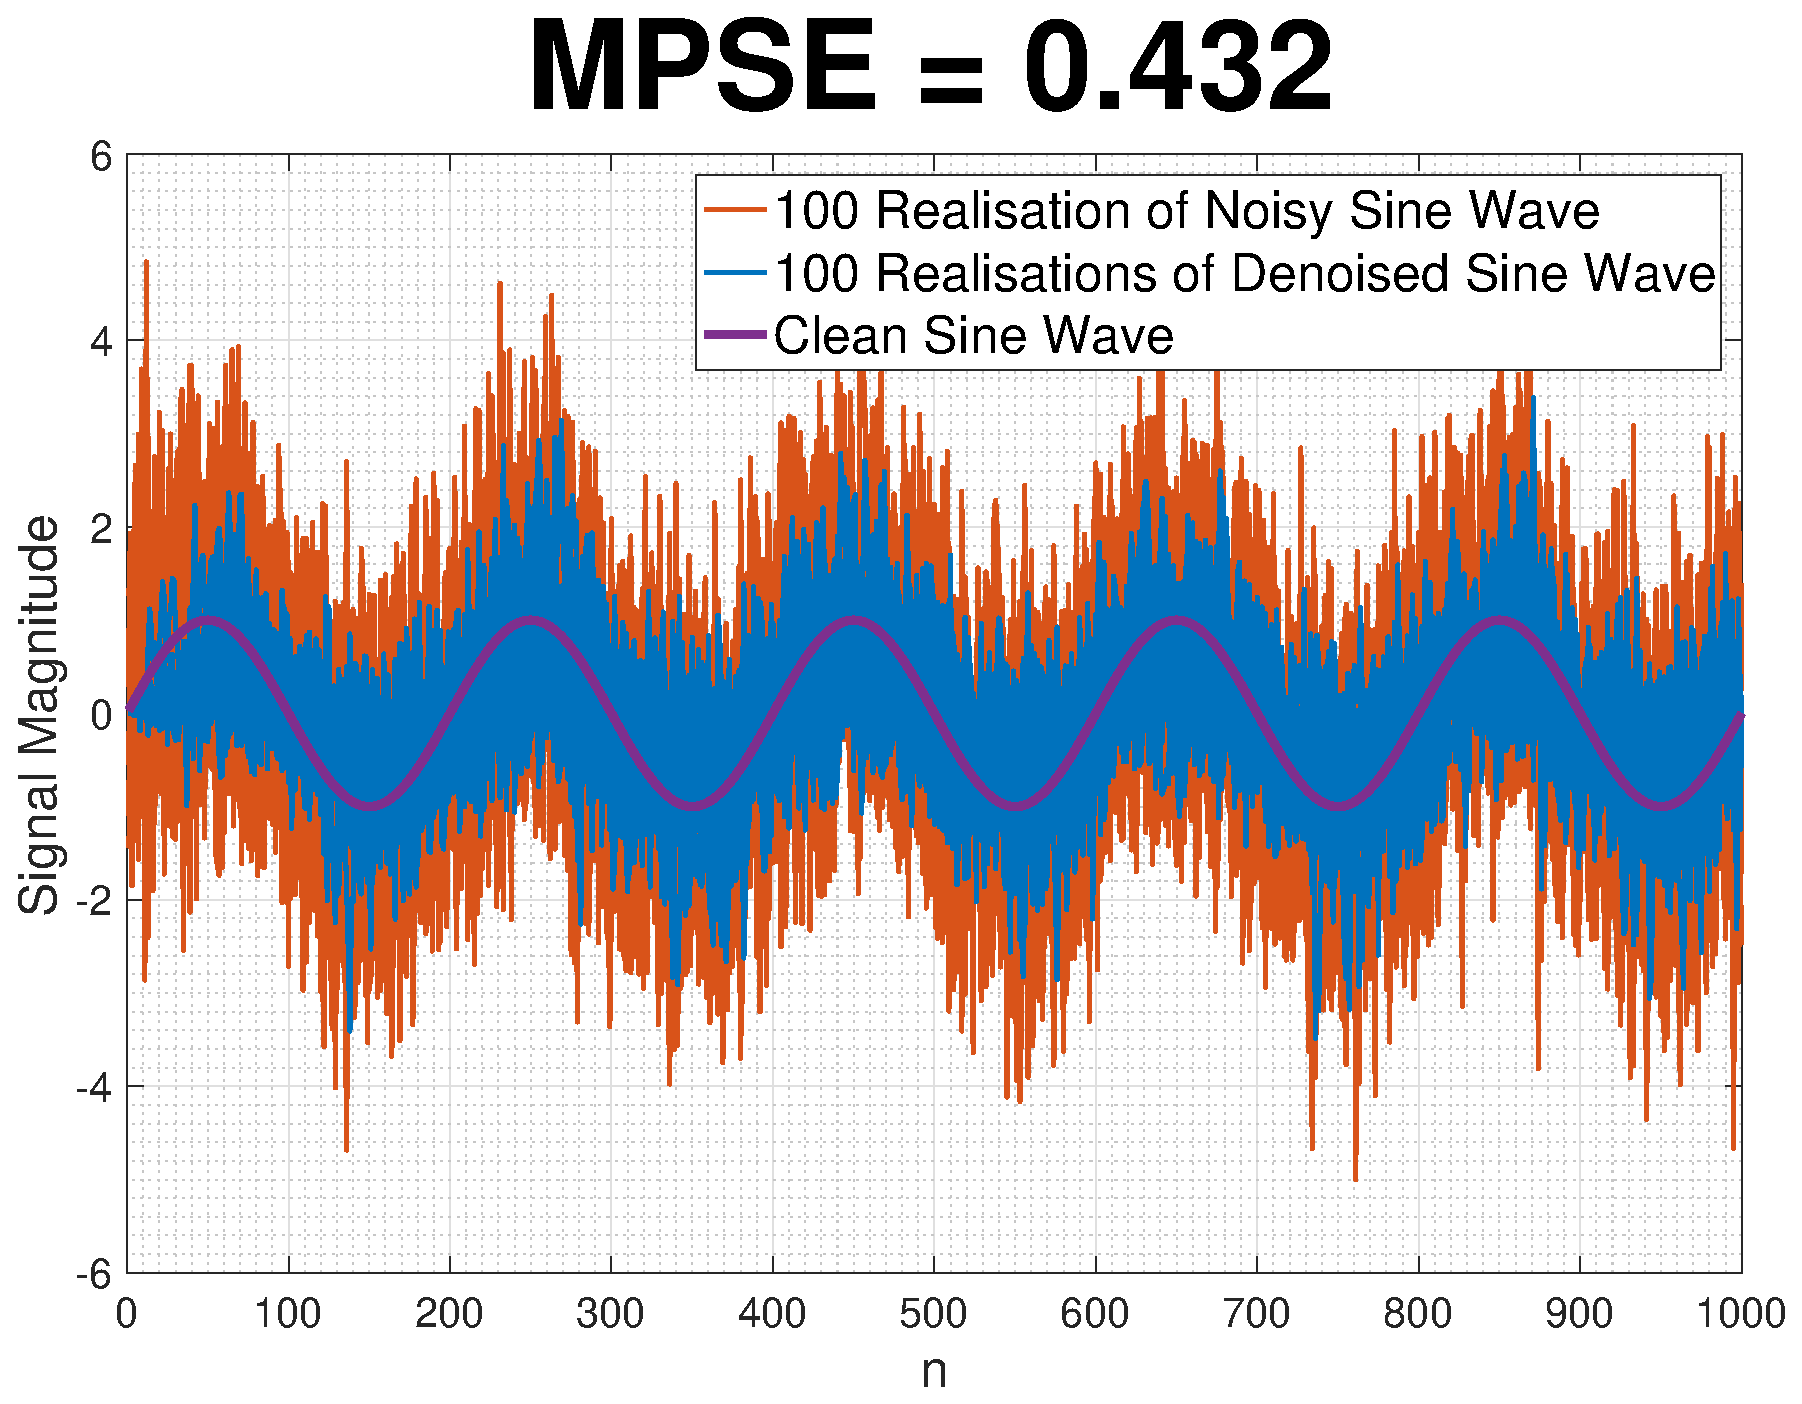
\includegraphics[width=0.24\textwidth]{part3/mpse_delay_2}
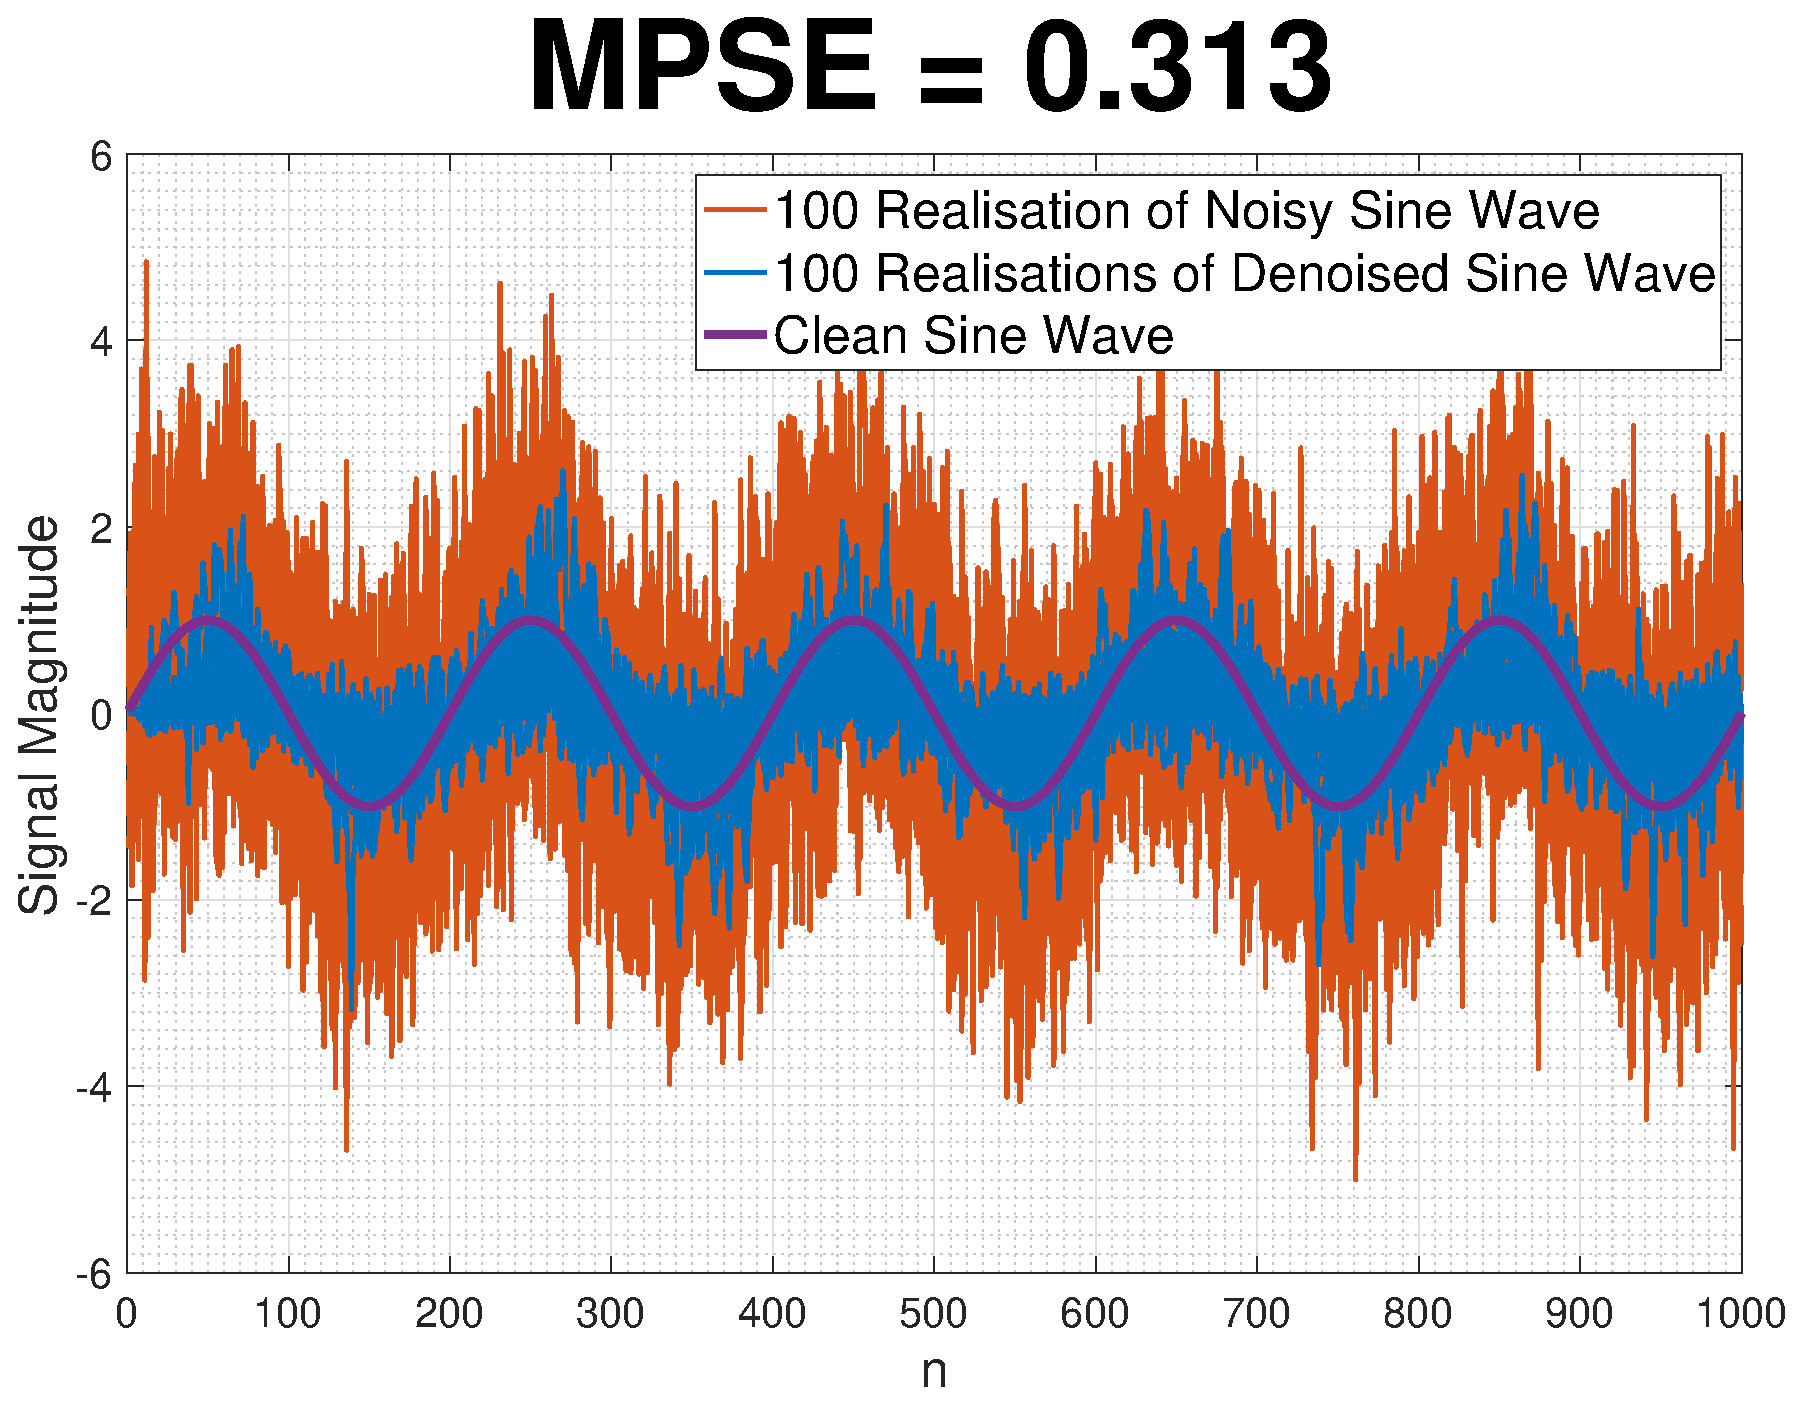
\includegraphics[width=0.24\textwidth]{part3/mpse_delay_3}
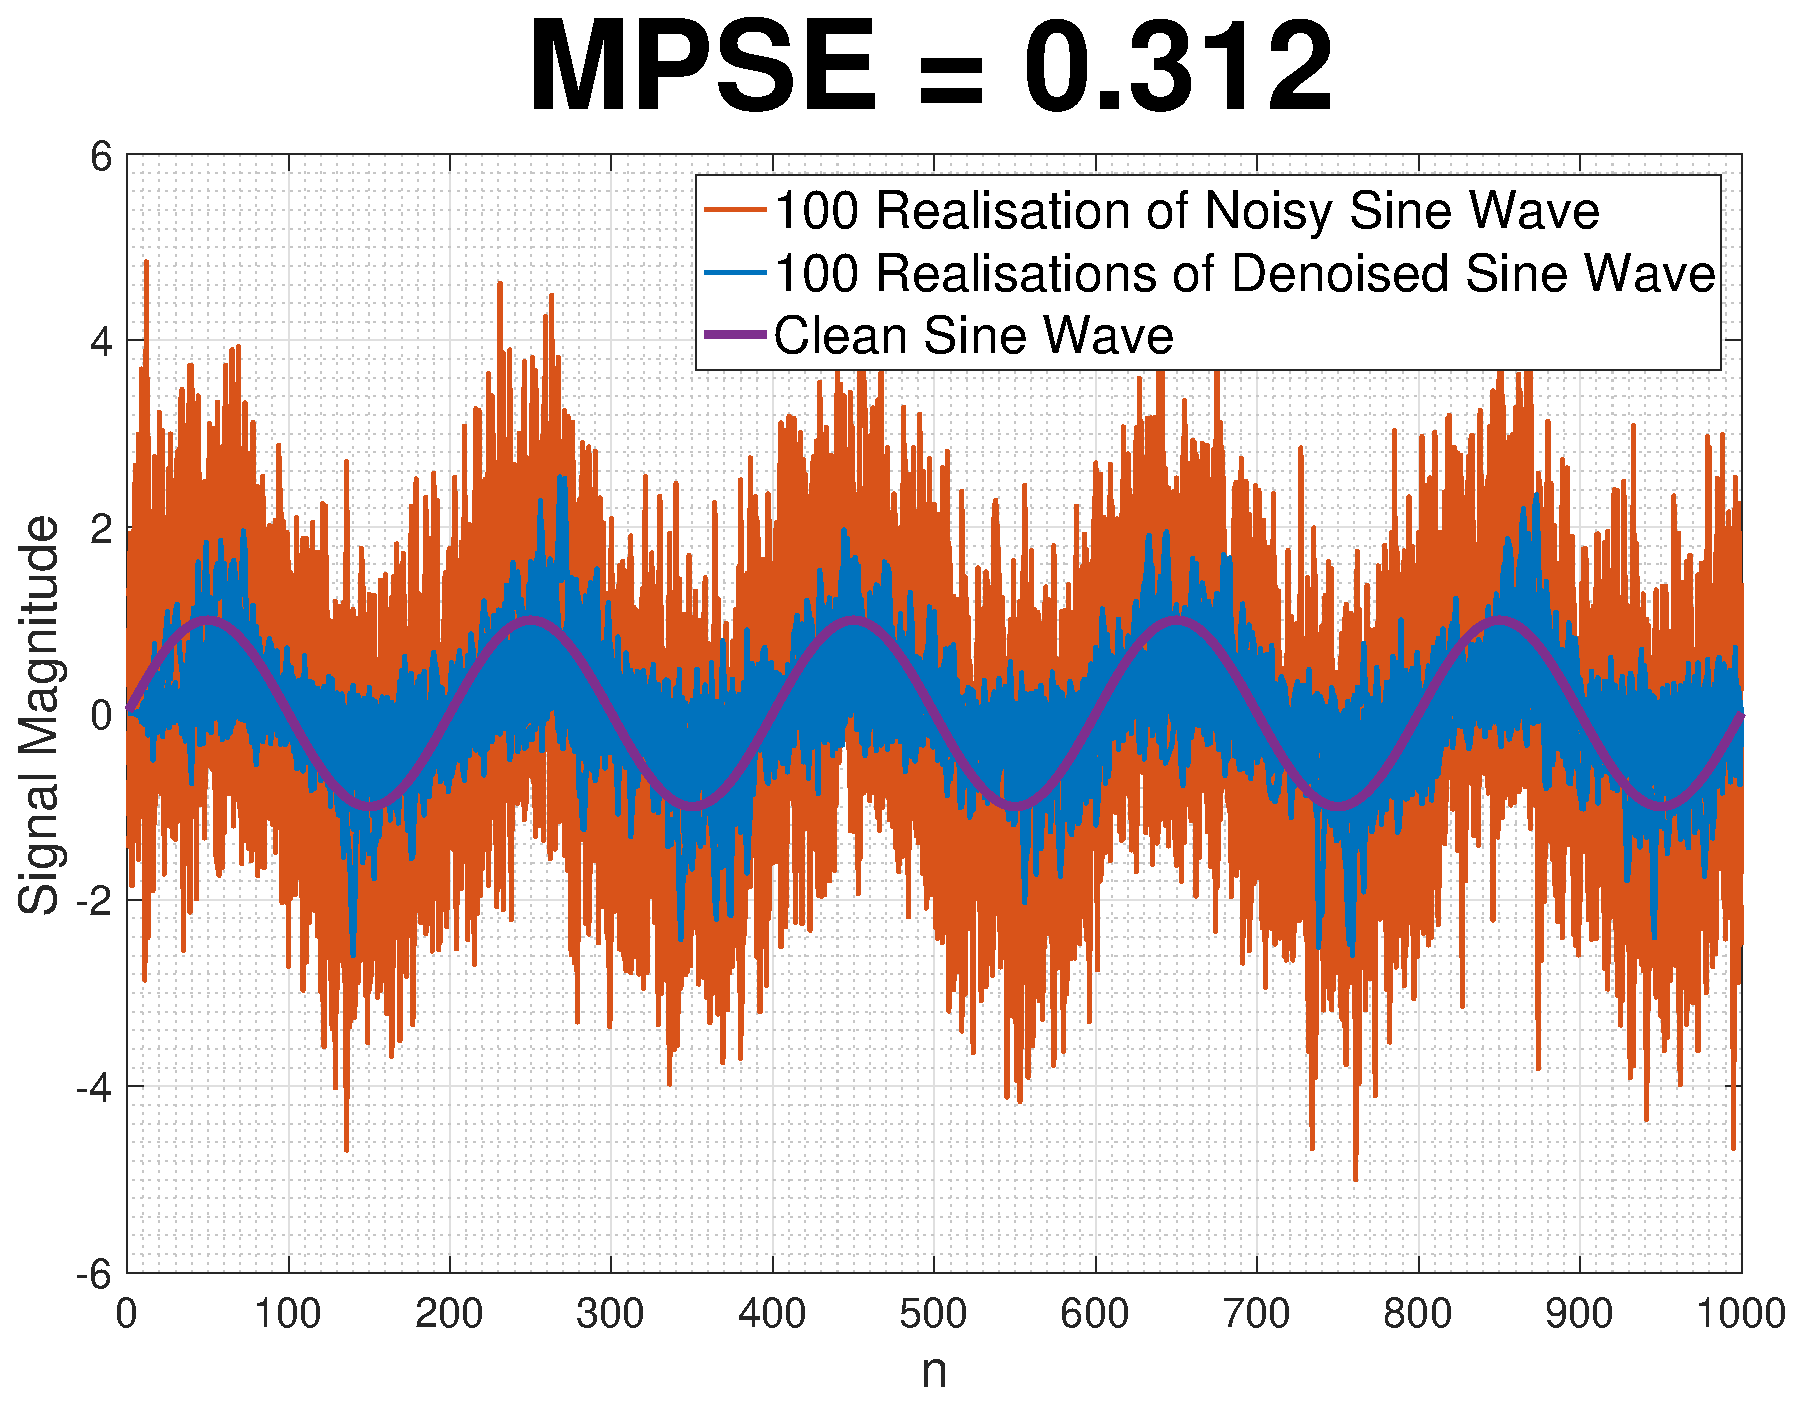
\includegraphics[width=0.24\textwidth]{part3/mpse_delay_4}
\caption{Determining Ideal Value for $\Delta$ to be used in the Adaptive Line Enhancement Algorithm}
\label{fig:ale}
\end{figure}


\noindent{}b. The results in Figure \ref{fig:ale_delay} futher verify the results above. Choosing a value of $\Delta$ greater than $2$ causes the mean-squared error to decrease for all model-orders. Note that arbitrarily increasing the value of $\Delta$ is not wise. One of the terms which contribute to the mean-squared error, $\mathbb{E}\bigg\{\bigg(s(n)-\hat{x}(n)\bigg)^2\bigg\}$, is $\mathbb{E}\bigg\{\bigg(x(n)-\hat{x}(n)\bigg)^2\bigg\}$. Increasing the value of $\Delta$ will increase the delay between $x(n)$ and $\hat{x}(n)$ and subsequently increase the mean-squared error. This effect is visualized in Figure \ref{fig:ale_delay}. Notice that the output sine-wave is shifted relatively to the ideal input sinewave when $\Delta=25$. This shift causes $\mathbb{E}\bigg\{\bigg(x(n)-\hat{x}(n)\bigg)^2\bigg\}$ to be large, thereby increasing the mean-squared error.

\begin{figure}[H]
\centering{}
\includegraphics[width=0.32\textwidth]{part3/delay_vs_mpse}
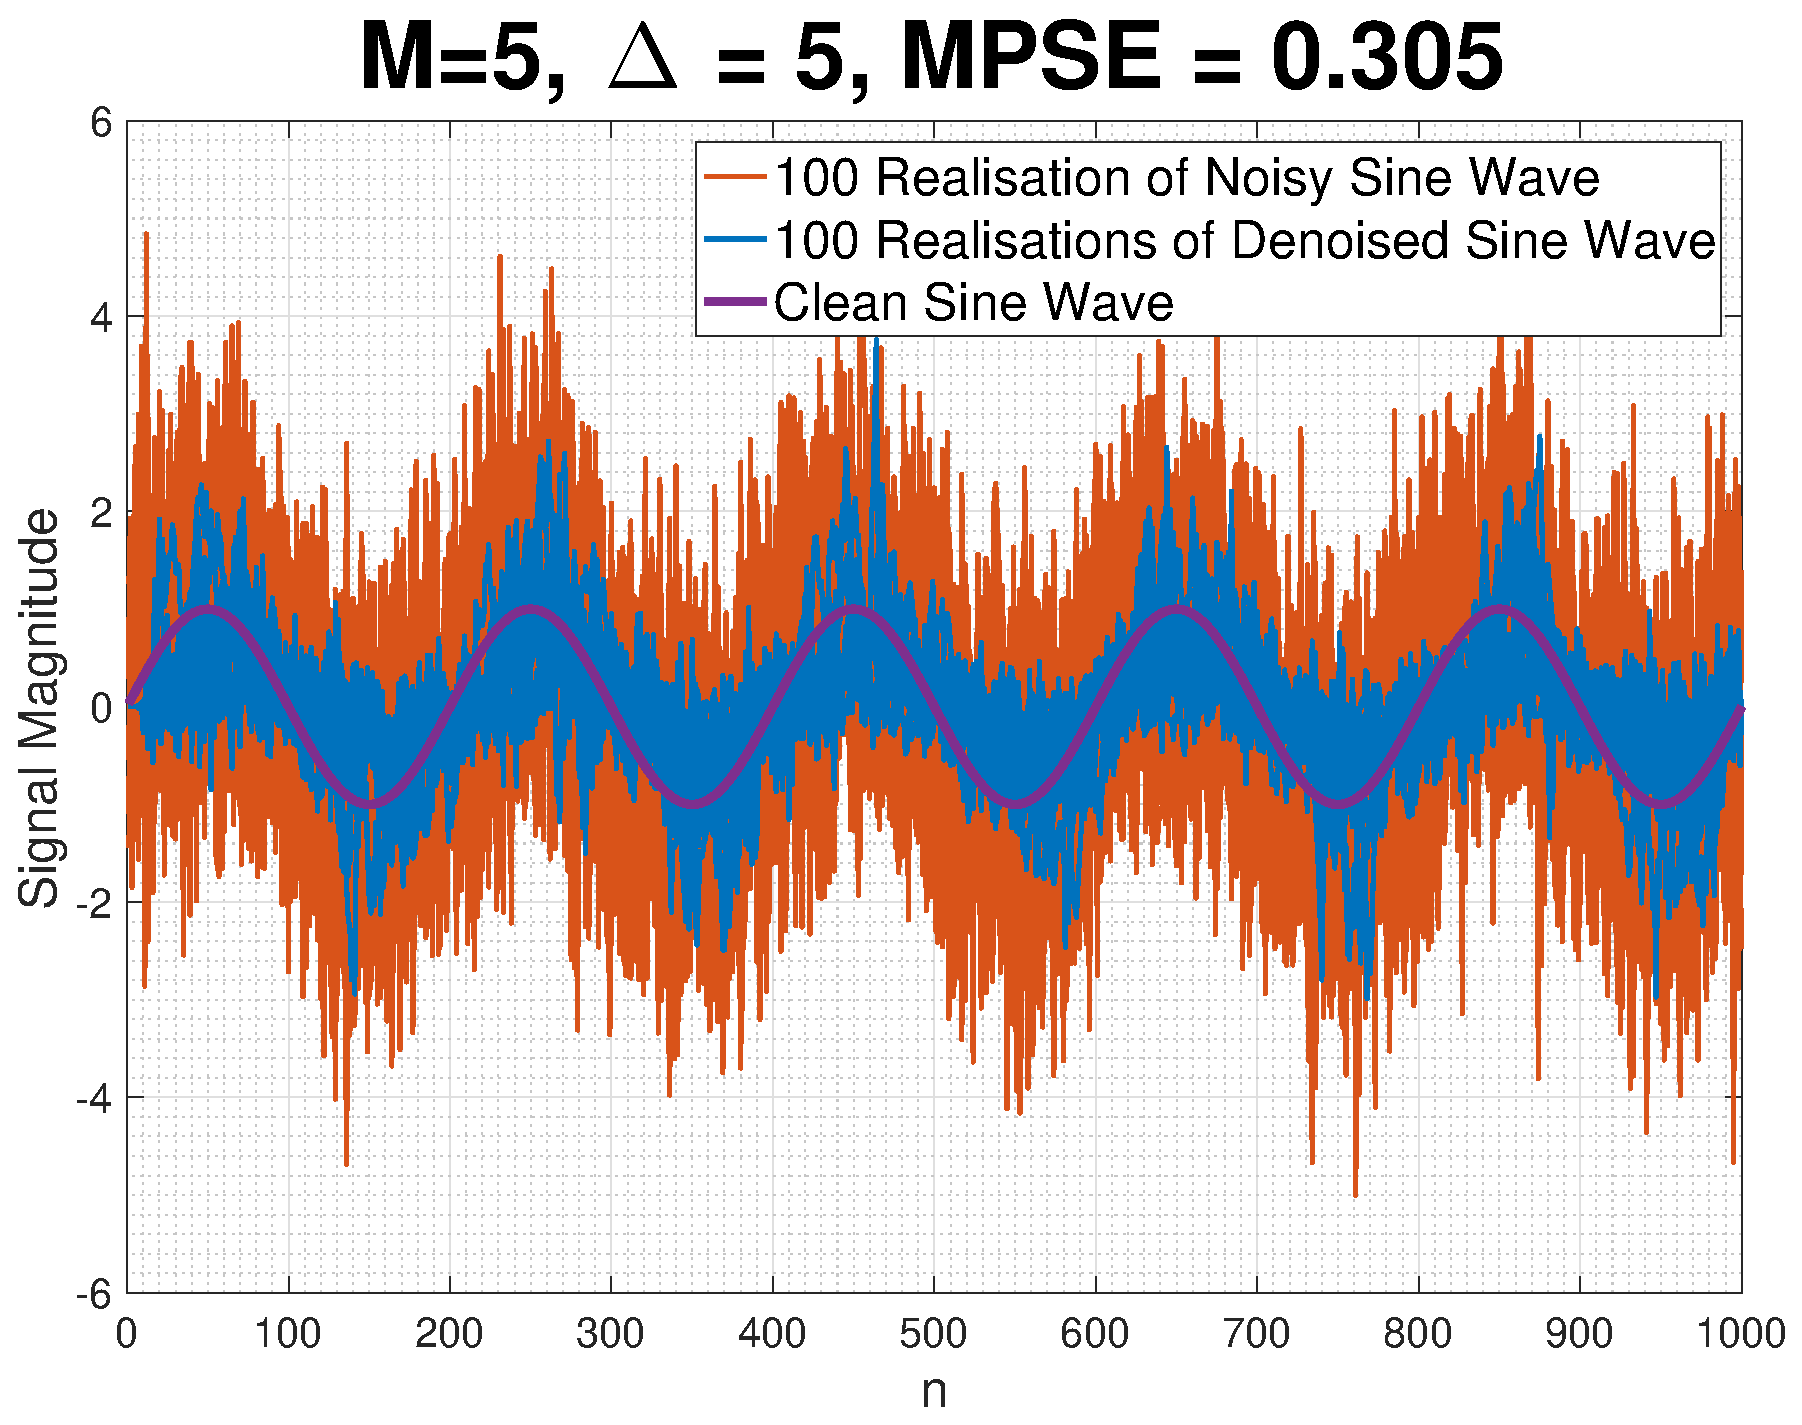
\includegraphics[width=0.32\textwidth]{part3/mpse_delay_5}
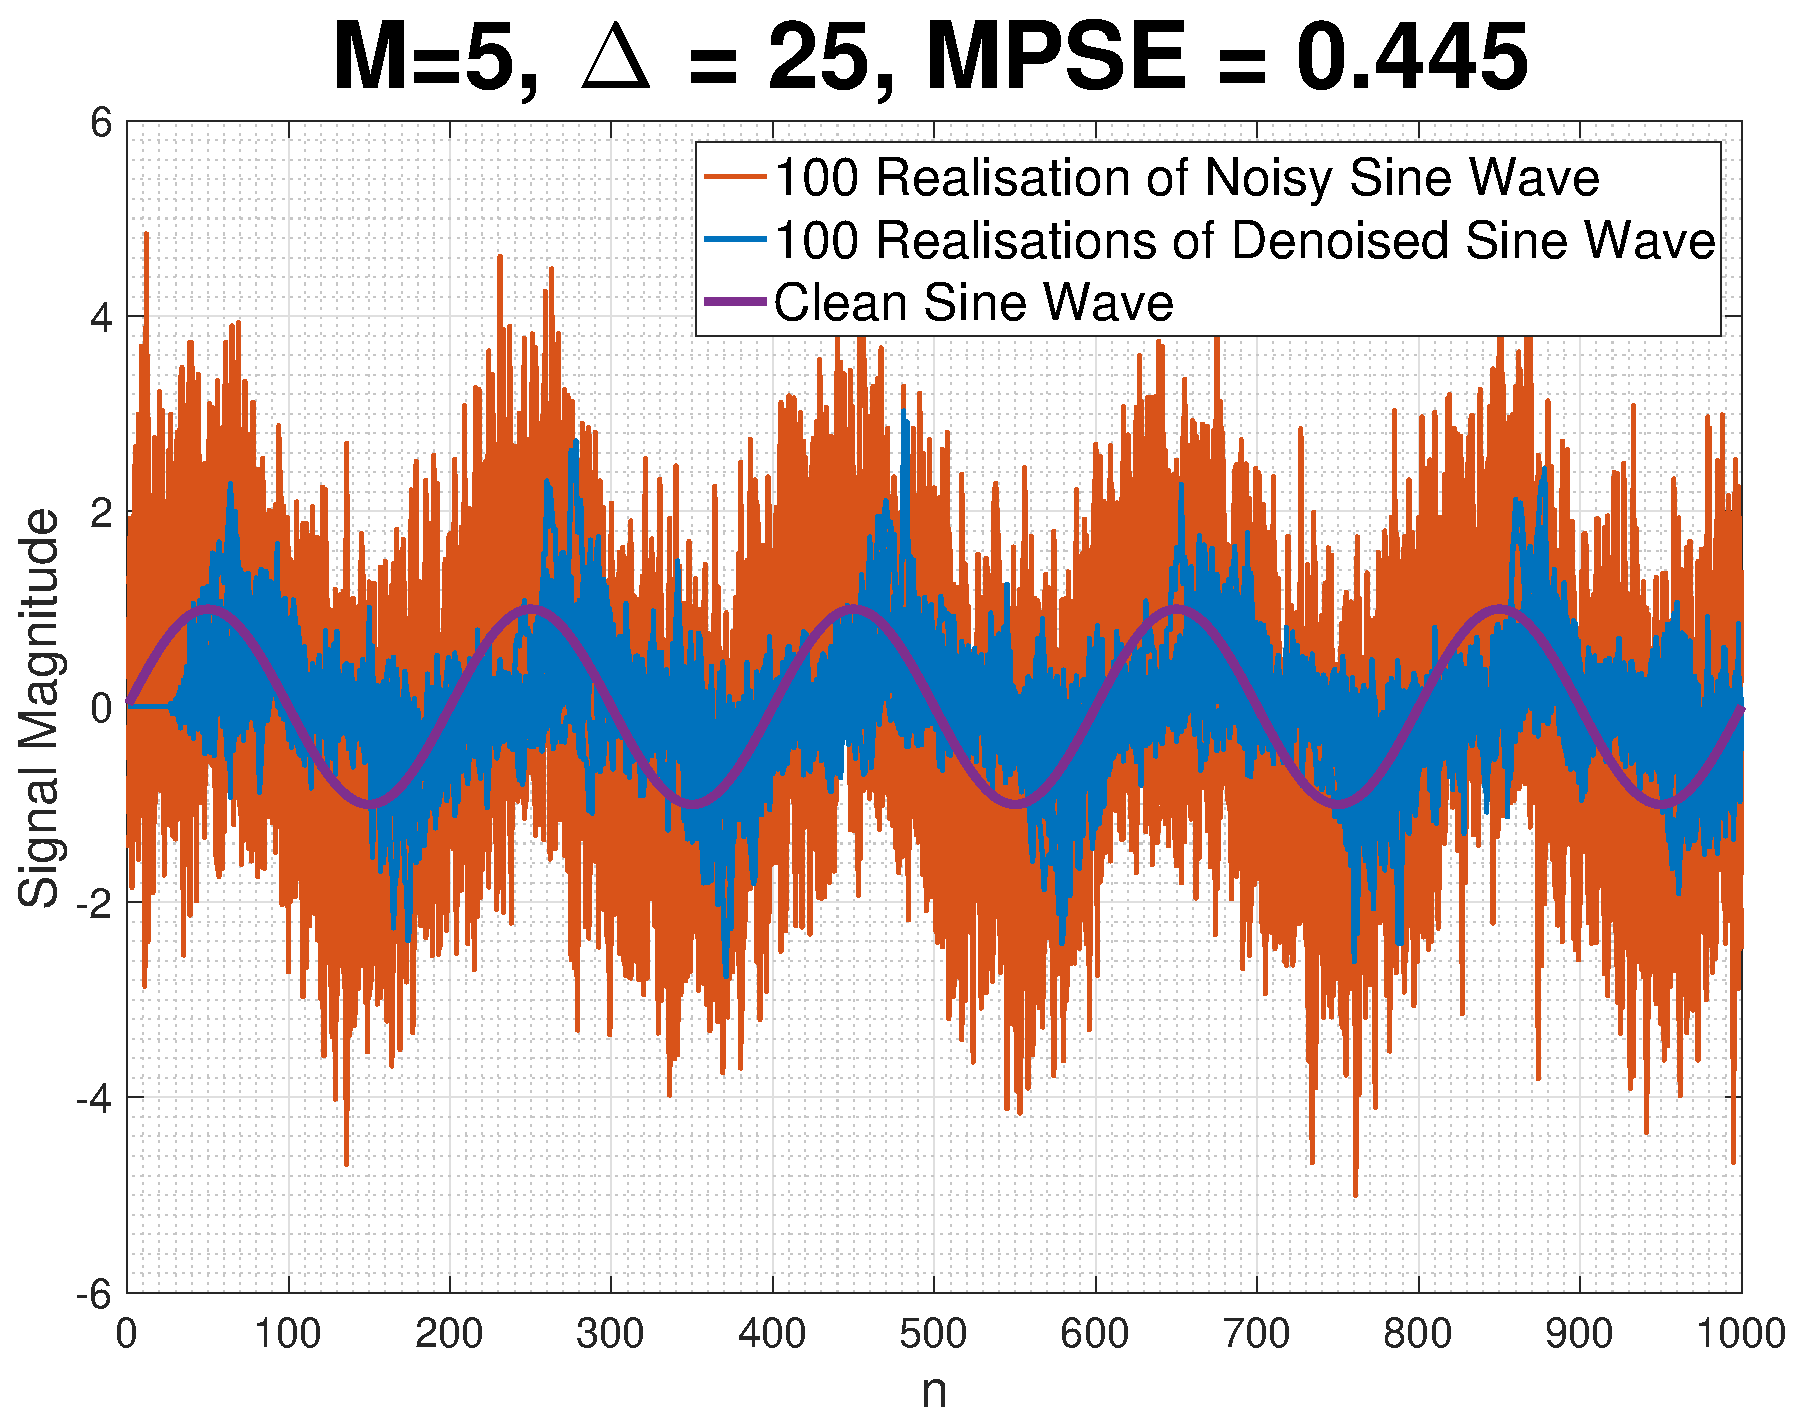
\includegraphics[width=0.32\textwidth]{part3/mpse_delay_25}
\caption{Studying the Effects of Increasing Delay on the MPSE}
\label{fig:ale_delay}
\end{figure}


\noindent{}Theoretically, a higher model-order should be able to describe the highly periodic process with greater accuracy. However, since we are deriving the solution numerically, factors such as convergence, stability and computational complexity should also be taken into account. Note increasing the model order, while keeping $\mu$ constant may result in an increase in the mean-squared error. This effect is observed for values of $M>6$. It is possible to keep $\mu$ small and increase the model order however this would cause the algorithm to converge slowly. Analyzing Figure \ref{fig:ale_model}, a pragmatic choice is to set $M=6$ and set $\mu=0.005$.

\begin{figure}[H]
\centering{}
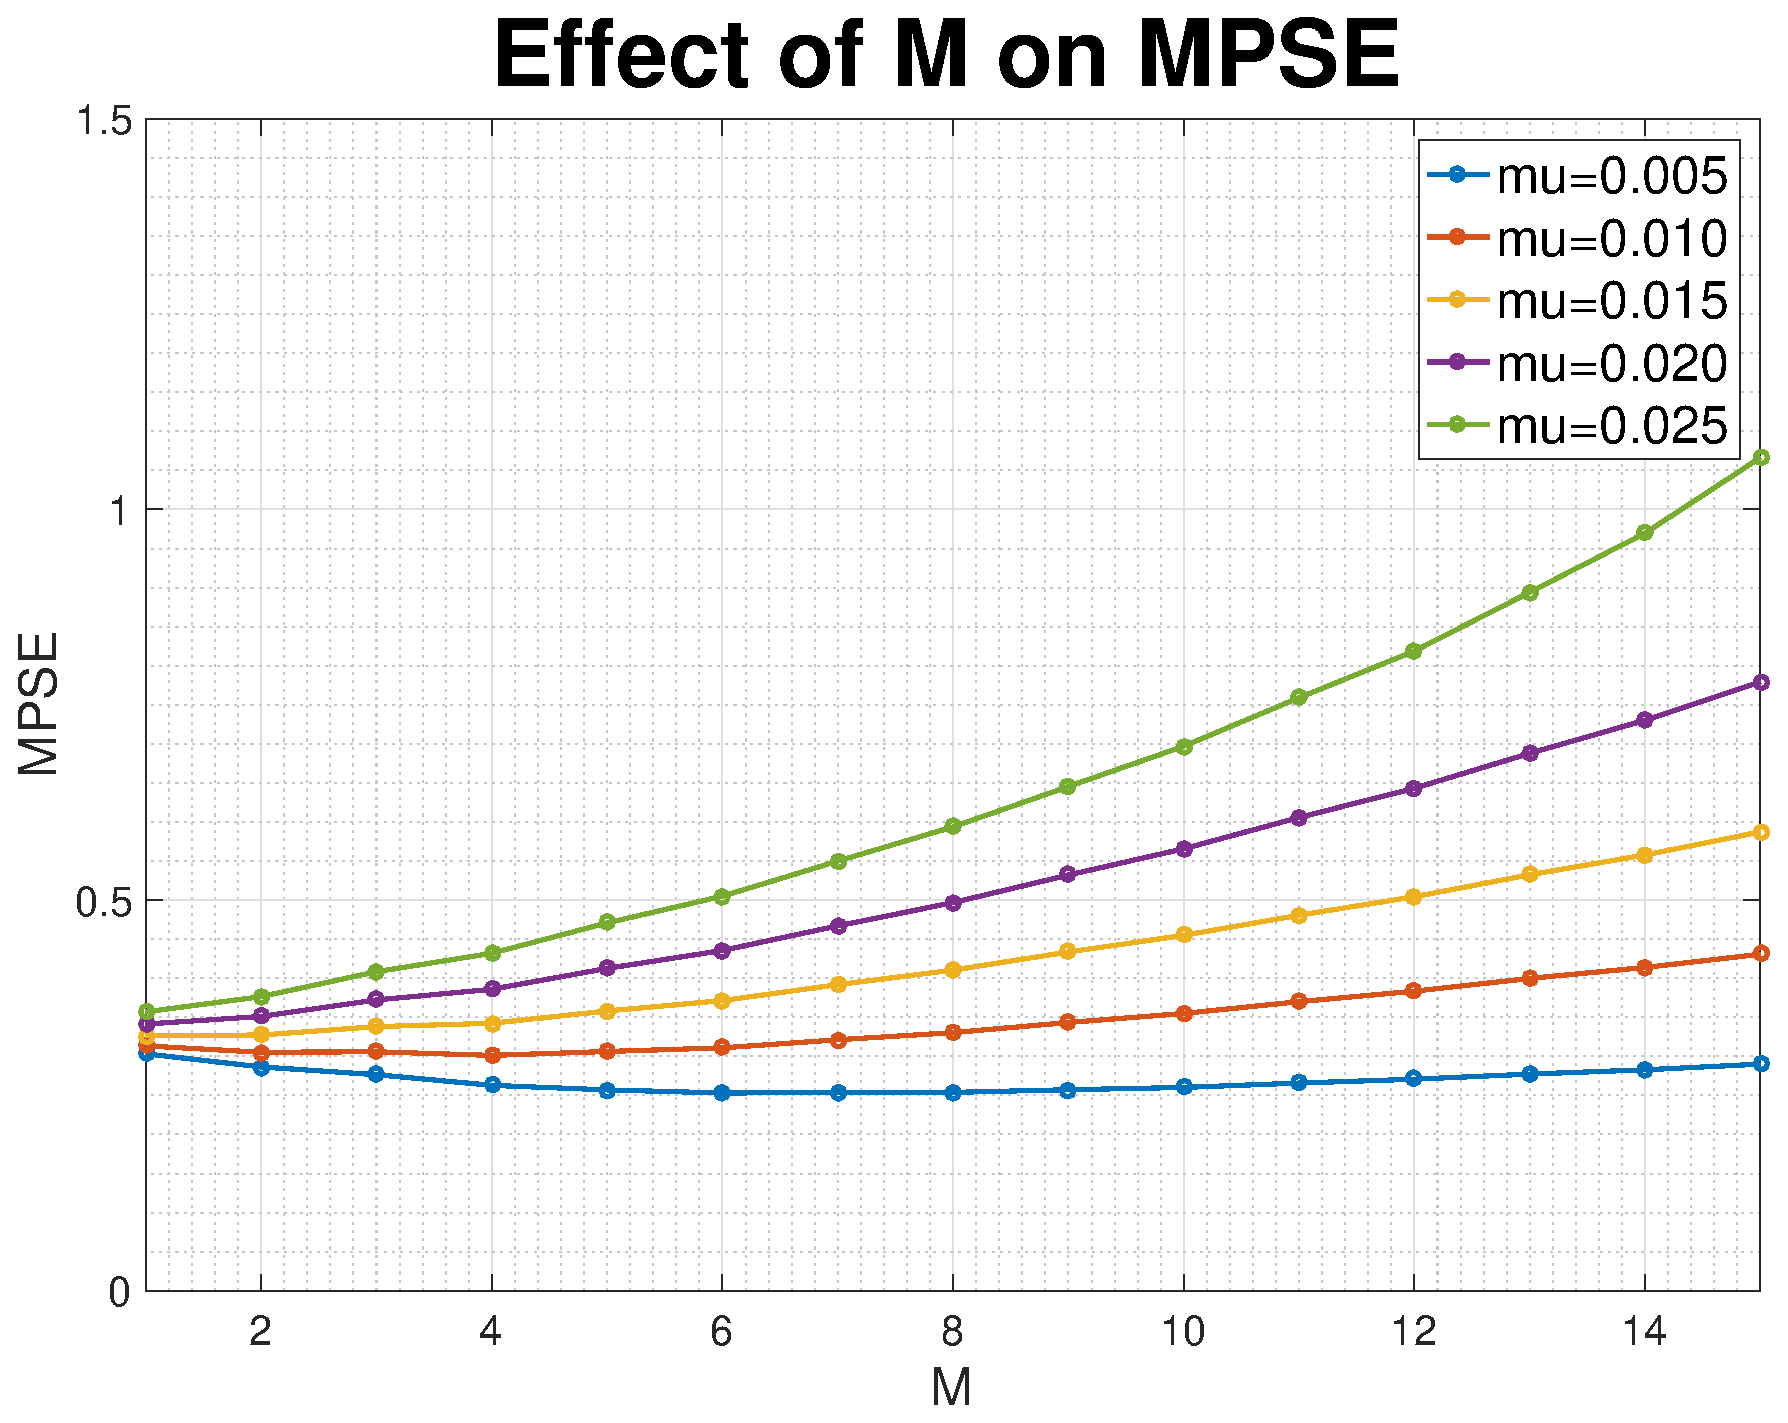
\includegraphics[width=0.32\textwidth]{part3/model_order_mpse}
\caption{Studying the Effects of Increasing Model Order on the MPSE}
\label{fig:ale_model}
\end{figure}

\noindent{}c. The performance of the ALE configuration and the Adaptive Noise Cancellation (ANC) configuration are compared in the figure below. It is clear that the ANC configuration performs significantly better, once it has converged. However, notice that for small values of $n$, the ANC configuration incurs large errors.

\begin{figure}[H]
\centering{}
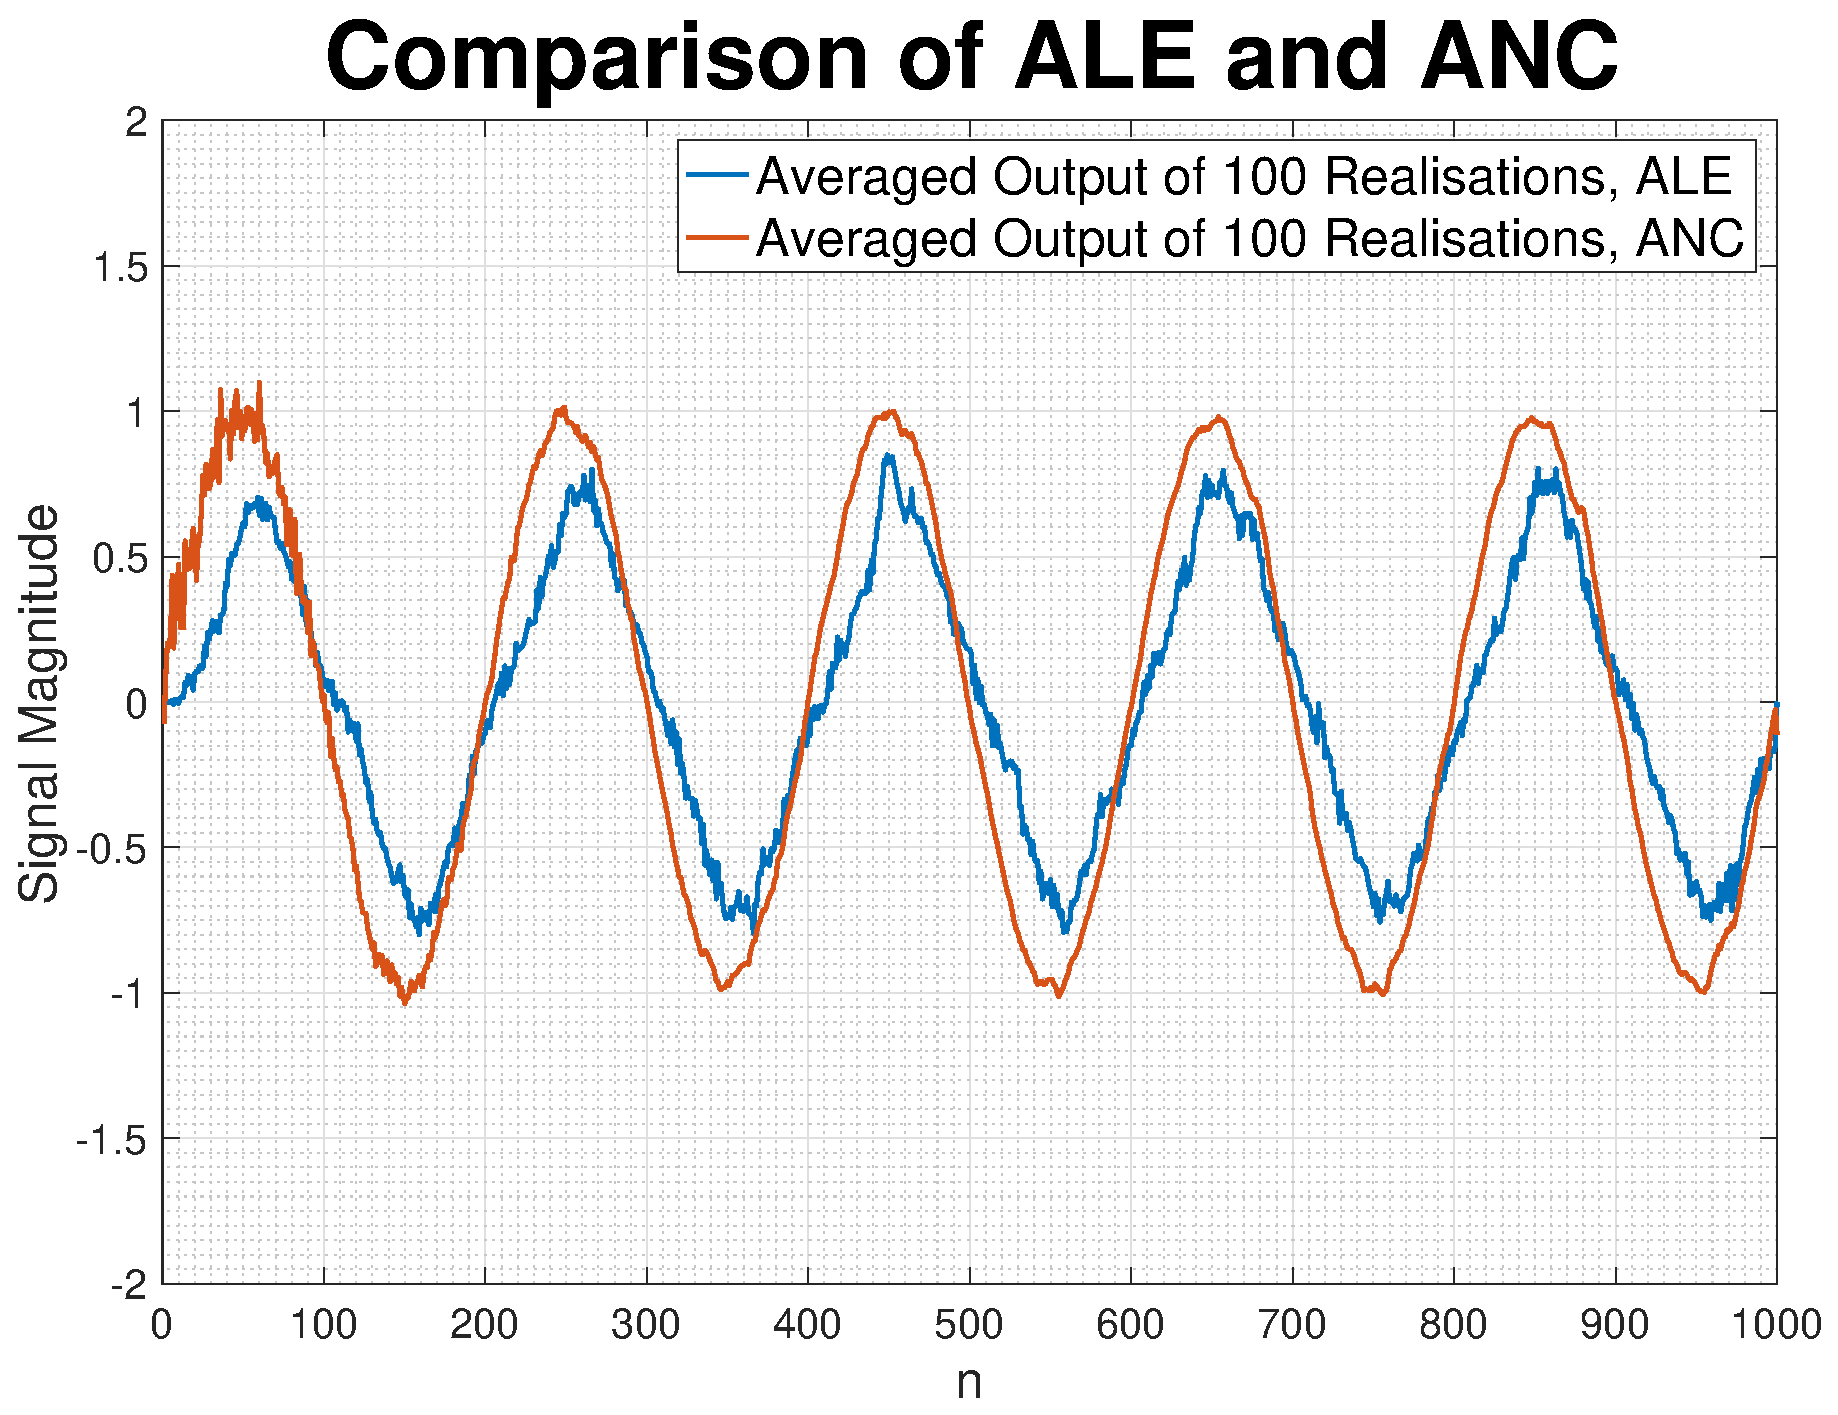
\includegraphics[width=0.32\textwidth]{part3/anc_ale_comparison}
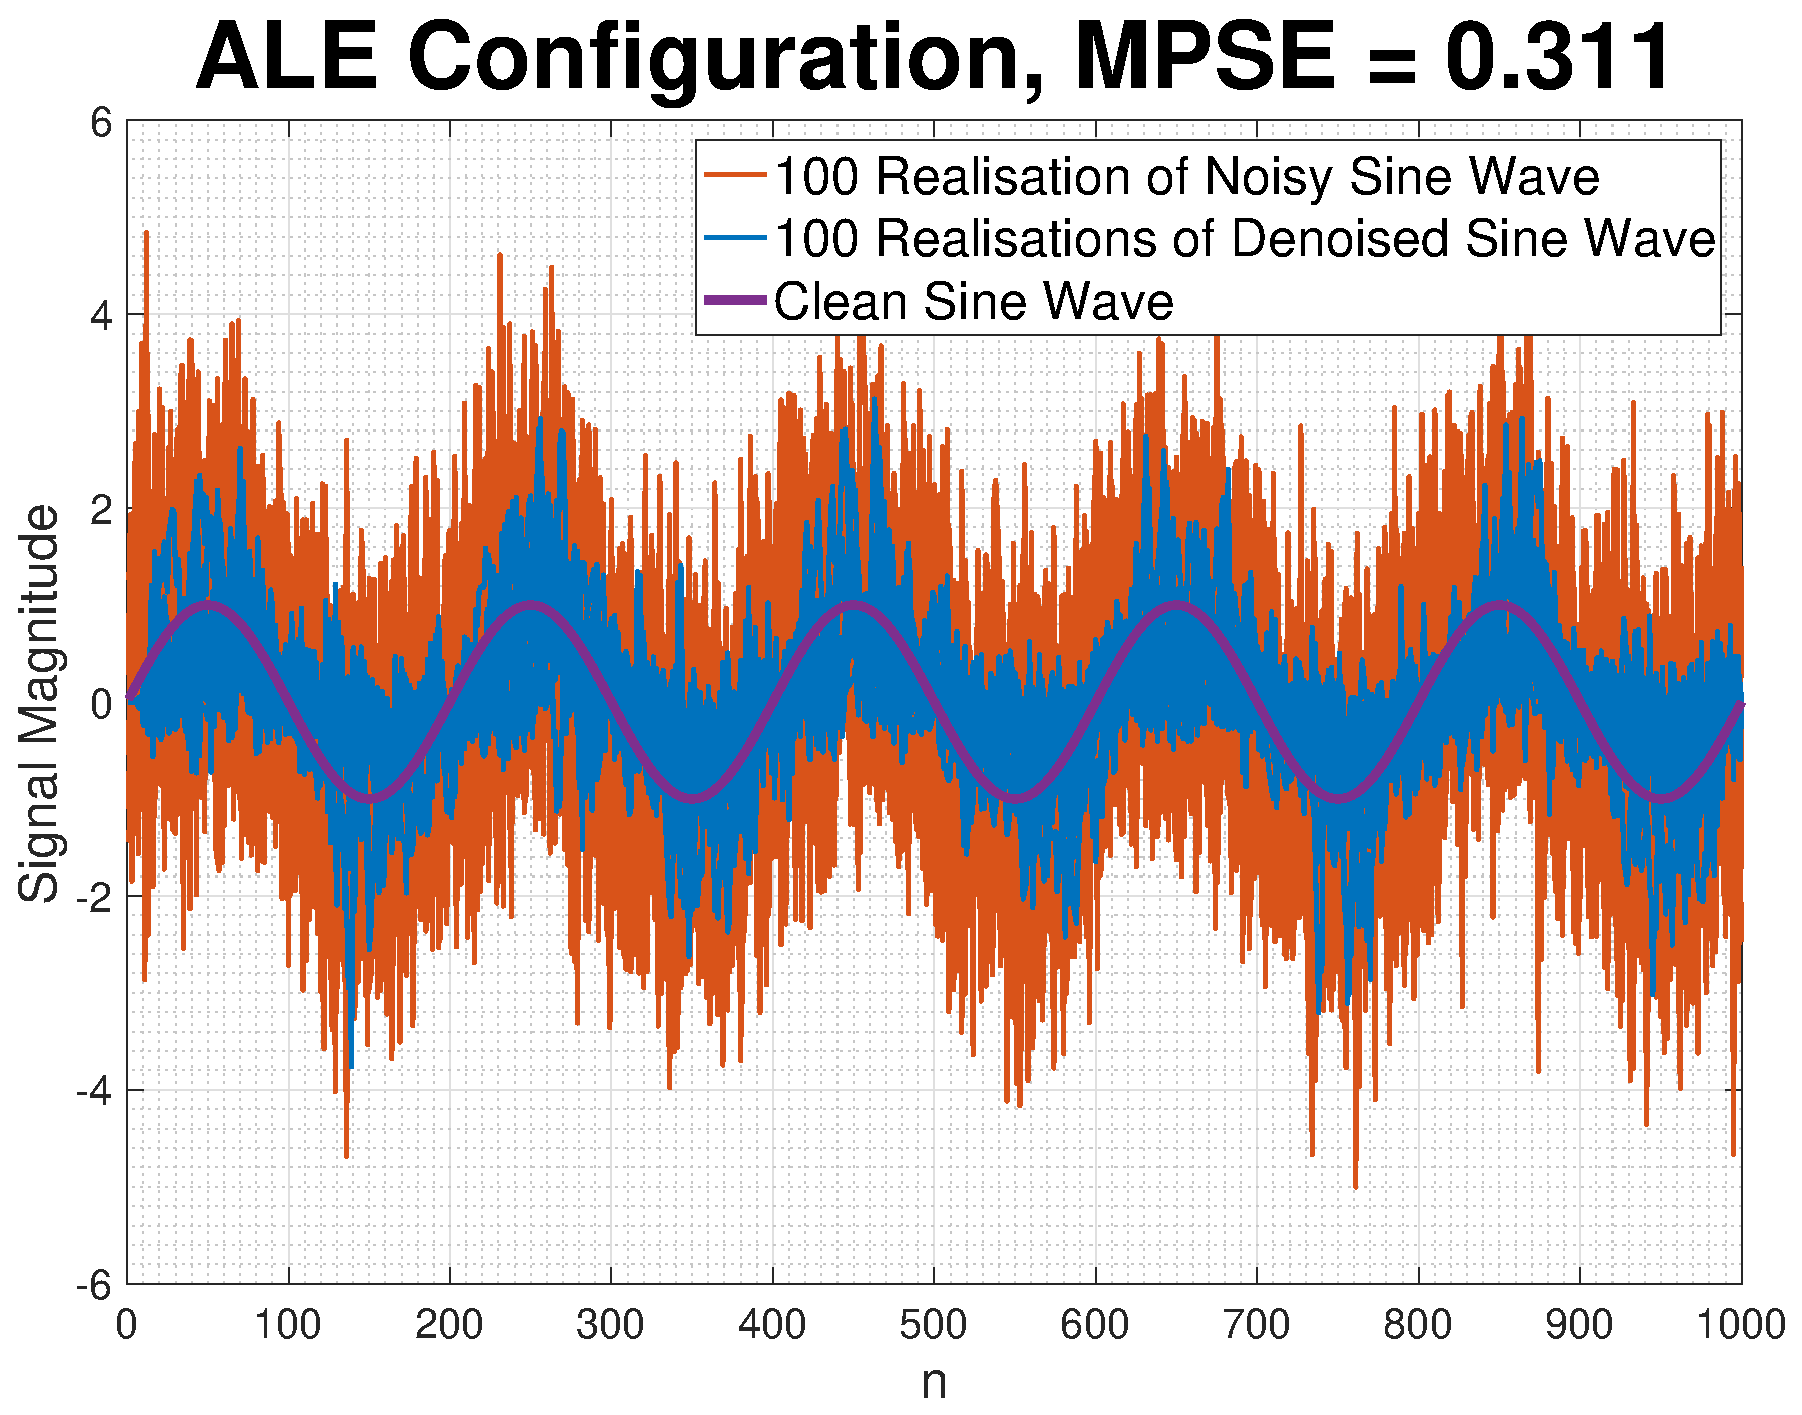
\includegraphics[width=0.32\textwidth]{part3/ale_mpse}
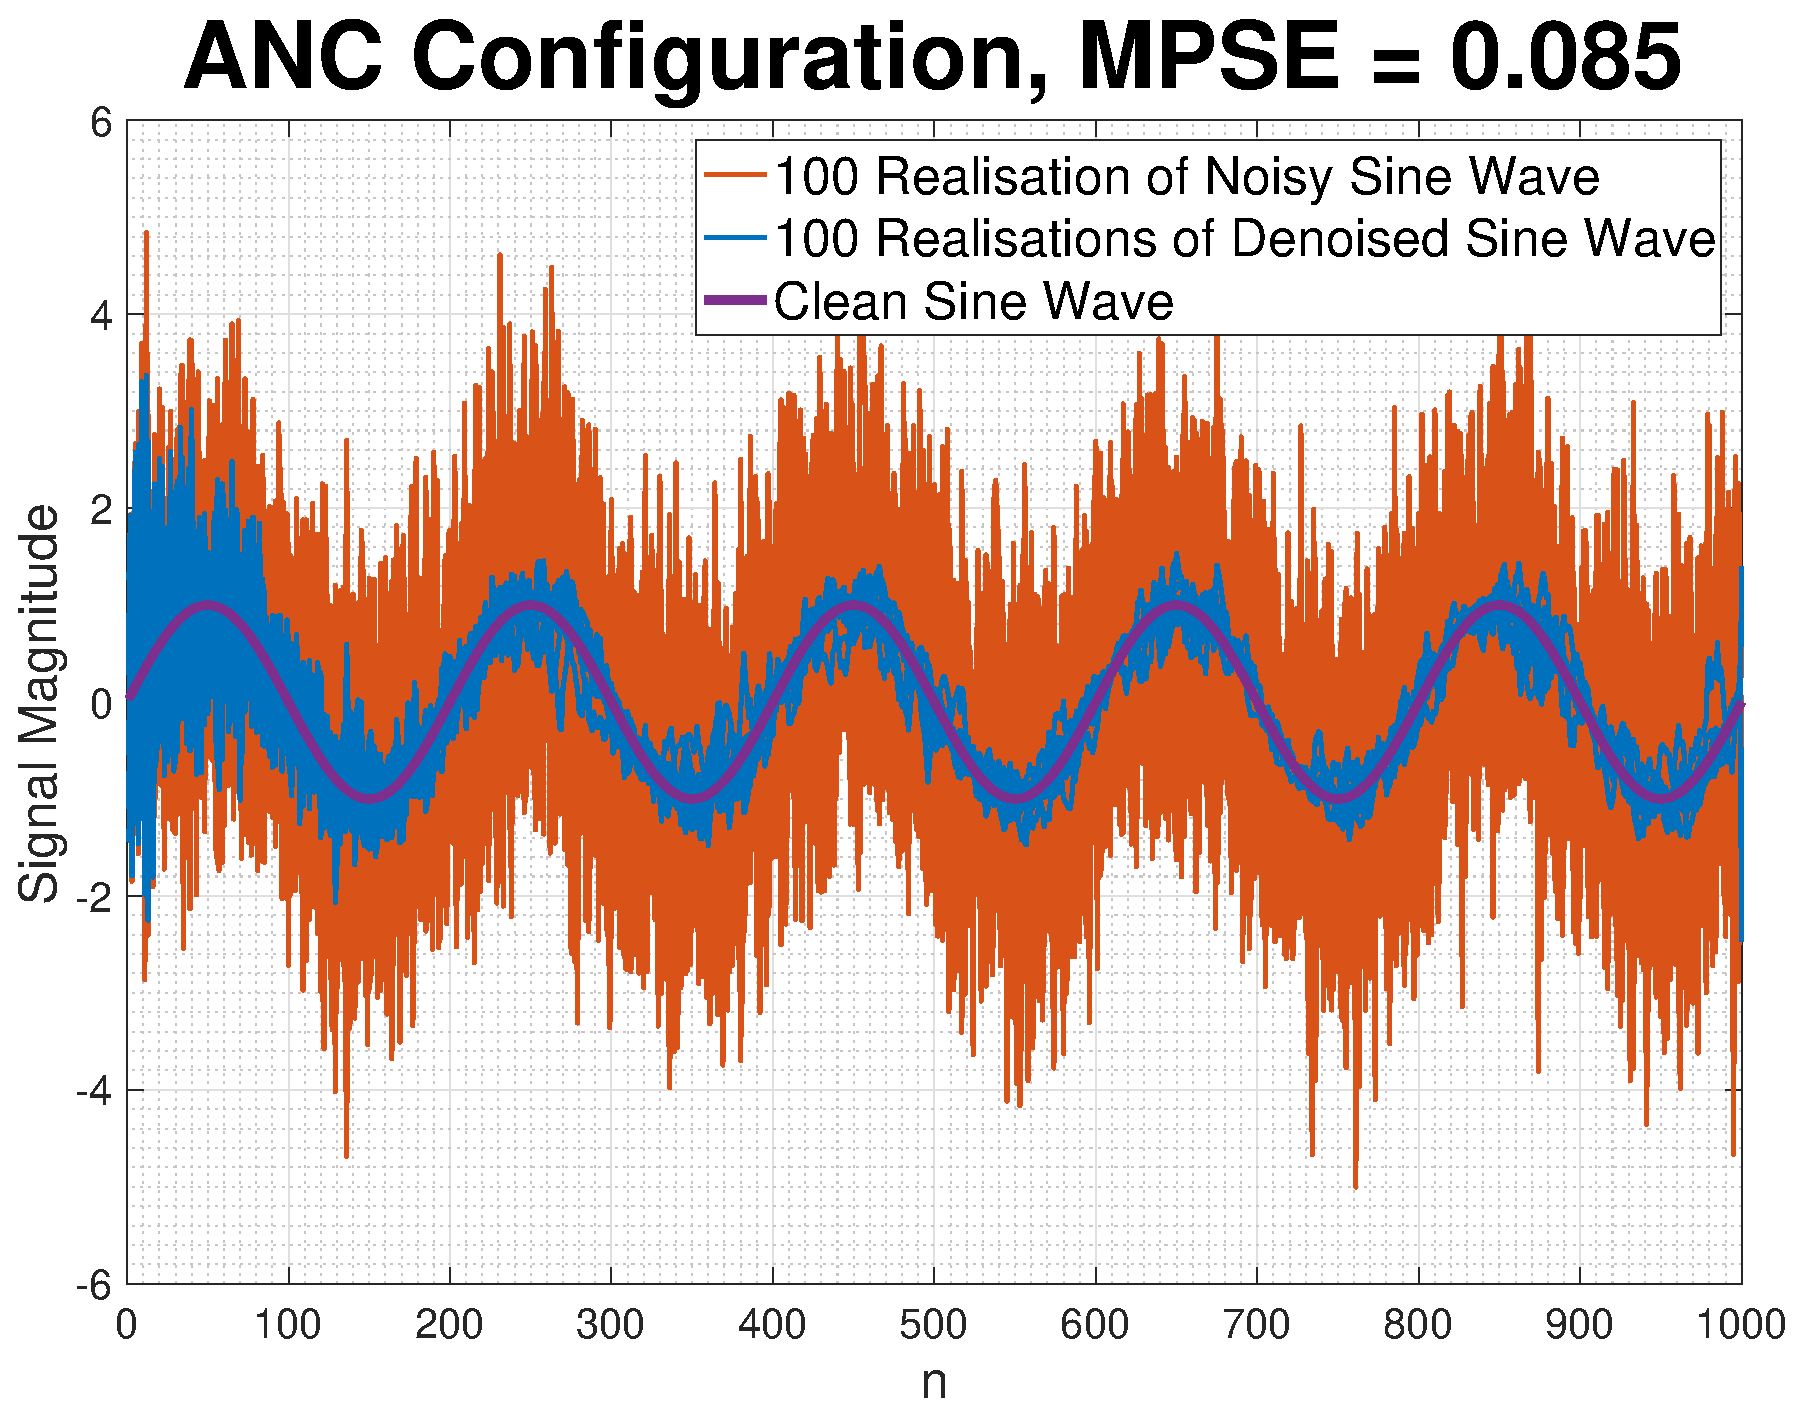
\includegraphics[width=0.32\textwidth]{part3/anc_mpse}
\caption{Comparison of ALE and ANC Configurations for Denoising Sinewave}
\end{figure}

\noindent{}d. The spectrogram in Figure \ref{fig:ref_spect} is graphed for reference. It shows the original EEG data with a very strong component at 50 Hz. The length of each segment is $4096$, with an $80\%$ overlap between segments. Also, each segment is windowed with a Hamming window. 

\begin{figure}[H]
\centering{}
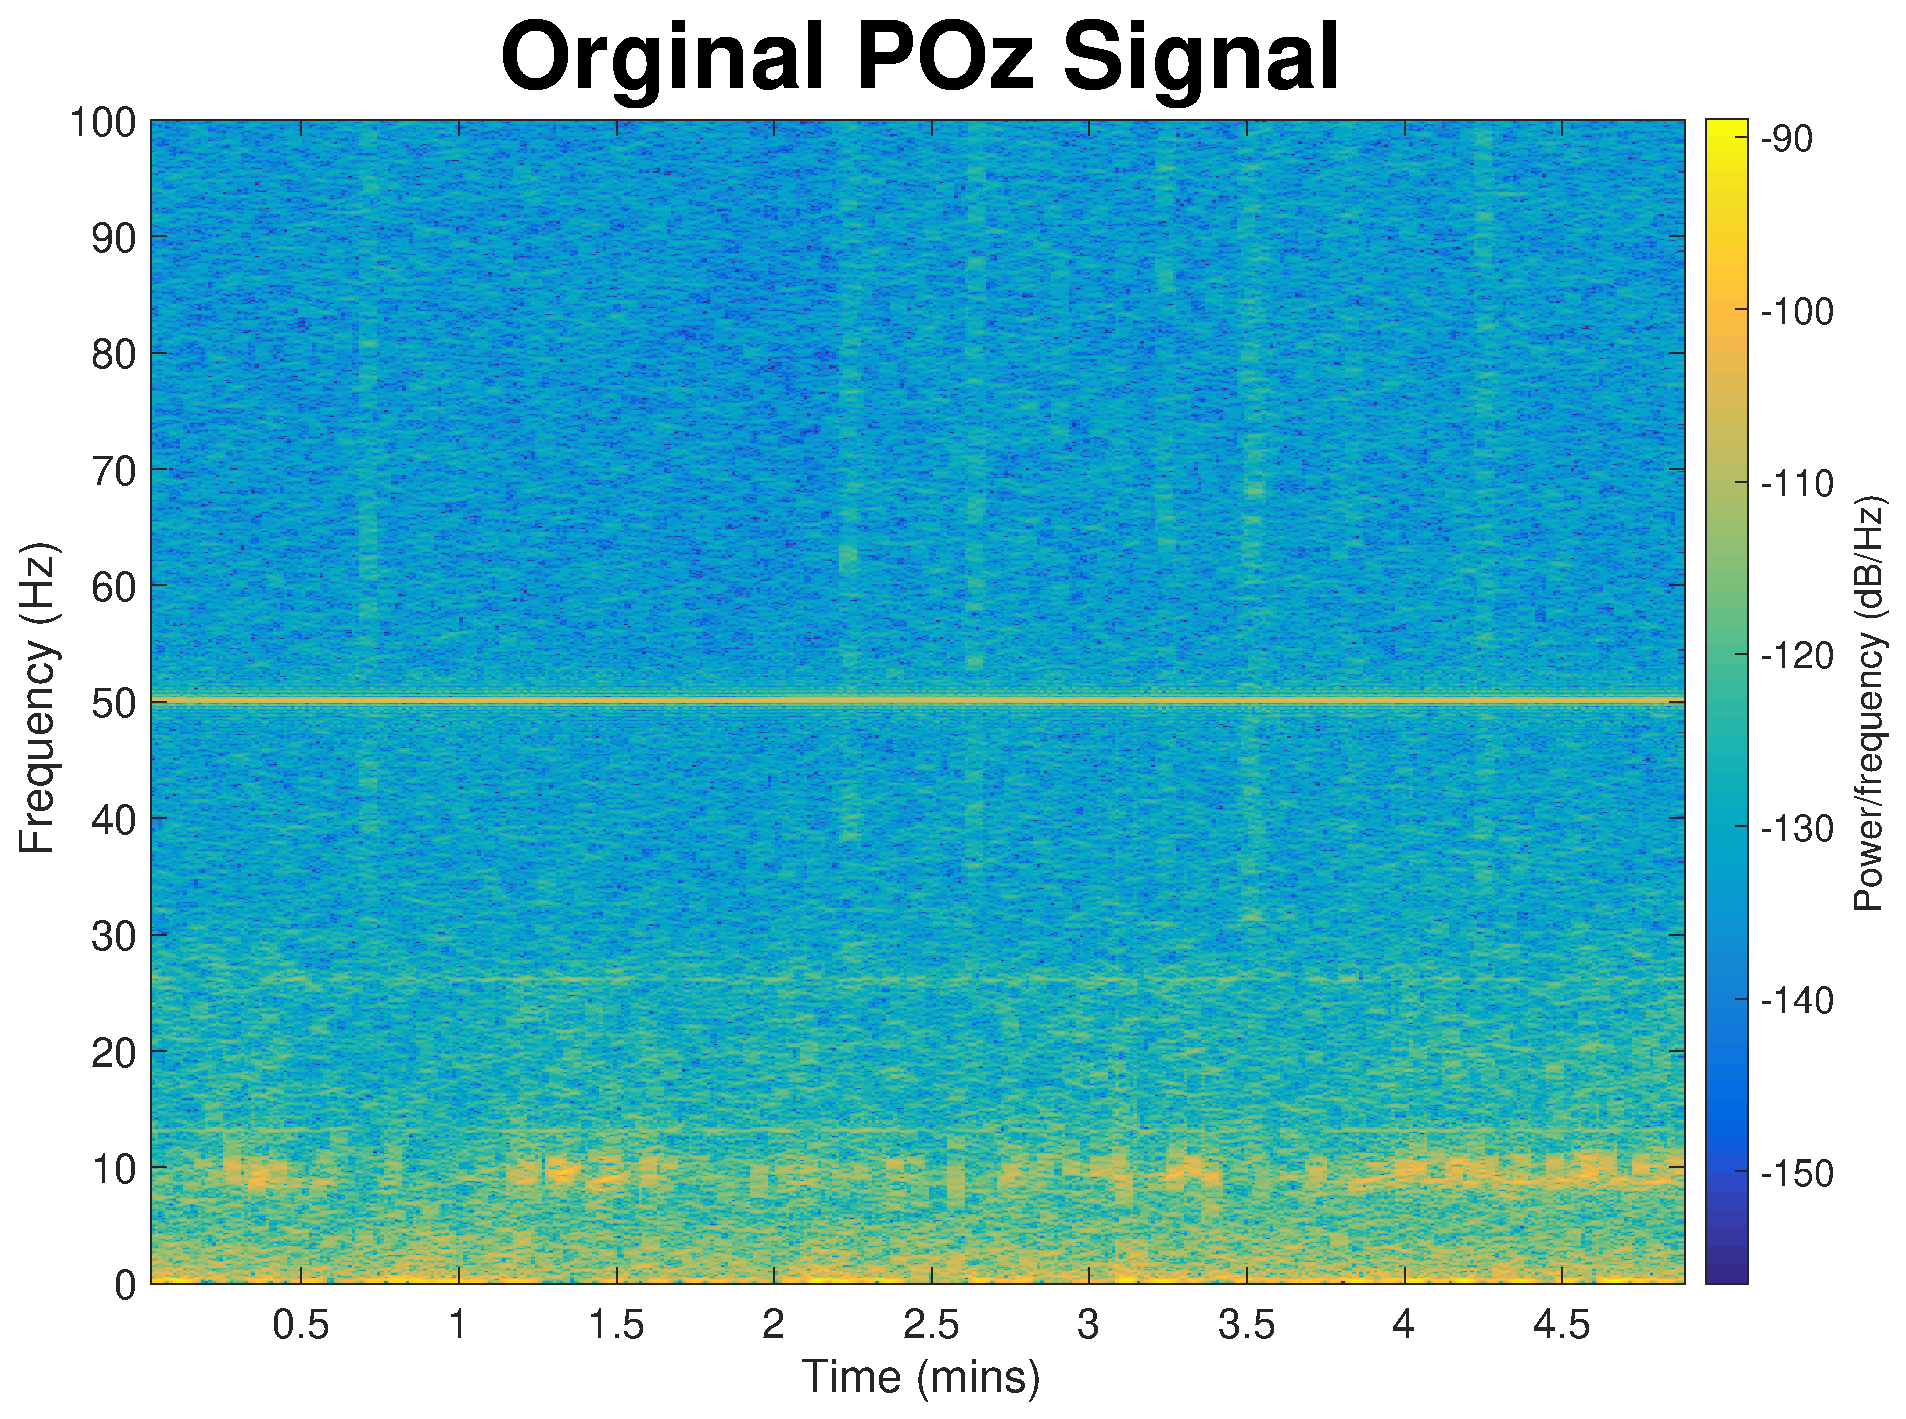
\includegraphics[width=0.32\textwidth]{part3/original_POz_spectrogram}
\caption{Original EEG Data collected from POz Location on the Scalp with Strong Component at 50 Hz}
\label{eq:ref_spect}
\end{figure}

\noindent{}The first step is to determine the value of $M$ that will remove the strong 50 Hz component. The figure below shows the effect of increasing the model order. Increasing the model order results in a filter that is more efficient at removing the noise. However, notice that certain artifacts have started to occur. With $M=25$ and $\mu=0.01$, the filter is not only removing the 50 Hz component but it is also suppressing components between 40 Hz and 60 Hz.

\begin{figure}[H]
\centering{}
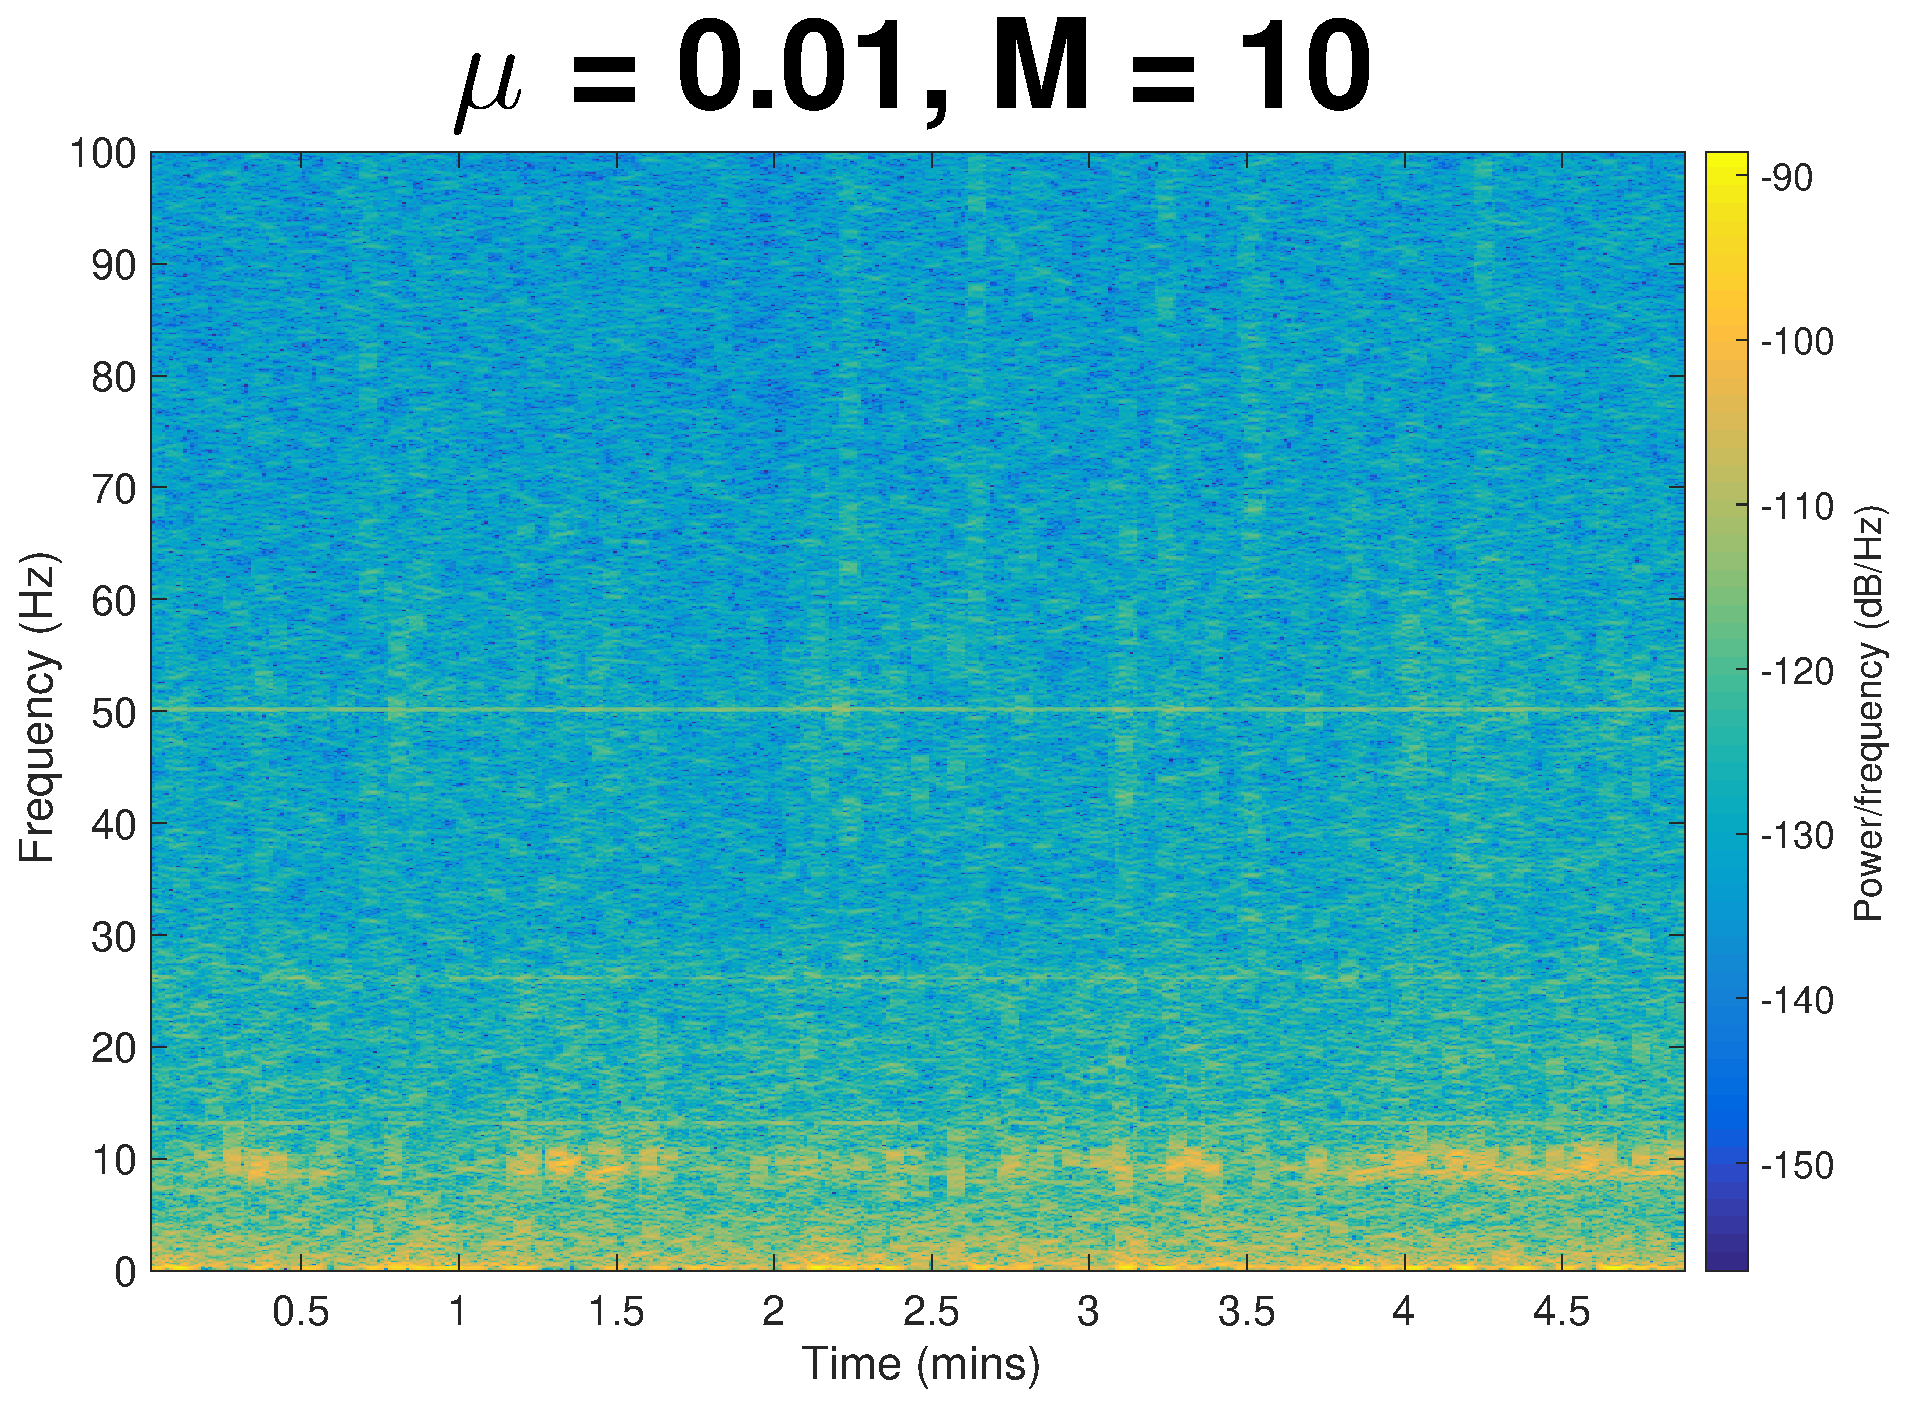
\includegraphics[width=0.24\textwidth]{part3/POz_mu_01_M_10}
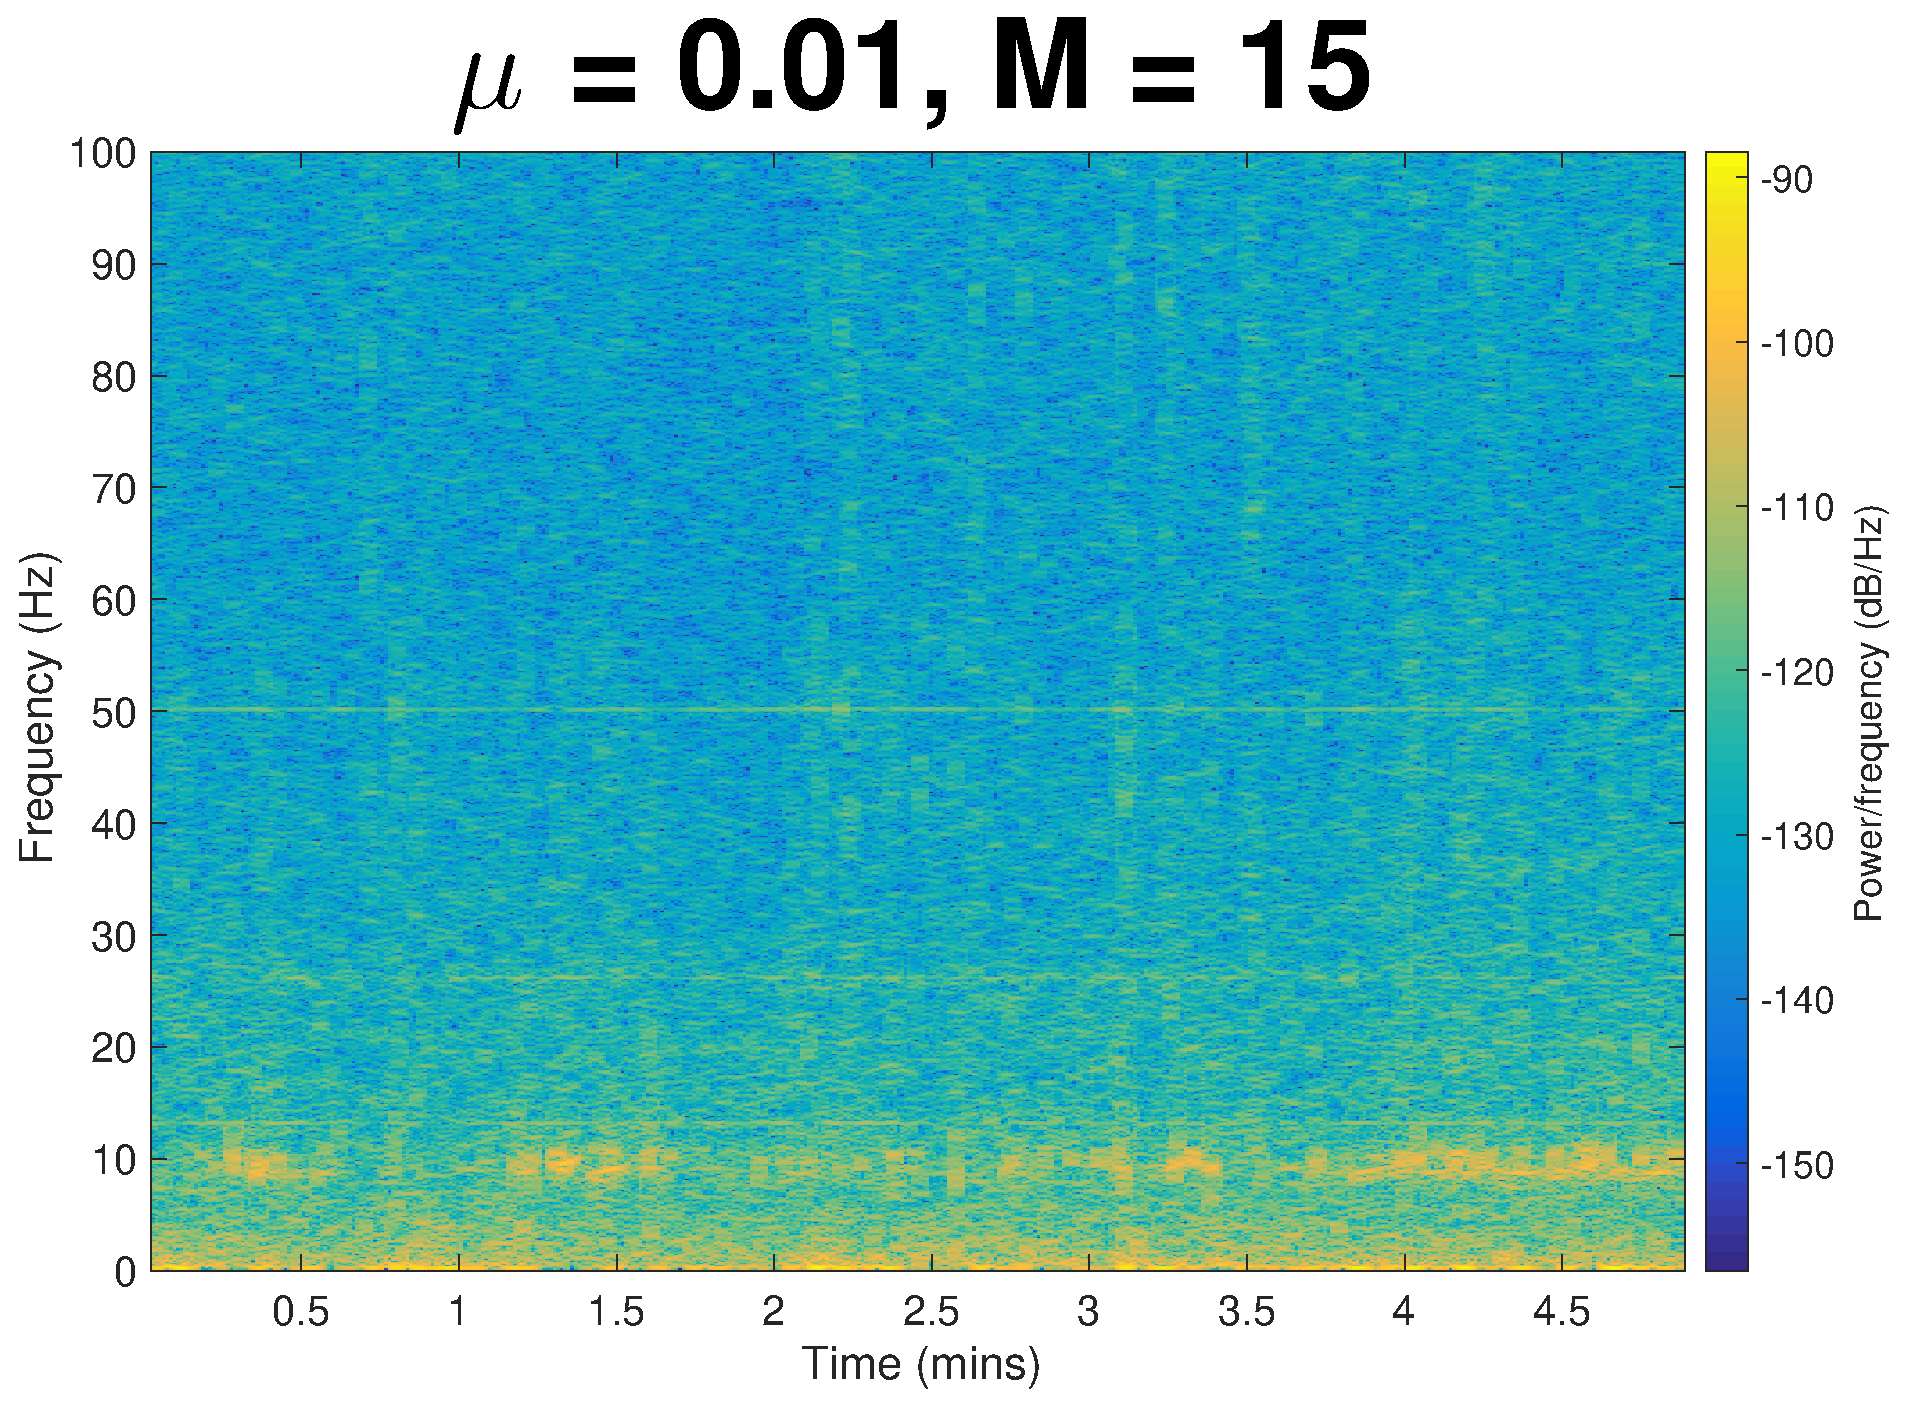
\includegraphics[width=0.24\textwidth]{part3/POz_mu_01_M_15}
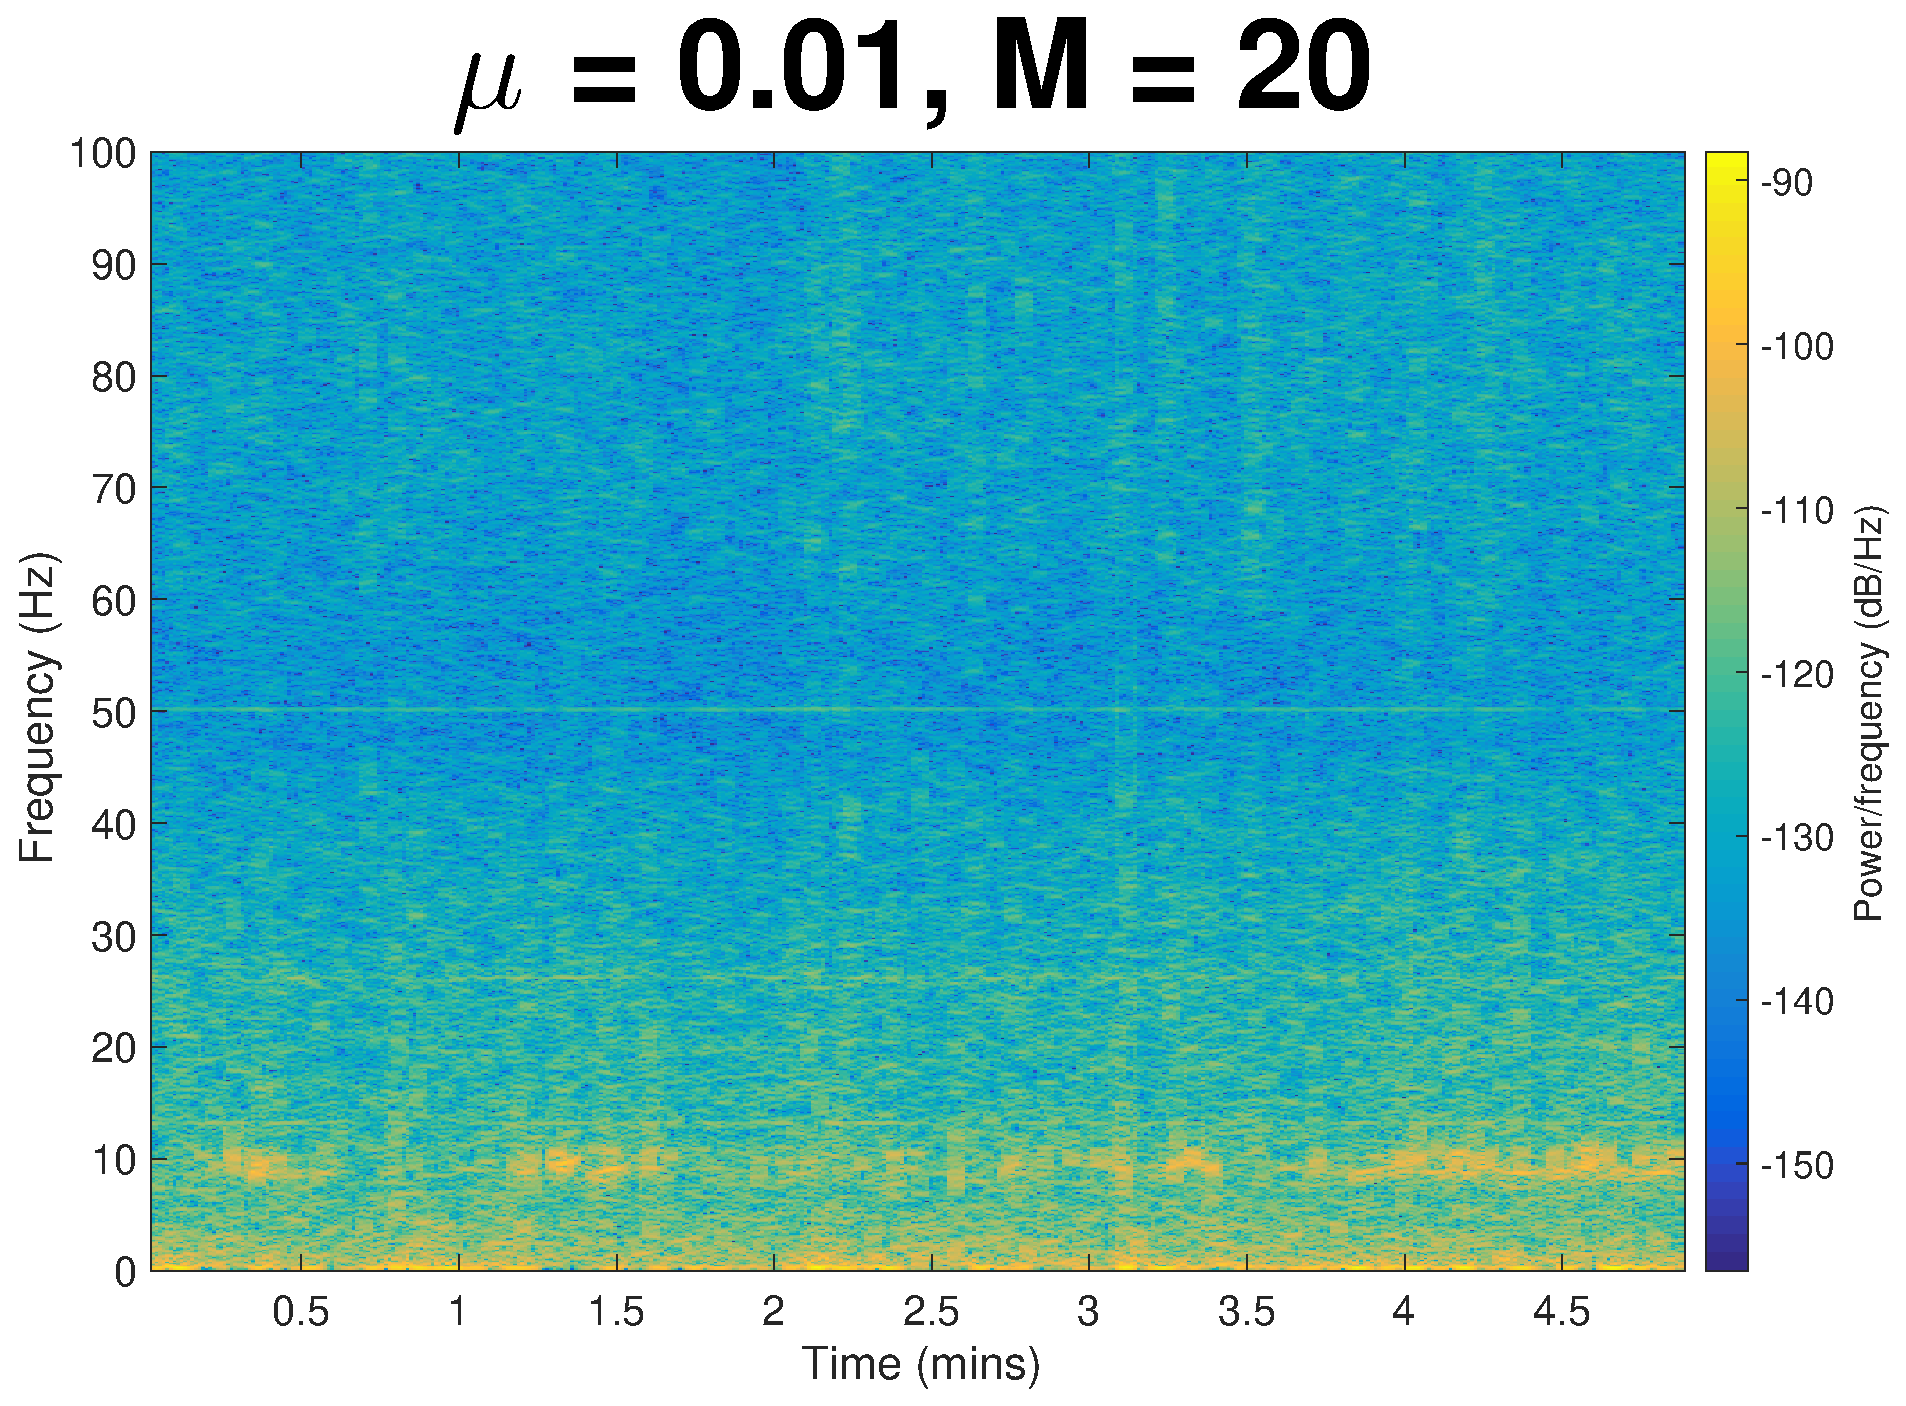
\includegraphics[width=0.24\textwidth]{part3/POz_mu_01_M_20}
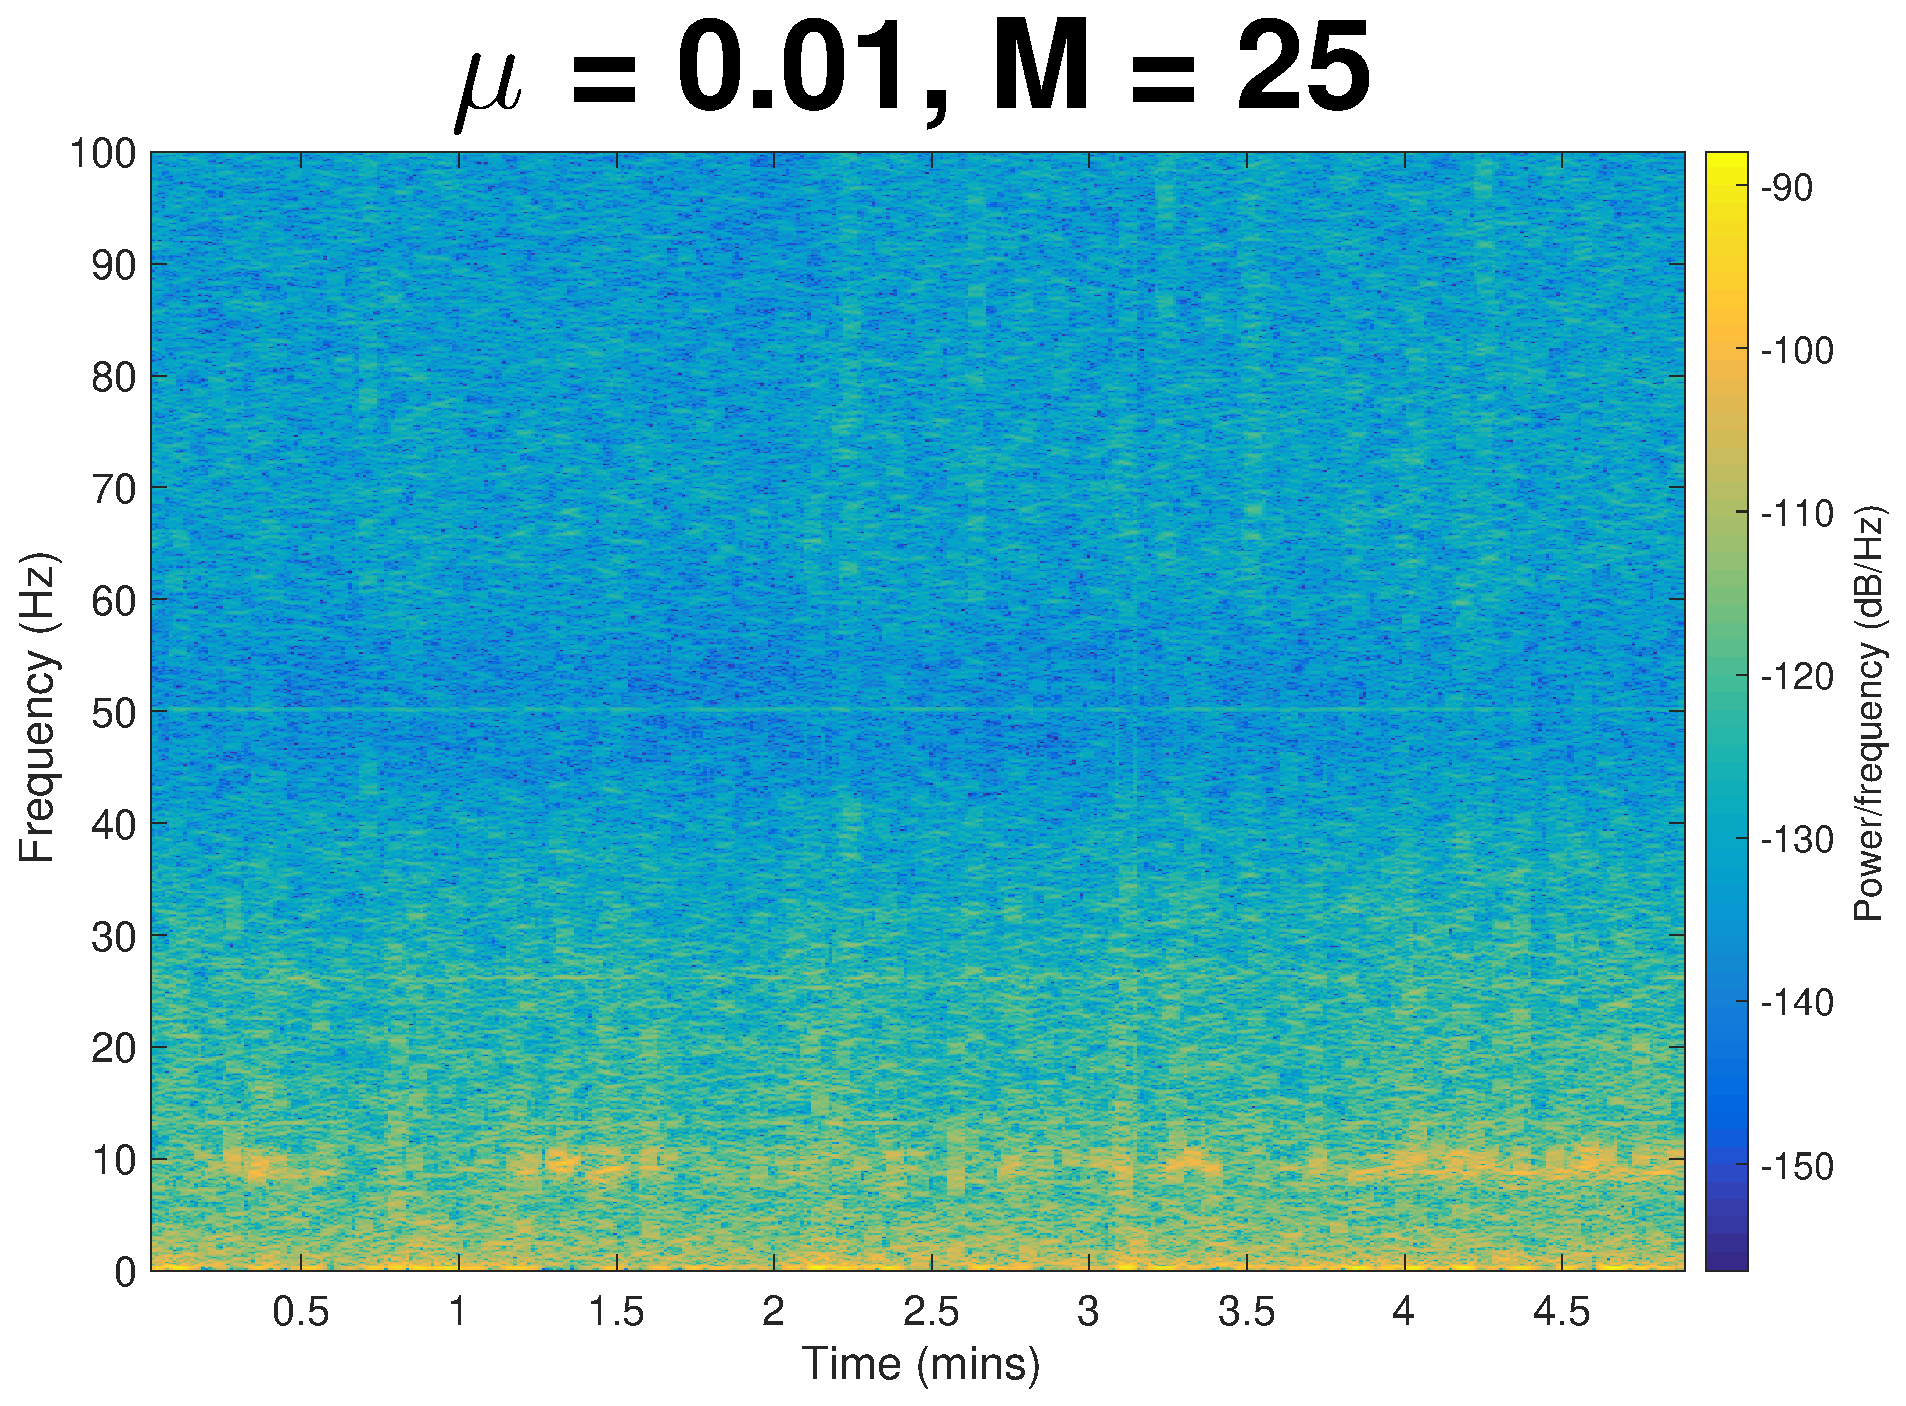
\includegraphics[width=0.24\textwidth]{part3/POz_mu_01_M_25}
\caption{Effect of Increasing Model Order on the Spectrogram of EEG Data}
\end{figure}

\noindent{}To combat the large spread of frequencies over which the filter is acting, we vary $\mu$. The figure below shows the effects of decreasing $\mu$. Decreasing $\mu$ reduces the range of frequencies over which the ANC algorithm acts and leads to better performance. It is clear that the filter is now acting over a much smaller and targeted range of frequencies. 

\begin{figure}[H]
\centering{}
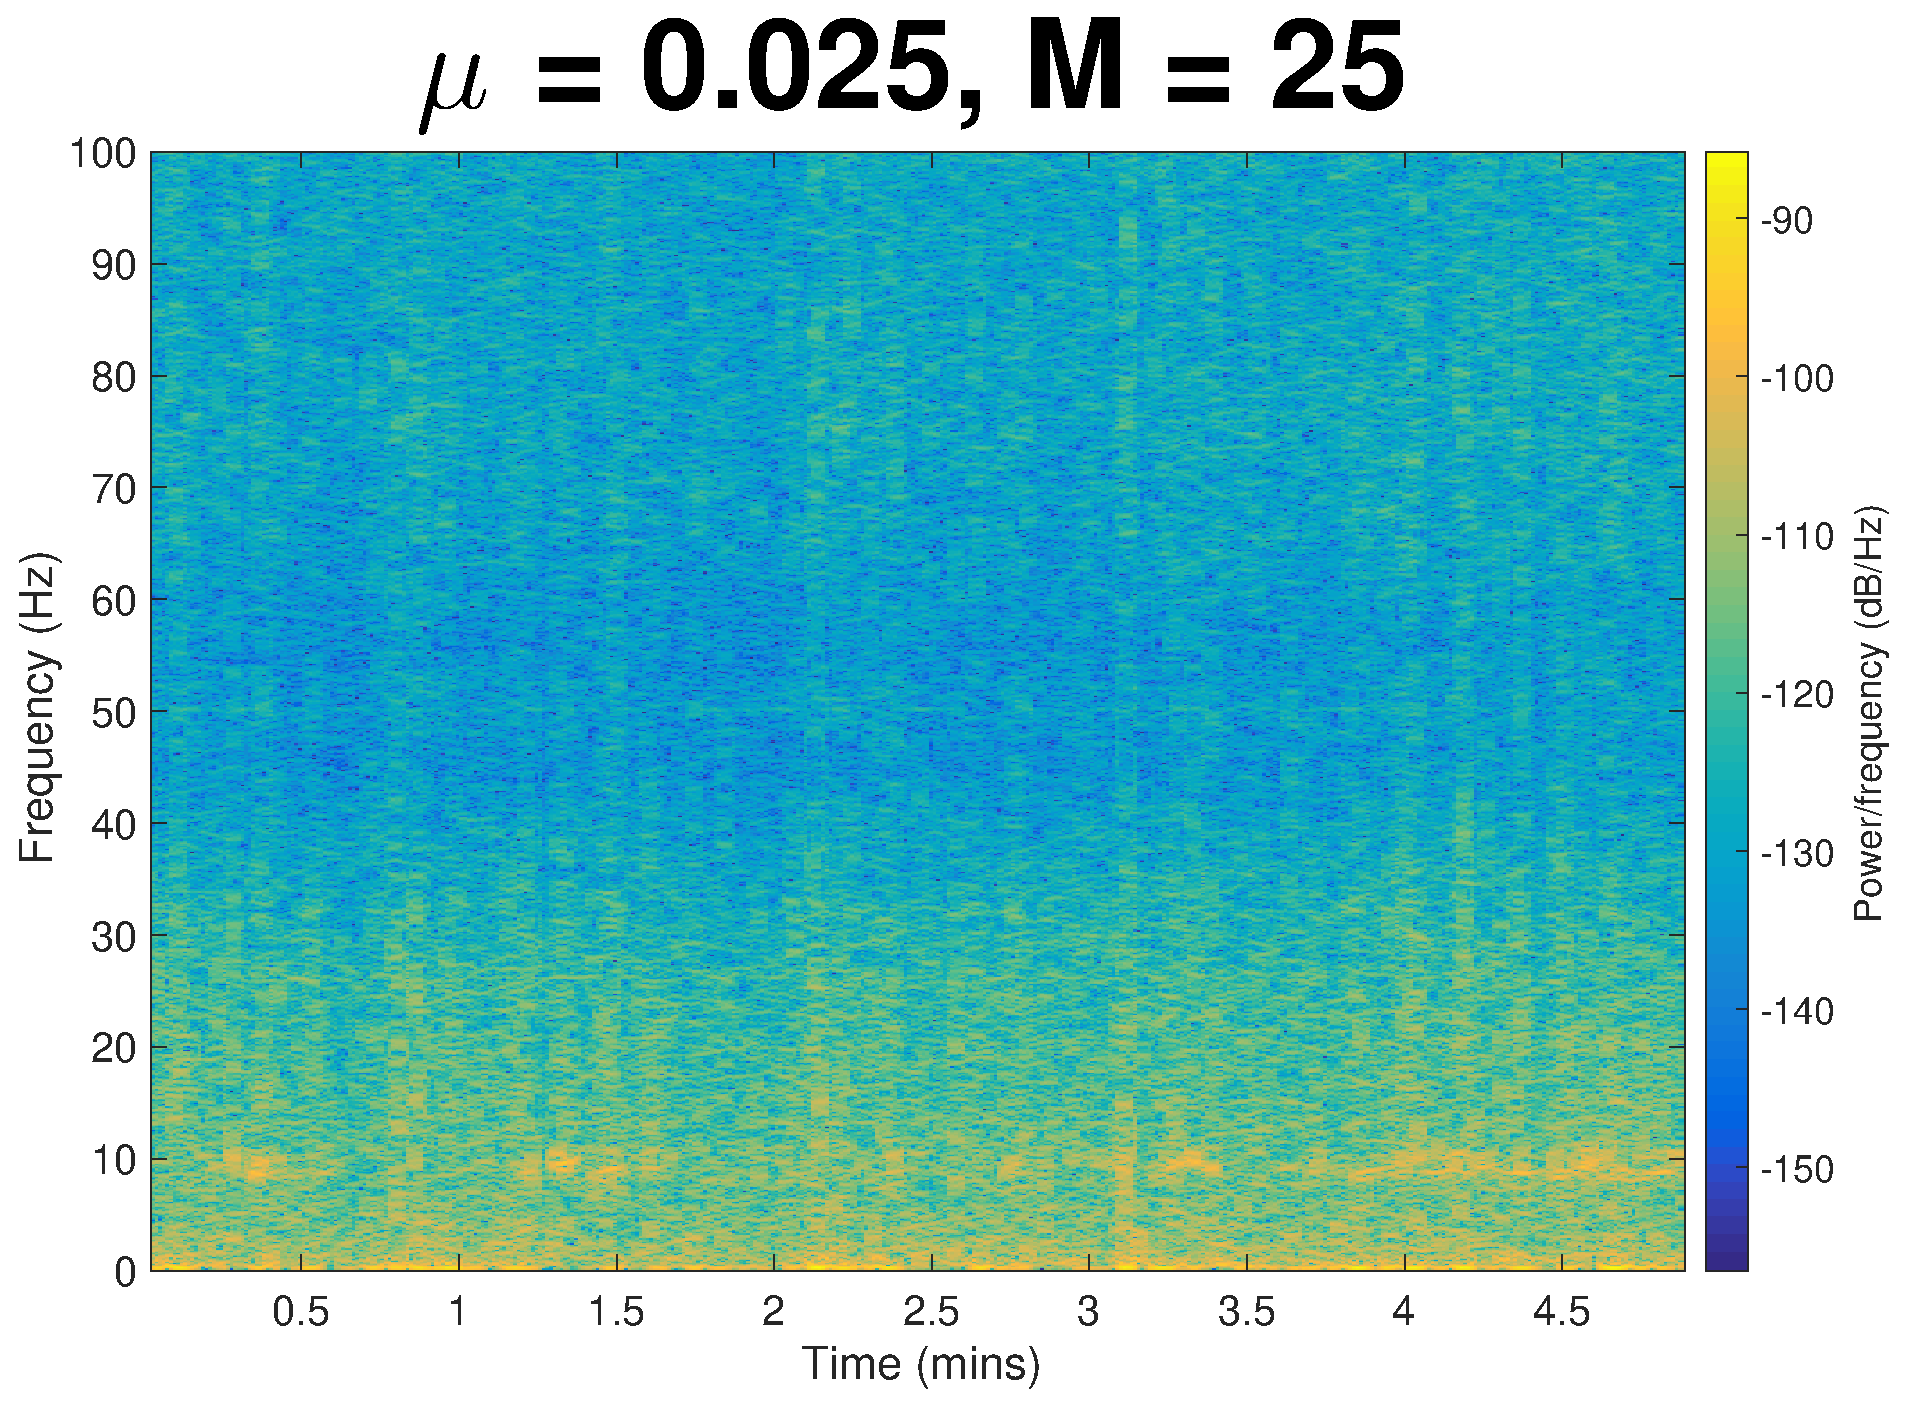
\includegraphics[width=0.24\textwidth]{part3/POz_mu_025_M_25}
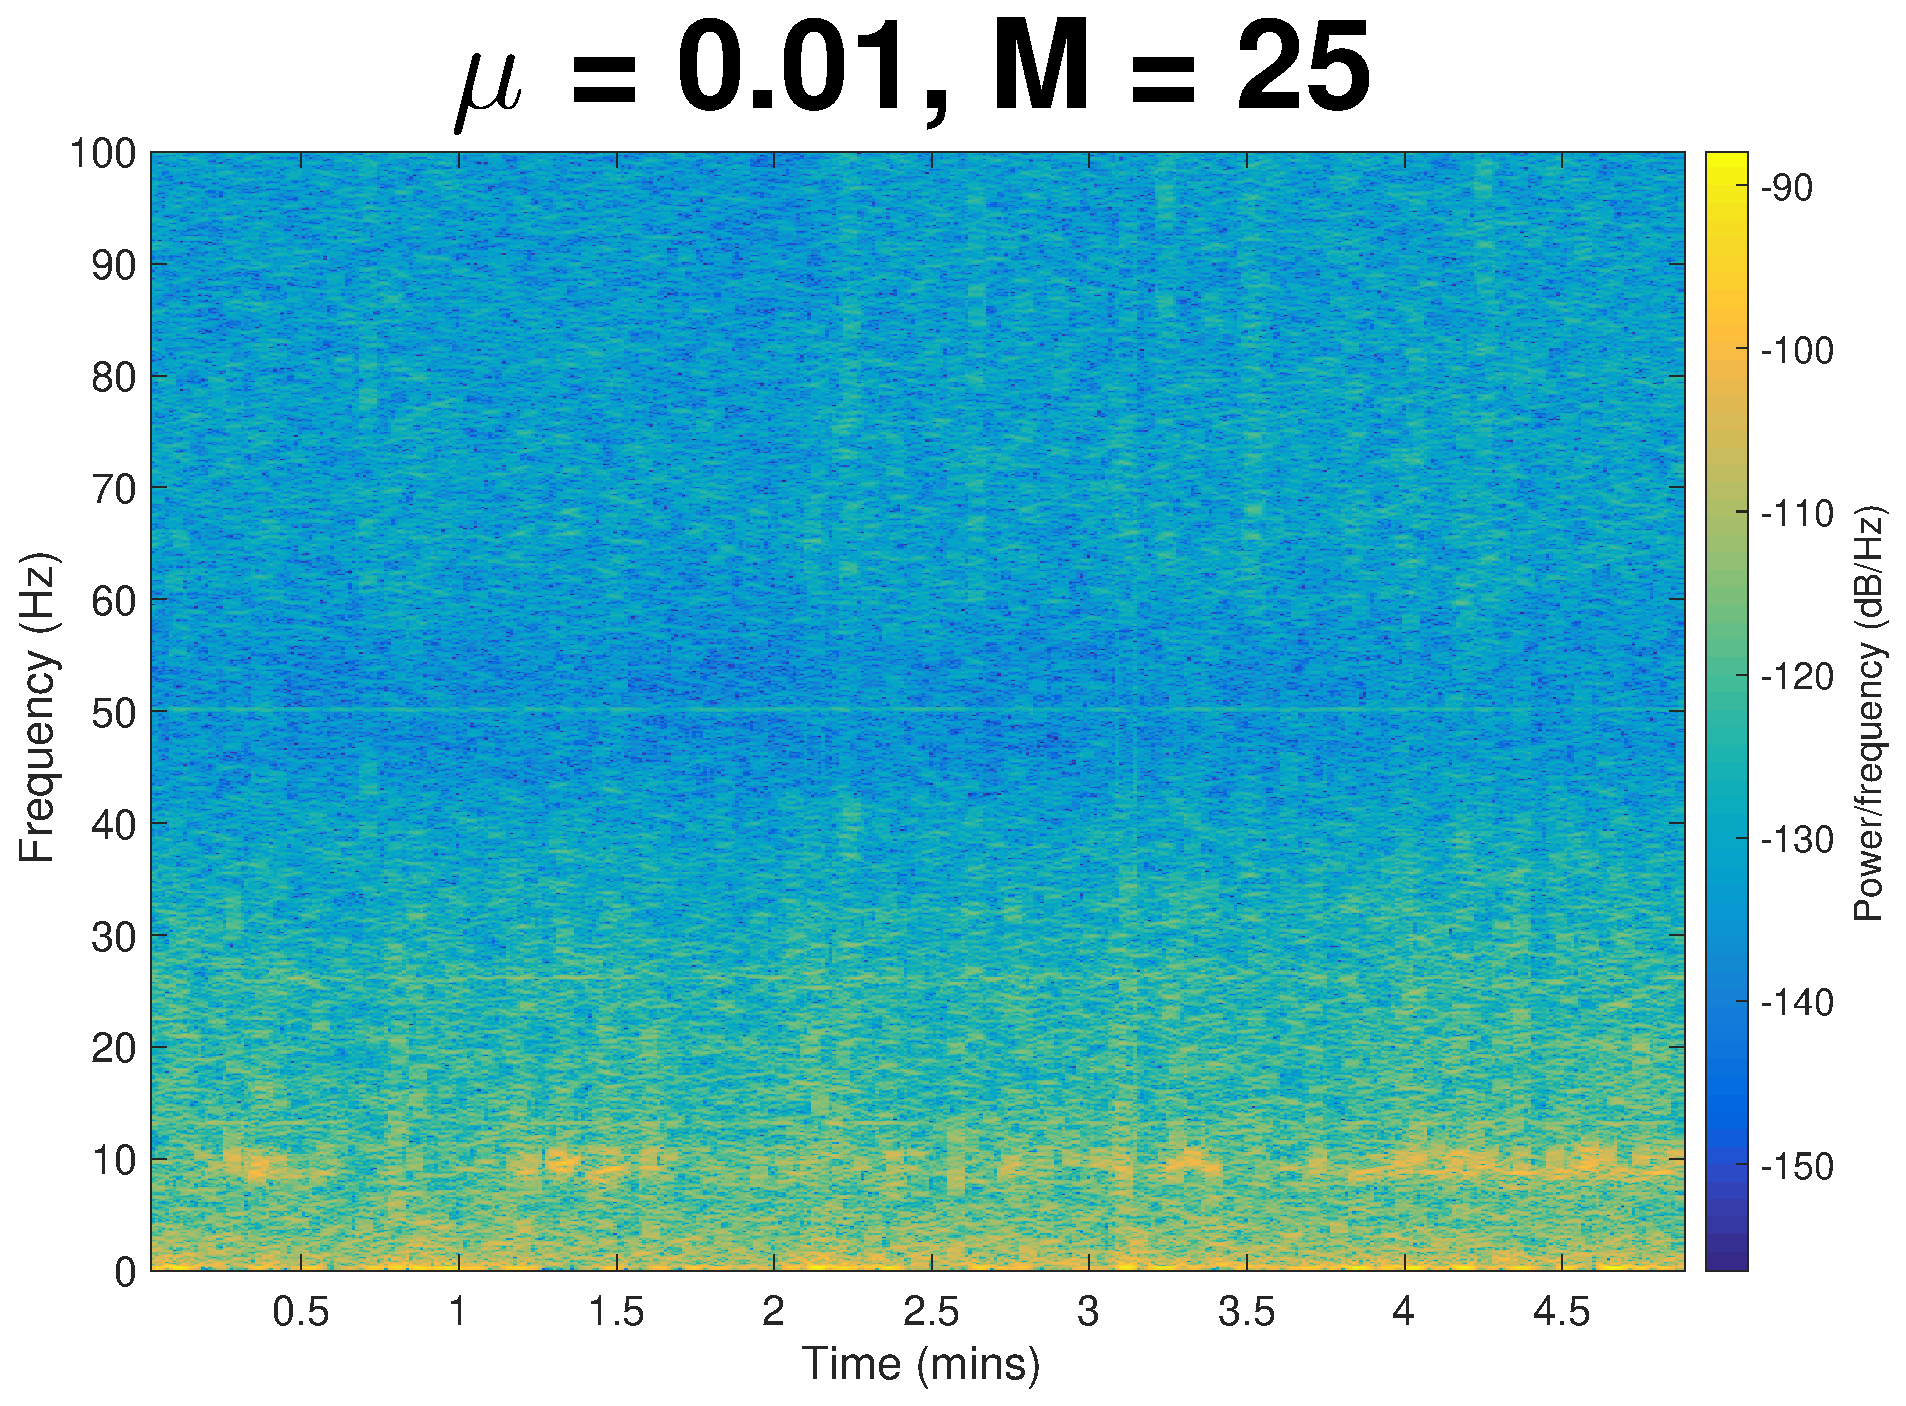
\includegraphics[width=0.24\textwidth]{part3/POz_mu_01_M_25}
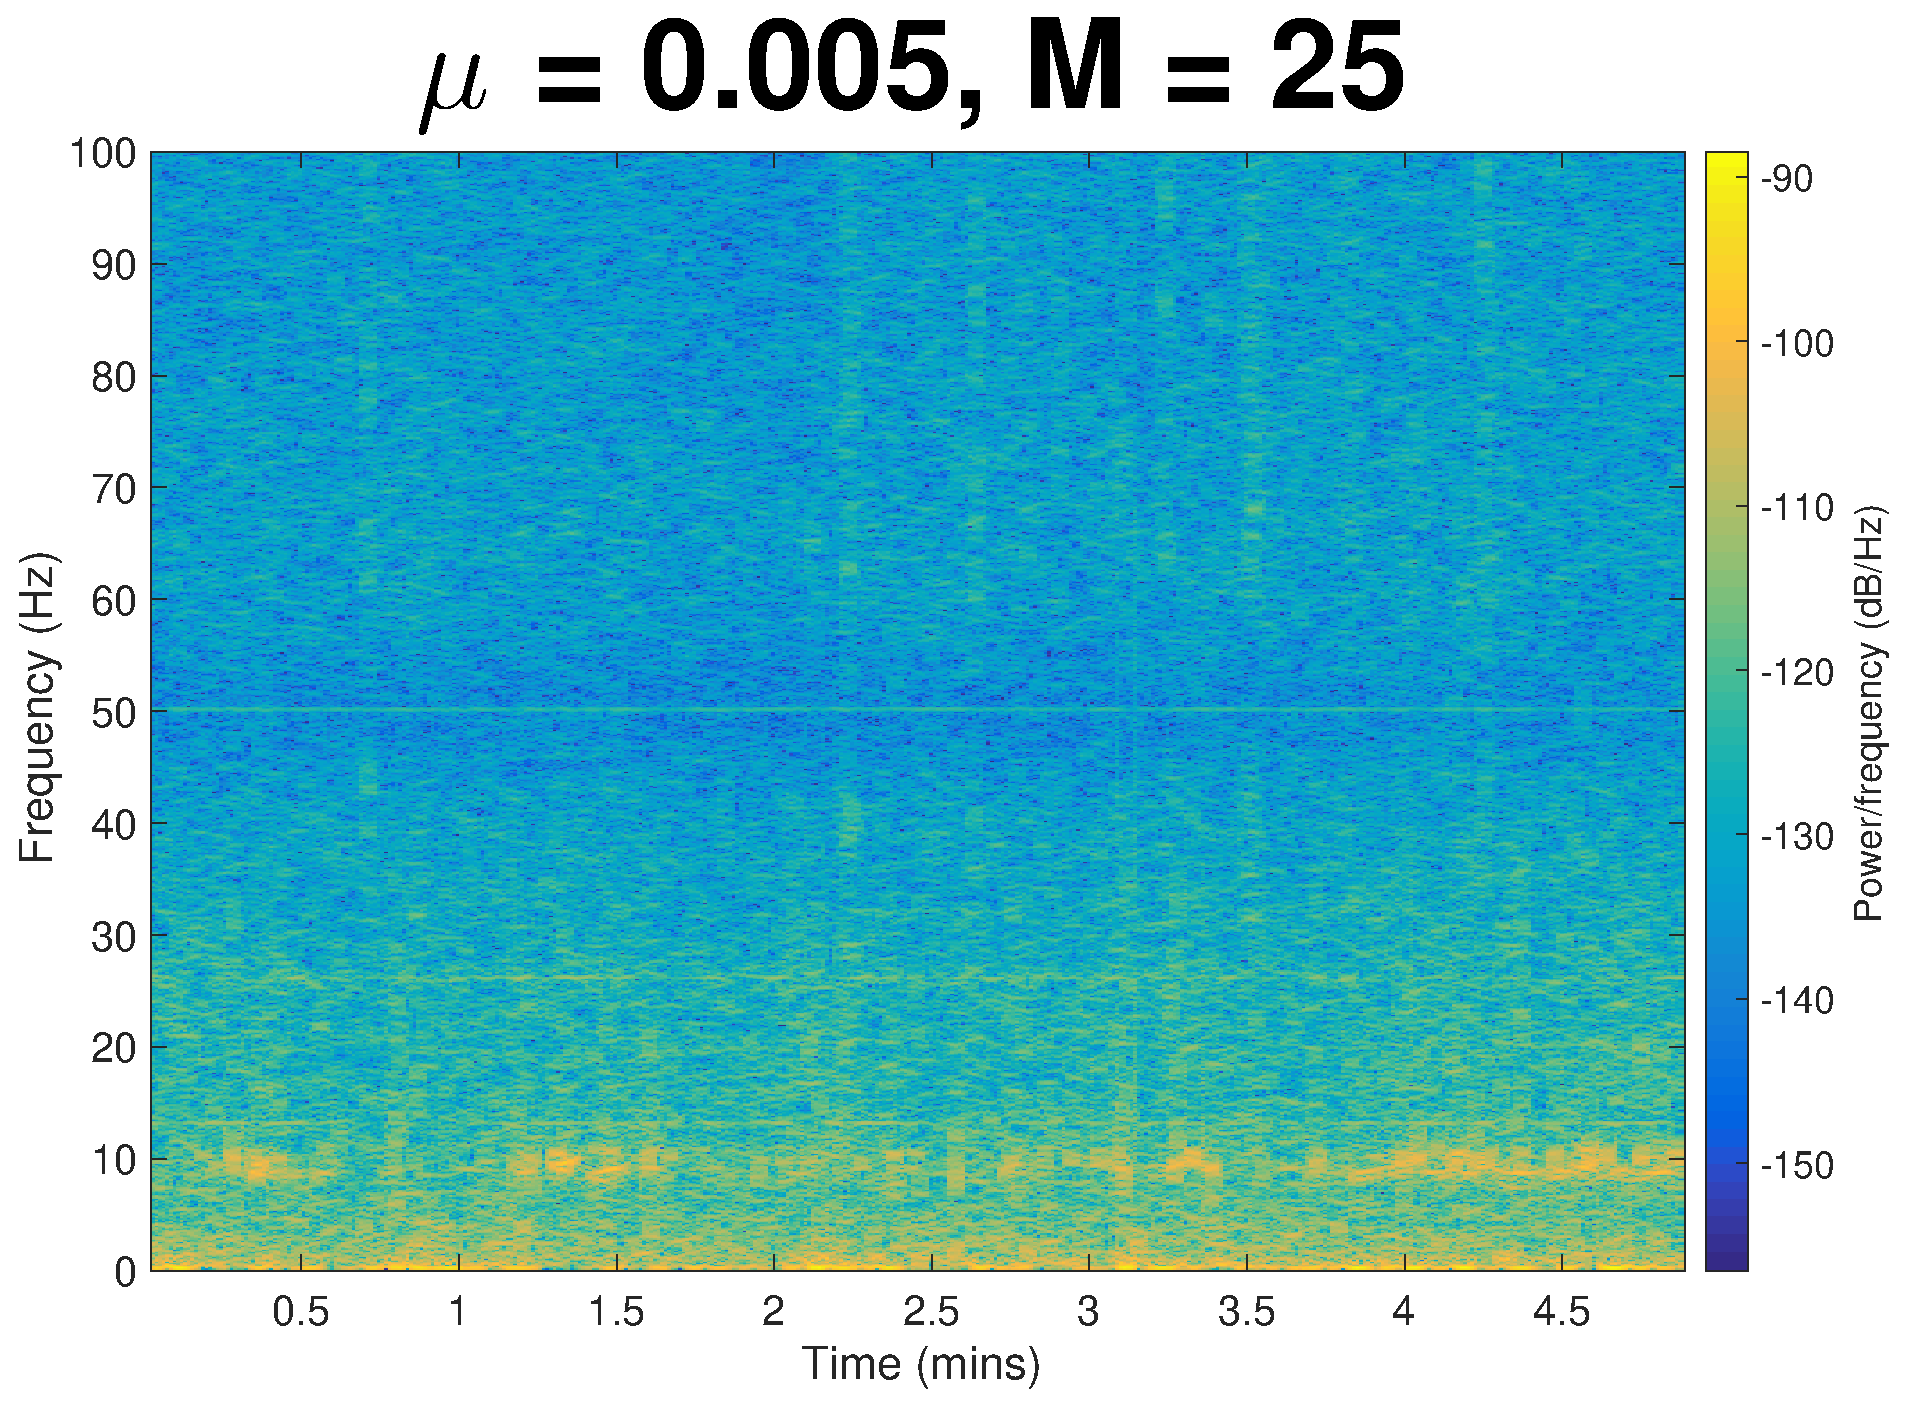
\includegraphics[width=0.24\textwidth]{part3/POz_mu_005_M_25}
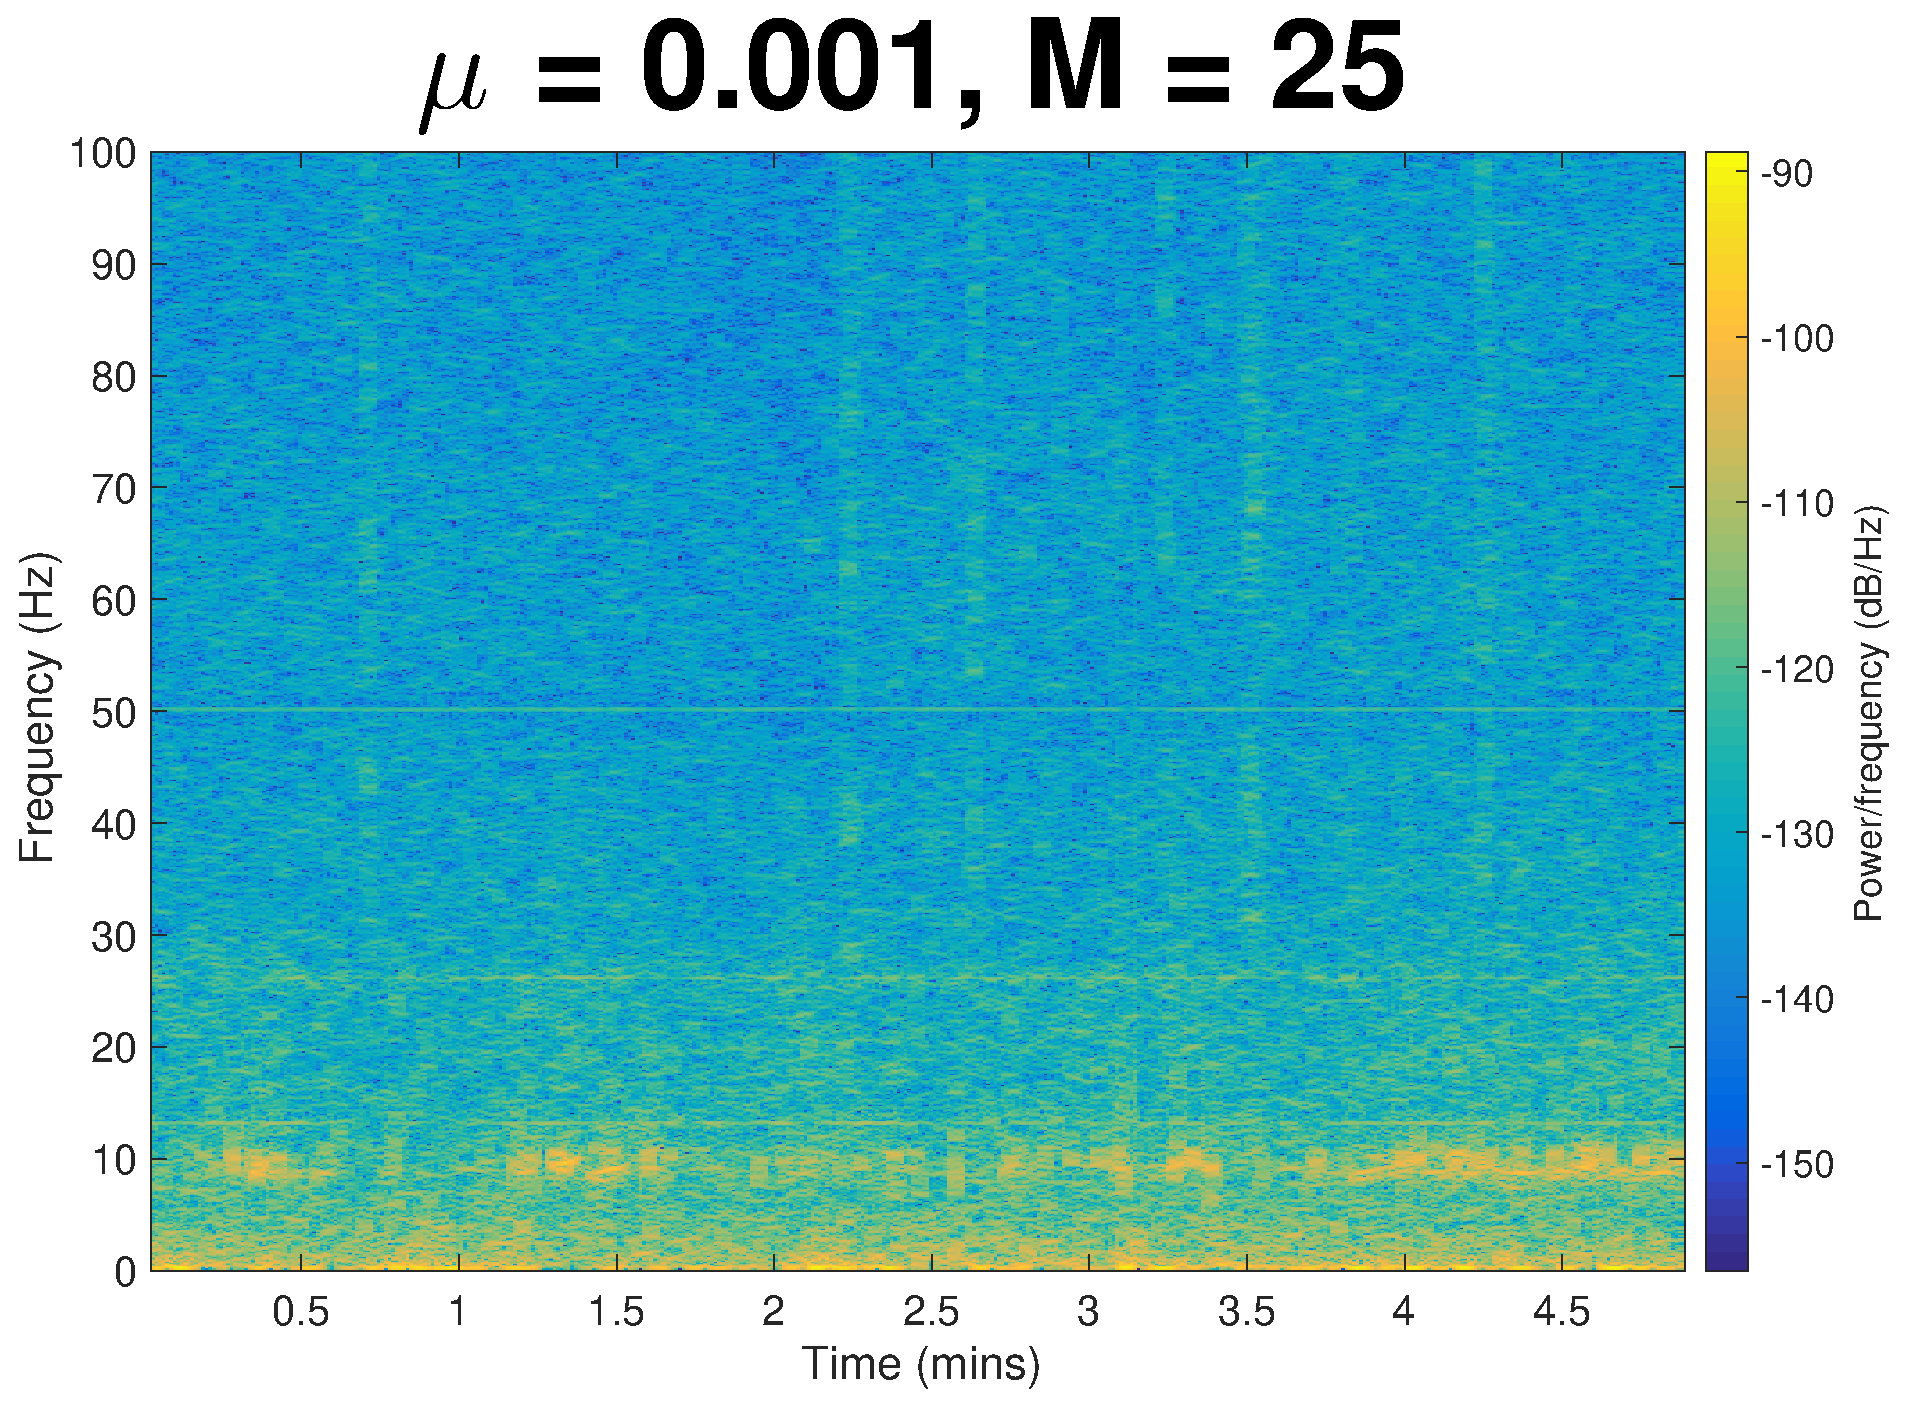
\includegraphics[width=0.24\textwidth]{part3/POz_mu_001_M_25}
\caption{Effect of Varying $\mu$ on the artifacts observed in the Spectrogram of Denoised EEG Data}
\end{figure}


\noindent{}The periodogram and squared error plots corroborate the findings above. For large values of $\mu$ such as 0.025, large errors are incurred at low frequencies. This does not occur with $\mu=0.001$.

\begin{figure}[H]
\centering{}
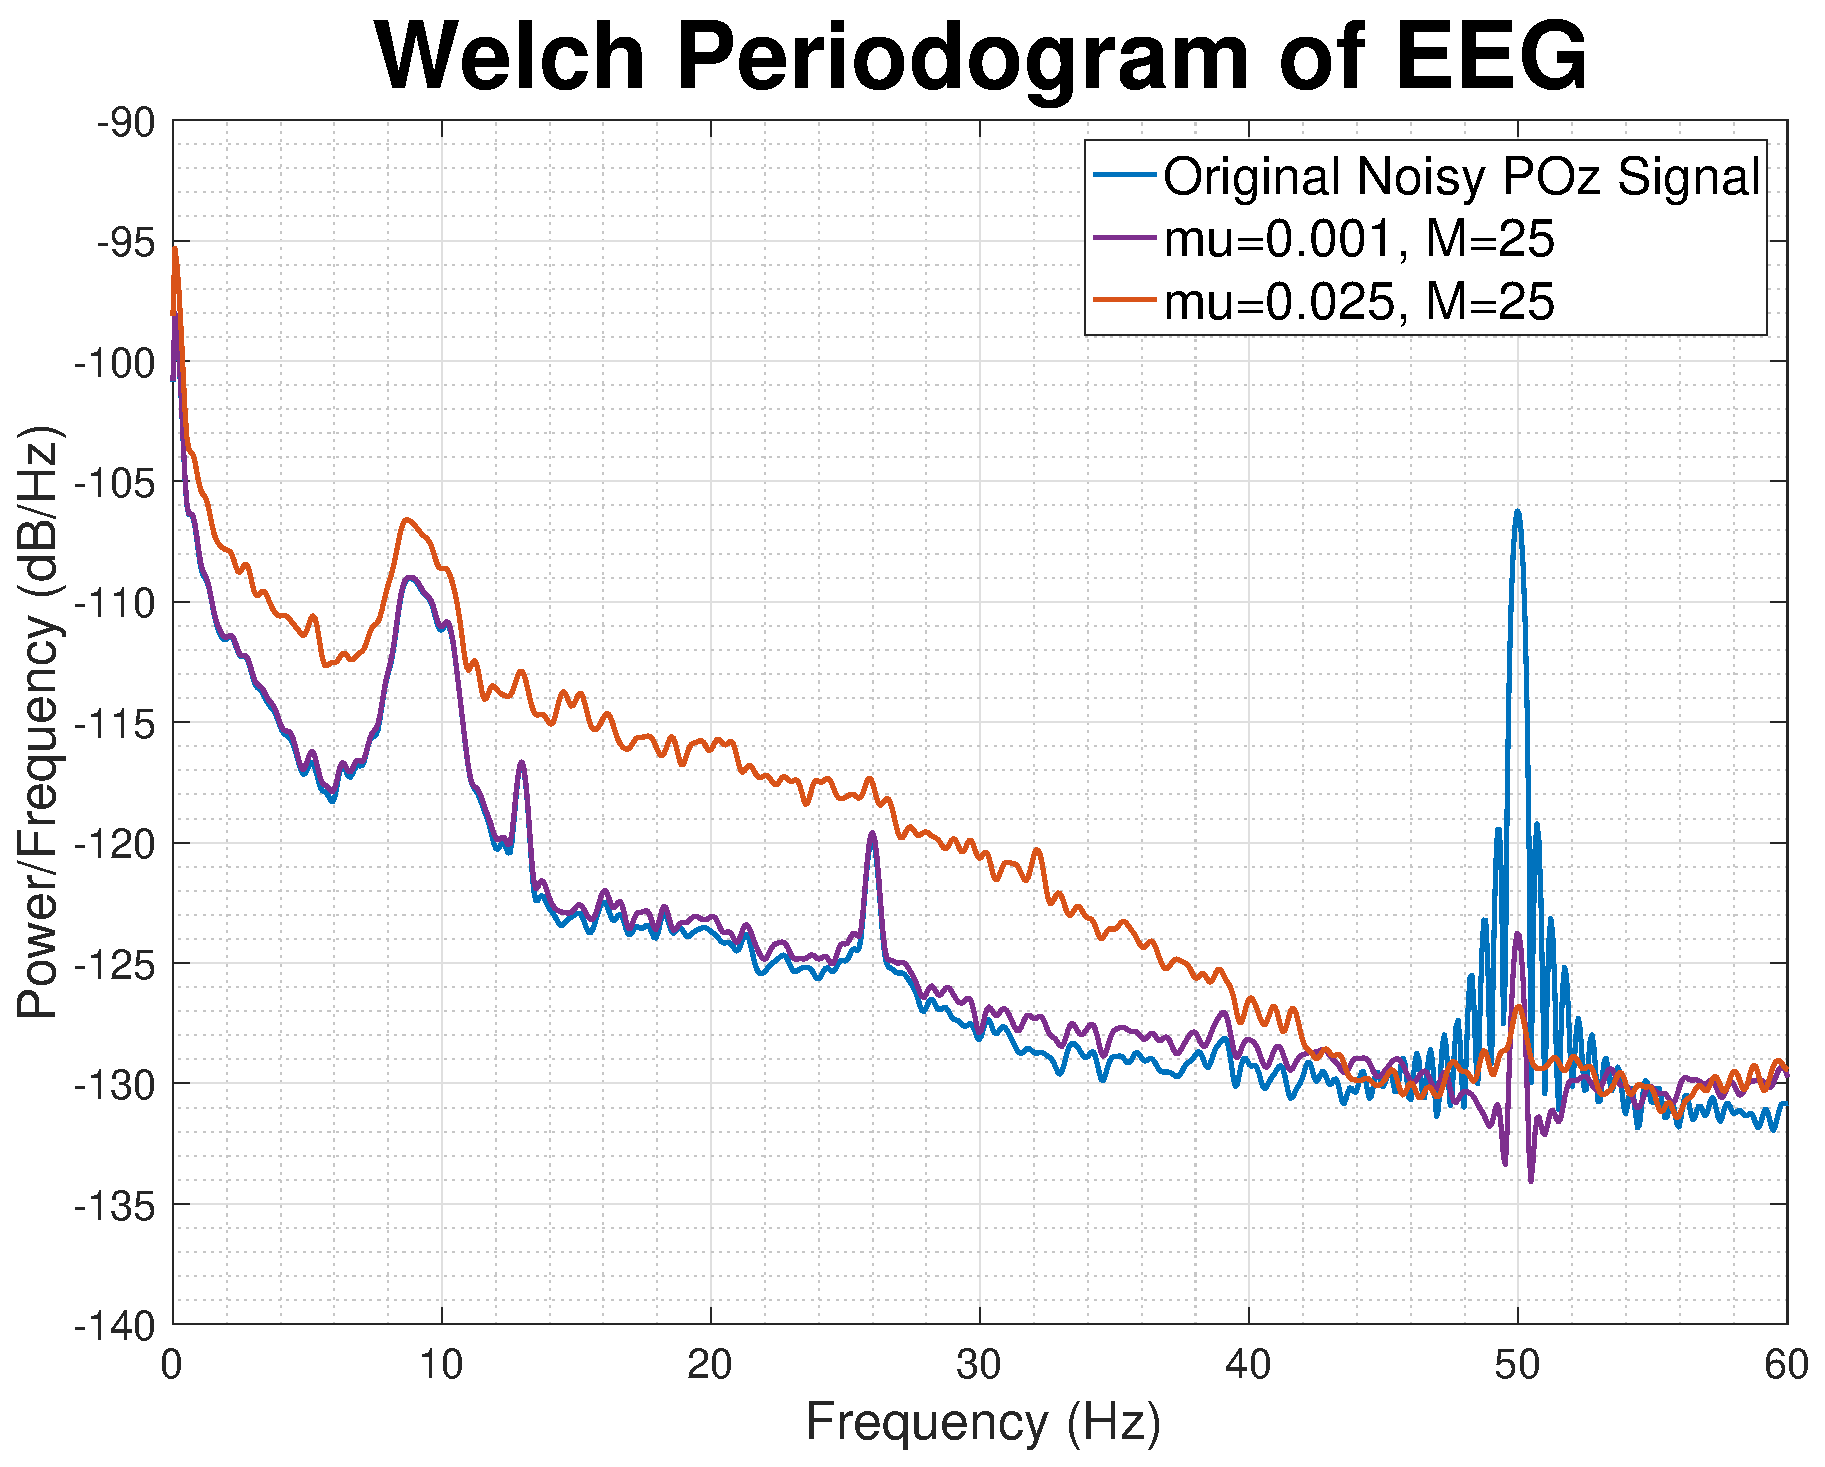
\includegraphics[width=0.32\textwidth]{part3/bartlett_cleaned_Poz}
\includegraphics[width=0.32\textwidth]{part3/squared_error_periodogram}
\includegraphics[width=0.32\textwidth]{part3/squared_error_periodogram_bad}
\caption{Welch Periodogram, averaged over 2 second intervals, and Squared Errors}
\end{figure}
